\begin{abstract}
Wir wollen untersuchen, wie Quanten-Annealing für Reinforcment-Learning genutzt werden kann. Dafür nutzen wir Q-Learning mit einer $\epsilon$-Greedy-Strategie. Die Q-Funktion approximieren wir dabei mit einer Boltzmann-Maschine. Dabei repräsentiert der sichtbare Layer den Zustand und die Aktionen. Die Aktivierung des nicht-sichtbaren Layern können wir mit einem Quanten Annealer berechnen, bzw klassisch simulieren. Als Umgebung für unseren Agenten nutzen wir den ``zugefrorenen See'', ähnlich zu der bekannten Problemstellung von OpenAi mit kleinen Modifizierungen. Wir vergleichen diese Quanten Boltzmann Maschine anschließend mit eine einfachen Q-Tabelle, mit einem einfachen neuronalen Netz von PyTorch und mit einer Beschränkten Boltzmann Maschine.
\end{abstract}

\section{Einleitung }
\label{sec:int}

Reinforment Learning ist ein sehr spannender Bereich innerhalb von maschinellem Lernen, da hier wenig vorarbeit vom Menschen geleistet werden muss. Wir brauchen keine Trainingsdaten manuell zu erstellen, sondern der Algorithmus erstellt seine Trainingsdaten selbst. Gleichzeitig stoßen klassische Rechner hier auch sehr schnell an ihre Grenzen, da die Datensätze sehr groß werden können. Daher ist eine spannende und offene Frage, ob zukünftige Quanten-Computer auch in diesem Bereich irgendwann Vorteile gegenüber klassischen Verfahren haben könnten.

Wir wollen hier eine Methode anschauen, wie wir Quanten-Annealing für eine Deep-Boltzmann-Maschine anwenden können, die Ergebnisse untersuchen und mit klassischen Ansätzen vergleichen.

Als Problem betrachten wir einen Agenten, der eine Frisbee auf einem zugefrorenen See finden muss. Es gibt jedoch Löcher im Eis. Der Agent startet auf einer Startposition und kann sich nun wie auf einem Schachbrett Feld für Feld über den See bewegen. Fällt er dabei in ein Loch, hat er verloren und bekommt 0 Punkte. Findet er den richtigen Weg zur Frisbee, hat er gewonnen und bekommt 1 Punkt. Wir versuchen also den kürzesten Weg vom der Startposition zur Frisbee zu finden, ohne dabei in ein Loch zu fallen.

Ein bekanntes Problem dabei ist, dass wir einen guten Ausgleich zwischen Erkunden und bekannte Informationen verwenden finden wollen. Allgemeiner betrachtet, weiß der Agent nicht, wie viele Frisbees es gibt und wie viele Punkte er in dem Spiel bekommen kann. Daher will er möglichst viele Felder und Wege erkunden, bevor er sich einen konkreten Weg aussucht, den er bei jedem Spiel geht. Gleichzeitig will der Agent aber auch schnell die richtige Strategie finden, was konkret heißt, dass der Computer weniger Rechenzeit verbraucht, bis er den schnellsten Weg gefunden hat. Dieses Dilema lösen wir mit der $\epsilon$-Greedy-Strategie.

Um die beste Aktion von einem gegebenen Feld zu finden, müssen wir die Aktionen bewerten. Die einfachste Möglichkeit dafür ist eine sogenannte Q-Tabelle, die für jedes Feld jedem Zug einen Wert zuordnet.

Eine mächtigere aber auch komplexere Möglichkeit ist, die Aktionen mit einer Q-Funktion zu bewerten, die durch ein neuronales Netz realisiert wird. Dafür können wir beliebige neuronale Netze auswählen und mit bekannten Optimierungsmethoden trainieren. Eine Boltzmann-Maschine ist dabei besonders interessant, da die Struktur einer Deep-Boltzmann-Maschine sehr ähnlich zu der Struktur von einem Ising Model in einem Quanten-Annealer ist. So können wir die Aktivierung des nicht-sichtbaren Layers auf dem DWave oder alternativ mit simuliertem Quaten-Annealing brechnen.

\section{Problemstellung}
\label{sec:prob}

\subsection{Umgebung}
\label{subsec:umg}

Als erstes wollen wir genau definieren, wie unsere Umgebung/das Spielfeld aussieht und welche Regeln es gibt. Wir haben also ein Spielfeld ähnlich wie ein Schachbrett mit verschiedenen Feldern. Der Agent wird am Anfang auf ein Startfeld gesetzt, was sich in der Regel in einer der Ecken befindet. Von diesem Startfeld kann er nun in eine der vier Richtungen (links, unten, rechts, oben) einen Zug machen und sich ein Feld bewegen. Falls er sich mit diesem Zug vom Spielfeld bewegen würde, passiert nichts und er bleibt auf seinem Feld. Ist das Feld auf das er zieht ein Loch, wird das Spiel beendet und der Agent hat verloren. Das wird dadurch symbolisiert, dass er 0 Punkte bekommt. Ist das Feld auf das er zieht das Ziel, dann wird das Spiel auch beendet und der Agent bekommt einen Punkt als Belohnung. Falls das Feld leer ist, bewegt sich der Agent auf das Feld und der Agent kann einen weiteren Zug machen.

Unten sehen wir Beispielhaft zwei Spielfelder. In den Grafiken unten steht S für Start, Z für Ziel und L für Loch:

\begin{figure}[H]
\centering
\includegraphics[width=\textwidth]{Figures/advanced1.png}
\caption{4x4 Feld}
\label{advanced1}
\end{figure}

\begin{figure}[H]
\centering
\includegraphics[width=\textwidth]{Figures/advanced2.png}
\caption{3x5 Fekd}
\label{advanced2}
\end{figure}

\subsection{Varianten der Umgebung}
\label{subsec:vars}

Unsere Variante ist eine etwas abgewandelte Version von der ``Frozen-Lake'' Umgebung die aus der Library Gym von OpenAi stammt. In der Originalversion gibt es allerdings Unterschiede: Zum einen wird der Agent zurück aufs Startfeld gesetzt, wenn er das Spielfeld verlässt. Und zum anderen ist das Feld in den Standardeinstellungen ``rutschig''. Das heißt wählt der Agent für den nächsten Zug z.B. rechts aus, gibt es eine bestimmte Wahrscheinlichkeit, dass der Agent auch wirklich nach rechts geht. Ansonsten macht er einen zufälligen Zug. Beide Bedingungen machen das Spiel schwerer.

In \citep{crawford2019reinforcement}, gibt es dagegen noch eine fünfte Aktion ``auf der Stelle bleiben''. Außerdem endet das Spiel nach einer festen Anzahl von Zügen und der Agent hat z.B. die Möglichkeit eine Belohnung öfter zu bekommen, indem er auf dem Zielfeld mehrere Züge bleibt. Die Löcher werden dann durch ``Bestrafungen'' ersetzt und der Agent kann über diese Felder gehen. Dies ist also eine einfachere Version, da der Agent leichter zum Ziel kommt und die Belohnungen öfter einsammelt und damit öfter lernen kann. Außerdem werden zusätzlich Wände eingeführt, also im Prinzip Felder auf die der Agent nicht gehen kann. Die Grenzen des Spielfeldes sind auch Wände, dadurch reduzieren sich an den Randfeldern auch die Anzahl der möglichen Züge.

Wir haben uns für unsere Variante entschieden, da wir so mit durch den Ähnlichkeit mit OpenAi bessere Vergleichbarkeit zu bekannten Methoden haben. Gleichzeitig haben wir die Variante vom ``Frozen-Lake'' etwas vereinfacht, da eine komplexe Boltzmann-Maschine sich beim lernen etwas schwerer tut, als eine einfache Q-Tabelle wie sie bei OpenAI verwendet wird. Dafür kann eine Boltzmann-Maschine komplexere Zusammenhänge zwischen Zuständen und Aktionen erkennen. Dies hilft uns für diese Umgebung nicht, man sollte dies jedoch im Hinterkopf behalten, wenn man die Resultate vergleicht.

\subsection{Darstellung der Umgebung}
\label{subsec:darstellung}

In Folgenden werden wir die Position auf dem Spielfeld als Zustand und die Züge als Aktionen bezeichnen. Wir haben damit für jedes Feld einen möglichen Zustand. Für den menschlichen Verstand ist es vorteilhaft sich das Feld als Matrix vorzustellen mit Reihen und Spalten. Dann werden alle Einträge der Matrix auf 0 gesetzt und das Feld auf dem wir stehen, wird auf 1 gesetzt. Um die Zustände aber besser in einem Algorithmus verwenden zu können, verwandelt wir ihn in einen einzelnen Vektor, wo wiederum jeder Eintrag für ein Feld steht.

In gleichem Sinne haben wir einen Vektor für die Aktionen, wobei der erste Eintrag für links, der zweite für unten, der dritte für rechts und der vierte für oben steht.

Die Umgebung wird auch durch eine Matrix dargestellt, wobei eine 1 für das Ziel steht und eine -1 für ein Loch. Die restlichen Einträge sind 0.

\subsection{Der Agent}
\label{subsec:agent}

Der Agent ist unsere Intelligenz, die sich über das Spielfeld bewegt. Ein Agent hat eine Methode wie er lernt, die beim Erstellen des Agenten ausgewählt wird. Mit dieser Methode kann er einen Zug auswählen und er kann aus einem gemachten Zug lernen. Er kann also abwechselnd Züge machen und daraus lernen, bis er hoffentlich nach genügend Spielen gelernt hat, welche Aktionen in welchem Zustand am besten ist. Dies nennt man die Police des Agenten. Am Anfang ist sie bei den meisten Methoden zufällig und wird dann durch das Lernen stück für stück verbessert.

Betrachten wir als Beispiel eine bestmögliche Police für unser 4x4 Beispiel von oben.

\begin{figure}[hbt!]
\centering
\includegraphics[width=\textwidth]{Figures/advanced1police.png}
\caption{Beispiel einer optimalen Police}
\label{police}
\end{figure}

Um diesen Lernvorgang sinnvoll zu gestalten nutzen wir die $\epsilon$-Greedy-Strategie. Wir spielen insgesamt 10000 Spiele wobei $\epsilon$ zu beginn auf 1 gesetzt wird. Jetzt wird eine Aktion zufällig gewählt. Nach jedem Spiel wird $\epsilon$ etwas gesenkt, um dann mit einer Wahrscheinlichkeit von $\epsilon$ eine zufällige Aktion zu wählen und sonst den besten Zug, den der Agent anhand seine Police auswählt. Nach 90\% der Spiele ist $\epsilon$ bei 0.01 angekommen, dass heißt wir wählen mit 99\% Wahrscheinlichkeit einen Zug nach der Police. So können wir bei den letzten 1000 Spielen beobachten, ob unser Agent die richtige Police gelernt hat.

Die $\epsilon$-Greedy-Strategie hat den Vorteil, wirklich einen Roboter zu simulieren, der auf unbekannten Gelände unterwegs ist und aus seinen Aktionen lernt. Allerdings stößt sie schnell an ihre Grenzen, nämlich genau dann, wenn am Anfang vom Start aus durch zufällige Aktionen das Ziel fast nie gefunden wird. Tatsächlich passiert dies in unserer Version mit den Löchern die das Spiel beenden sehr schnell. Daher haben wir zwei Alternativen: Zum einen können wir verschiedene Startpositionen wählen, die erst nah am Ziel sind und sich dann weiter weg bewegen. Zum anderen können wir geordnet von jedem Feld jeden Zug machen und jeweils daraus lernen. Letzteres funktioniert natürlich viel besser, entspricht aber dann nicht mehr einem echten Spiel. Dafür können wir hier schauen, wie robust die Verfahren sind, wenn die Zustandsräume sehr groß werden.

\subsection{Markov-Entscheidungsprozess}
\label{subsec:mdp}

Ein Markov-Entscheidungsprozess ist ein zeitlich diskreter, stochastischer Steuerungsprozess. Hier soll ein Agent Entscheidungen treffen, wonach sich der Zustand mit einer bestimmten Wahrscheinlichkeit ändert.

Konkret ist ein Markov-Entscheidungsprozess ein Tupel $(S, A, \mathbb{P}, r, \gamma, \pi)$, wobei:

\begin{itemize}
 \item S eine endliche Menge von Zuständen ist
 \item A eine endliche Menge von Aktionen ist
 \item $\mathbb{P}(s^{\prime} \in S | s \in S, a \in A)$ gibt für jede Kombination aus einem Zustand s und eine Aktion a, die Wahrscheinlich an, mit der wir in Zustand $s^{\prime}$ landen
 \item $r(s,a)$ ist eine Funktion in die rellen Zahlen, welche uns für einen Zustand s und eine Aktion a die Belohung ausgibt
 \item $\gamma \in [0,1)$ ist ein Diskontierungsfaktor für Belohungen in folgenden Zeitschritten
 \item $\pi$ ist die Police, die uns für jeden Zustand angibt, welchen Zug wir als nächstes ausführen
\end{itemize}

Unsere Umgebung die wir weiter oben definiert haben führt uns also zu einem Markov-Entscheidungsprozess.  In unseren Beispielen verwenden wir größtenteils eine Wahrscheinlichkeit von 100\% in dem naheliegenden State $s^{\prime}$ zu landen ($\mathbb{P}(s^{\prime} \in S | s \in S, a \in A) = 1$)  und 0\% sonst ($\mathbb{P}(s^{\prime} \in S | s \in S, a \in A) = 0$).

$r(s,a)$ ist in unserem Beispiel immer 0, es sei den wir landen auf dem Zielfeld, dann gilt $r(s,a) = 1$.

$\gamma$ können wir selbst wählen und wir werden hier später verschiedene Werte testen. $\pi$ wollen wir optimieren, also ein optimales $\pi^{*}$ finden.

\subsection{Value-Funktion}
\label{subsec:V}

Die Value-Funktion gibt für einen Zustand s und eine Police $\pi$ die zu erwartende Belohung an. Also die Belohnung, die vorraussichtlich in diesem und allen weiteren Zeitschritten gesammelt werden kann. Hier benötigen wir den Diskontierungsfaktor $\gamma$, damit der erwartete Gewinn auf jeden Fall endlich bleibt \citep{DBLP:journals/jmlr/SallansH04}

\begin{align}
	V(\pi, s) = \mathbb{E}[\sum\limits_{i=0}^{\infty} \gamma^{i} r(\Pi_{i}^{s},\pi(\Pi_{i}^{s})]
\end{align}

und damit können wir die optimale Police ausdrücken mit:

\begin{align}
	\pi^{*}(s) = argmax_{\pi} V(\pi,s)
\end{align}

Hier gilt es jedoch zu berücksichtigen, dass in unserem Beispiel, das Spiel endet, wenn wir in ein Loch fallen oder das Ziel erreichen. Wir müssen also die Value-Funktion dementsprechend anpassen. Die Summe geht dann nicht bis $\infty$, sondern nur bis zu dem Zug, in dem das Spiel endet.

\subsection{Value-Iteration und Q-Funktion}
\label{subsec:VQ}

Die Value-Funktion können wir mit der Value-Iteration von Bellmann weiter aufteilen \citep{Bellman767}:
\begin{align*}
V(\pi, s) 	&= \mathbb{E}[ \sum\limits_{i=0}^{\infty} \gamma^{i} r(\Pi_{i}^{s},\pi( \Pi_{i}^{s} )] \\
			&= \mathbb{E}[r(s,\pi(s)] + \gamma \mathbb{E}[\sum\limits_{i=1}^{\infty} \gamma^{i} r(\Pi_{i}^{s},\pi(\Pi_{i}^{s})] \\
			&= \mathbb{E}[r(s,\pi(s)] + \gamma \mathbb{E}[\sum\limits_{s^{\prime}} \mathbb{P}(s^{\prime} | s, \pi(s) ) V(\pi, s^{\prime})]
\end{align*}

Und dies führt uns gleich zu der Q-Funktion, die zusätzlich eine konkrete Aktion bewerten soll:

\begin{align}
	Q(\pi, s, a) 	&= \mathbb{E}[r(s,a)] + \gamma \mathbb{E}[\sum\limits_{i=1}^{\infty} \gamma^{i} r(\Pi_{i}^{s},\pi(\Pi_{i}^{s})] 
\end{align}

So können wir die Bellmann Optimalitätsgleichung mit $Q^{*}(s,a) = max_{\pi}Q(\pi,s,a)$ aufstellen:

\begin{align}
	Q^{*}(s, a) 	&= \mathbb{E}[r(s,a)] + \gamma \sum\limits_{s^{\prime}} \mathbb{P}(s^{\prime} | s, a ) Q^{*}(s^{\prime}, a^{\prime})
\end{align}

Mit Hilfe dieser Gleichung können wir eine Folge $Q_k$ aufstellen die mit einem beliebigen Startwert $Q_{0}$ startet und dann iterativ durch die folgende Regel aktualisiert werden kann:

\begin{align}
	Q_{k+1}(s, a) &= \mathbb{E}[r(s,a)] + \gamma \sum\limits_{s^{\prime}} \mathbb{P}(s^{\prime} | s, a ) Q_{k}(s^{\prime}, a^{\prime})
\end{align}

Daraus ergibt sich der SARSA Algorithmus. Hier wird die Q-Funktion iterativ aktuallisiert, während die Zustände und Aktionen beobachtet und ausgeführt werden:

\begin{align}
	Q(s_{n}, a_{n}) \: &+= \alpha ( r_n + \gamma Q(s_{n+1}, a_{n+1}) -  Q(s_n, a_n) ) \label{SARSA}
\end{align}

Hier ist $\alpha$ die Lernrate und n steht für die n-te Aktion die ausgeführt wird.

\section{Die Methoden}
\label{sec:methoden}

\subsection{Q-Tabelle}
\label{subsec:Q-Tabelle}

Die einfachste Möglichkeit den SARSA Algorithmus umzusetzen ist die sogenannte Q-Tabelle. Betrachten wir dafür unser Beispiel der Police aus Figure \ref{police}, dann haben wir 16 Zustände und 4 Aktionen. Damit ist unsere Q-Tabelle eine 16x4 Matrix. Wir können uns nun für einen State i die i-te Reihe in unserer Q-Tabelle anschauen und mit dem argmax dieser Reihe die beste Aktion auswählen. \\

Am Anfang können wir bei dieser Methode einfach eine leere Tabelle verwenden, die nur mit 0-len gefüllt ist. Dann können wir in jedem Schritt mit dem $\epsilon$-greedy Algorithmus eine Aktion ausführen und nach jeder Aktion mit SARSA (\ref{SARSA}) die Q-Tabelle aktualisieren. Beachte hier, dass $Q(s_{n+1}, a_{n+1})$ immer null wird, falls wir bei diesem Zug in einem Loch oder am Ziel landen, weil dann keine weiteren Züge stattfinden können. \\

Diese einfache Methode funktioniert hier sehr gut, da es keine wirklichen Zusammenhänge zwischen Zuständen gibt. Insbesondere können wir hier nicht in zwei verschiedenen Zuständen gleichzeitig sein. Es gibt wirklich nur pro Feld einen Zustand. Bei ähnlichen Vektoren die mit neuronalen Netzen bearbeitet werden, kann ein binärer Vektor mit 16 Einträgen $2^{16}$ Zustände ausdrücken und nicht nur 16. \\

\subsection{Ein einfaches neuronales Netz}
\label{subsec:dn}

\begin{figure}[hbt!]
\centering
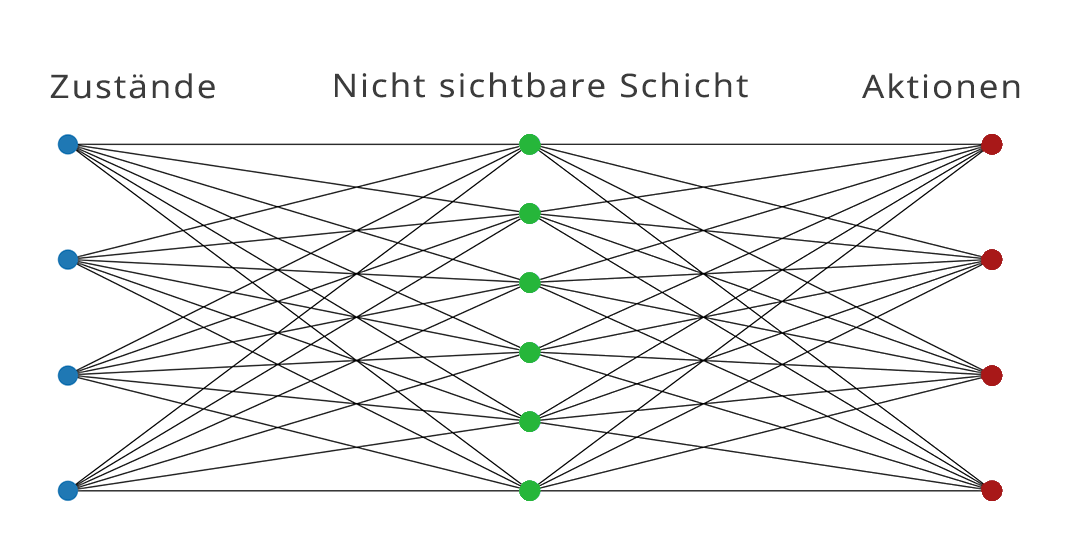
\includegraphics[width=\textwidth]{Figures/dn.png}
\caption{Einfaches euronales Netz}
\label{police}
\end{figure}

Die naheliegenste Möglichkeit ein neuronales Netz zu verwenden, ist die Funktion $Q(s, a)$ mit einem neuronalen Netz zu approximieren. Hierfür benutzen wir einfach einen versteckten Layer von Neuronen und realisieren dies mit PyTorch. Diese Layer werden Linear verbunden und mit der Relu-Aktivierungsfunktion versehen. Wir können dann den Fehler direkt mit der rechten Seite von \ref{SARSA} berechnen und an das Netz übergeben. Dazu benutzen wir den Adams-Optimierer.

\subsection{Generelle Boltzmann Maschine}
\label{subsec:bm}

Eine Boltzmann Maschine ist ein Ungerichtetes Probabilistisches Graphisches Modell \citep{DBLP:journals/jmlr/SallansH04}. Die Ecken des Graphen sind binäre Variablen und können die Werte 1 und 0 annehmen. Sie sind üblicherweise in sichtbare (v) und nicht-sichtbare (h) Variablen aufgeteilt. Die gewichteten Kanten sind paarweise symmetrische Interaktionen. Die Gewichte bestimmen die ``Energie'' von den Variablen. Allgemein können diese Gewichte zwischen allen Variablen auftauchen.

\begin{align}
	E(v,h) = - \sum_{k,i}w_{k,i}v_ih_k - \sum_{i < j}w_{ij}v_iv_j - \sum_{k<m}w_{km}h_kh_m \label{energie}
\end{align}

wobei i und j Indices über die sichtbaren Variaben und k und m Indices über die nicht-sichtbaren Variablen sind.
Wir wollen eine Energie-Funktion in Abhängigkeit der sichtbaren Variablen aufstellen:

\begin{align}
	F(v) = \sum_{h}\mathbb{P}(h|v)E(v,h) + \frac{1}{\beta} \sum_{h}\mathbb{P}(h|v)log(\mathbb{P}(h|v)) \label{F}
\end{align}

Dabei steht $\mathbb{P}(h|v)$ für die Wahrscheinlichkeit, dass die Variable h = 1 ist, mit dem gewählten Variblen v.
Um die erste Summe zu minimieren, werden möglichst viele Variablen auf 1 gesetzt, wo E(v,h) niedrig bzw. negativ ist und um die zweite Summe zu minimieren, soll die Wahrscheinlichkeitsverteilung von $\mathbb{P}$ eine hohe Entropie haben, das heißt, die Wahrscheinlichkeit soll entweder 1 oder 0 sein.
$\beta$ ist ein Parameter, den man wählen kann. Durch ihn kann man die Wirkung der zweiten Summe abschwächen.

Interessanterweise ist es recht einfach die Gewichte zu optimieren:

\begin{align}
	\frac{\partial F(v)}{\partial w_{ik}} = -v_i \langle h_k \rangle_{\mathbb{P}(h|v)} \label{update}
\end{align}

Dies liegt daran, dass die die Verteilung $\mathbb{P}(h|v)$ für F(v) minimal ist, sodass die Ableitung von F(v) in Abhängigkeit zu dieser Verteilung 0 ist. Für Details dazu siehe \citep{DBLP:journals/jmlr/SallansH04} Appendix A.

Wir können jetzt mit der Funktion F und der Optimierung der Gewichte eine Q-Funktion für einen Markov-Entscheidungsprozess mit einer Boltzmann Maschine darstellen. Die Zustände und Aktionen werden dabei zu einem Vektor vereinigt und bilden die sichtbaren Variablen. Es gilt:

\begin{align}
	F(v) = - Q(v)
\end{align}

\subsection{Beschränkte Boltzmann Maschine}
\label{subsec:rbm}

\begin{figure}[hbt!]
\centering
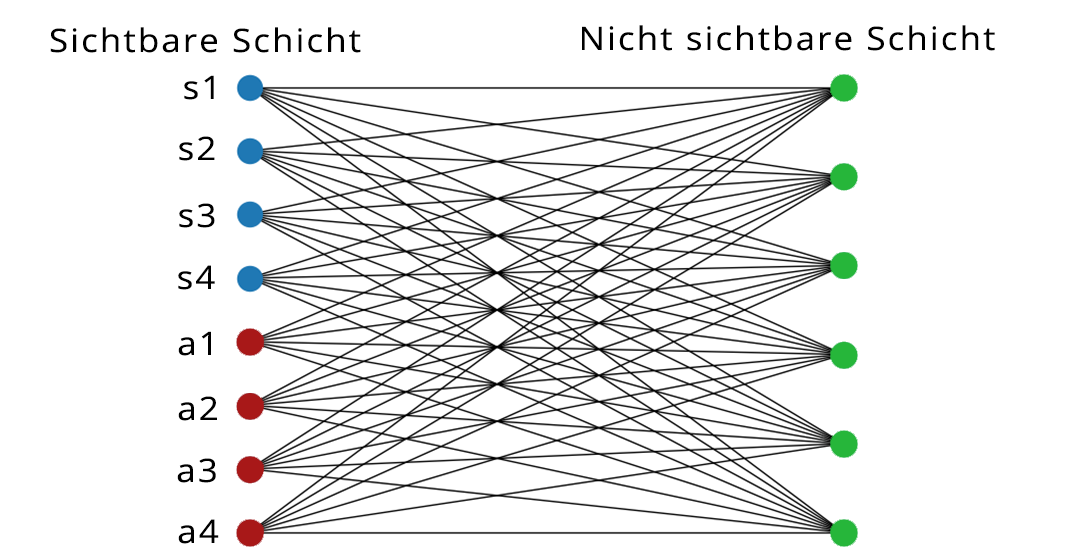
\includegraphics[width=\textwidth]{Figures/rbm.png}
\caption{Beschränkte Boltzmann Maschine}
\label{police}
\end{figure}

Eine beschränkte Boltzmann Maschine hat nur Gewichte zwischen sichtbaren und nicht-sichtbaren Variablen. So entsteht ein bipartiter Graph. Ansonsten bleibt alles gleich wie in (\ref{F}) und (\ref{update}). Die Energie E(v,h) reduziert sich dann auf:

\begin{align}
	E(v,h) = - \sum_{i,k}w_{i,k}v_ih_k
\end{align}

Q(s,a) können wir dann wie folgt zusammenfassen:

\begin{align*}
	Q(s,a) 	= 		&\sum_{h}\mathbb{P}(h|s,a)E(s,a,h) - \sum_{h}\mathbb{P}(h|s,a)log(\mathbb{P}(h|s,a))  \\
			=  	- 	&\sum_{k, } w_{i,k}s_i \langle h_k \rangle - \sum_{k,j} w_{j,k}a_j \langle h_k \rangle  \\
	- 	\frac{1}{\beta} 	&\sum_{k} \langle h_k \rangle log(\langle h_k \rangle) + (1 -  \langle h_k) \rangle log( (1 - \langle h_k \rangle) ) 
\end{align*}

wobei $\langle h_k \rangle$ mit der sigmoid Funktion berechnet wird:

\begin{align*}
	\langle h_k \rangle = \sigma (\sum_{i}w_{i,k}v_i)
\end{align*}

Dazu leiten wir uns aus (\ref{SARSA}) und (\ref{update}) die Regeln her, um nach jedem Schritt zu lernen:

\begin{align*}
	w_{sh} \: += \alpha ( r_n + \gamma Q(s_{n+1}, a_{n+1}) -  Q(s_n, a_n) ) s \langle h \rangle \\
	w_{ah} \: += \alpha ( r_n + \gamma Q(s_{n+1}, a_{n+1}) -  Q(s_n, a_n) ) a \langle h \rangle
\end{align*}

\subsection{Tiefe Boltzmann Maschine Resultate mit Quanten Annealing}
\label{subsec:dbm}

Die tiefe Boltzmann Maschine unterscheidet sich von der beschränkten Boltzmann Maschine dadurch, dass hier zusätzliche Verbindungen zwischen den Variablen der versteckten Schichten sind.

\begin{figure}[hbt!]
\centering
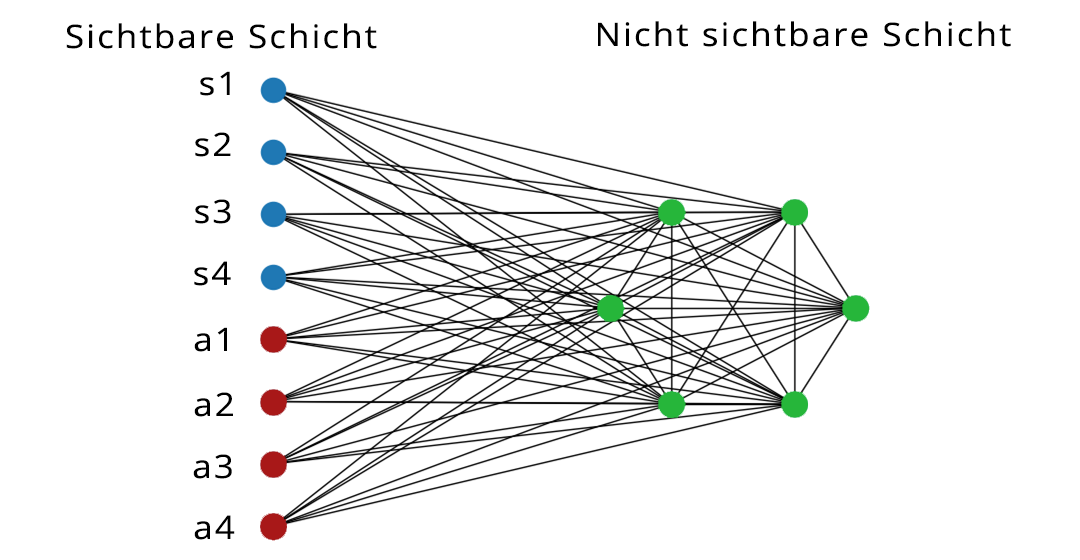
\includegraphics[width=\textwidth]{Figures/dbm.png}
\caption{Tiefe Boltzmann Maschine}
\label{police}
\end{figure}

Allgemein kann man eine tiefe Boltzmann Maschine auch mit mehreren versteckten Schichten aufbauen. Dann wandern die sichtbare Schicht mit den Aktionen auf die rechte Seite und die sichtbaren Schichten beeinflussen nur die benachbarten Variablen in den nicht-sichtbaren Schichten. Diese Variante wollen wir hier nicht betrachten.

Die Q-Funktion erweitert sich jetzt hier im Vergleich zur beschränkten Boltzmann Maschine um einen weiteren Term:

\begin{align}
	Q(s,a) =  	&- \sum_{k,i} w_{i,k}s_i \langle h_k \rangle  
				- \sum_{k,j} w_{j,k}a_j \langle h_k \rangle   
				- \sum_{k,m}w_{km} \langle h_k h_m \rangle \label{Qdbm1}   \\  
				&-  \frac{1}{\beta} \sum_{k} \langle h_k \rangle log(\langle h_k \rangle) + (1 -  \langle h_k) \rangle log( (1 - \langle h_k \rangle) )  \label{Qdbm2}
\end{align}

und auch die Update-Regel bekommt einen weiteren Teil:

\begin{align*}
	w_{sh} \: 			&+= \alpha ( r_n + \gamma Q(s_{n+1}, a_{n+1}) -  Q(s_n, a_n) ) s \langle h \rangle \\
	w_{ah} \: 			&+= \alpha ( r_n + \gamma Q(s_{n+1}, a_{n+1}) -  Q(s_n, a_n) ) a \langle h \rangle \\
	w_{hh^{\prime}} \: 	&+= \alpha ( r_n + \gamma Q(s_{n+1}, a_{n+1}) -  Q(s_n, a_n) ) \langle h h^{\prime} \rangle 
\end{align*}

Jetzt kommt der spannende Teil. Die freie Energie der tiefen Boltzmann Maschine kann aus (\ref{energie}) abgeleitet wie folgt berechnet werden:

\begin{align}
	E_v(h) = - \sum_{k,i}w_{k,i}v_ih_k - \sum_{k<m}w_{km}h_kh_m \label{energiedbm}
\end{align}

Dabei sind die sichtbaren Schichten v jetzt feste Parameter und nur noch h sind freie Variablen. Da $\langle h \rangle$ binäre Variablen sind und wir die Gesamtenergie minimieren wollen, handelt es sich hier also um ein quadratisches, binäres Optimierungsproblem kurz QUBO. Dieses können wir mit Hilfe von Annealing lösen oder auch mit Hilfe von einem Quantencomputer mit QAOA oder mit adiabatischen Quantencomputern. Wir interessieren uns vor allem für Quanten-Annealing, einer Unterform von adiabatischen Quantencomputern, welches von DWave erforscht wird. Wir haben dabei einen vollvernetzten Graphen mit so vielen Variablen, wie wir Neuronen in der versteckten Schicht haben. Hier kann der DWave bekanntlich auch Probleme mit z.B. 16 Variablen gut lösen. Da wir aber in unseren Tests für einen Testlauf meistens 10 000 Spiele auf dem Frozen Lake spielen wollen und für jeden einzelnen Zug 8 QUBO's lösen müssen, verwenden wir hier simuliertes Quanten Annealing.

Eine naheliegende Idee wäre jetzt (\ref{Qdbm1}) mit der durchschnittlichen Energie zu ersetzen, die wir in unserem QUBO Problem durch den Hamiltonian ausgerechnet haben. Diese bekommen wir vom simulierten Annealing (wir benutzen dafür eine Library von DWave) zurück und können diese gleich einsetzen.
Allerdings ist die durchschnittliche Energie nicht identisch mit der Energie, die wir aus den verstecken Variablen h berechnen. Der Grund dafür sind die quadratischen Terme im QUBO. Dazu ein kleines Beispiel:

Sei ein QUBO gegeben, durch zwei Variablen die mit einer Kante verbunden sind. Diese Kante hat den Wert -1. Führen wir jetzt zwei Annealing Durchläufe aus, bekommen wir zum Beispiel die Ergebnisse (1,1) und (0,0). Damit berechnen wir die Aktivierung von den versteckten Variablen mit:

\begin{align}
	\frac{(1, 1) + (0, 0)}{2} = (0.5, 0.5)
\end{align}

Es ergibt sich mit (\ref{Qdbm1}) ohne die Entropy die Energie:

\begin{align}
	0.5 * 0.5 * -1 = -0.25
\end{align}

Im Vergleich dazu, hat das erste Ergebnis (1,1) die Energie -1 und das zweite Ergebnis (0,0) die Energie 0 und damit wäre die durchschnittliche Energie -0.5.

Das heißt wir bekommen mit der durchschnittlichen Energie unserer Messergebnisse ein ähnliches aber leicht verschiedenes Ergebniss zu (\ref{Qdbm1}), welches die freie Energie der Boltzmann Maschine beschreibt. In verschiedenen Tests zeigte sich auch, dass der Algorithmus mit der durchschnittlichen Energie aus den Messergebnissen ähnliche Ergebnisse liefert, jedoch ein wenig schlechter als mit der direkten Berechnung durch  (\ref{Qdbm1}). Wir wollen daher die Variante mit der durchschnittlichen Energie im weiteren nicht näher betrachten.

\subsection{Quanten Annealing}
\label{subsec:QA}

Wir können ein Optimierungsproblem als ein System beschreiben, sodass die minimale Energie des Systems der Lösung von unserem Optimierungssystem entspricht.
Für das Quanten Annealing können wir hier das Ising Problem verwenden. Ein QUBO ist allerdings äquivalent dazu und wir können ein QUBO in ein Ising Problem umwandeln.
So ein Ising Problem stellen wir dann mit einem Hamiltonian dar, welcher die Energie des Systems beschreibt.

Nach dem Adiabatischen Theorem gilt: Wenn sich das System im Grundzustand des ersten Hamiltonians befindet und sich dann adiabatisch langsam genug zeitlich verändert, wird es sich danach im Grundzustand des zweiten Hamiltonians befinden. 

Der erste Hamiltonian $H_{0}$ ist dabei das sogenannte Transverse Feld, dessen Energieminimum eine Superposition von allen Qubits ist. 
Der zweite Hamiltonian $H_{1}$ ist dabei ein von uns aufgestellter Hamiltonian, dessen Energieminimum der Lösung von unserem Optimierungsproblem entspricht.

\begin{equation}
    H_{0} = - \sum_{i} \sigma^{x}_{i}
 \end{equation}
\begin{equation}
    H_{1} = \sum_{i, j} J_{ij} \sigma^{z}_{i}  \sigma^{z}_{j}  + \sum_{i} h_i \sigma^{z}_{i}
 \end{equation}

Wir können dann einen zeitabhängigen Hamiltonian angeben, der eine Mischung vom ersten und zweiten Hamiltonian darstellt:

\begin{equation}
    H(t) = (1-t) H_{0} + t H_{1} , t \in [0,1]
 \end{equation}

Wenn wir diesen zeitlichen Prozess, den wir Annealing nennen, langsam genug durchführen, kommen wir am Schluss bei t = 1 sicher in der minimalen Energie des $H_{1}$ Hamiltonians an und haben damit unser Optimierungsproblem gelöst.
Wie langsam dieser Prozess sein muss, hängt dabei vom minimalen Unterschied (Gap) des niedriegsten Energie Niveaus zum ersten angeregten Energienieveau ab.

Wir benutzen Quanten Annealing oder simuliertes Quanten Annealing um eine Lösung von (\ref{energiedbm}) zu finden. Allerdings haben wir hier eine Besonderheit, wir wollen nicht unbedingt immer die beste Lösung finden, denn dann wären unsere versteckten Variablen immer entweder 0 oder 1, wie die binären Variablen in der Lösung vom QUBO. Stattdessen führen wir mehrere Durchläufe vom Annealing Prozess durch und wählen dabei die Annealing Zeit so kurz, das wir verschiedene Lösungen finden. So können wir den Durchschnitt der Lösungen berechnen und bekommen so weichere Aktivierungen für unsere versteckten Variablen, die auch zwischen 0 und 1 liegen können.

Wie wir dann auch in unseren Experimenten sehen können, brauchen wir (\ref{Qdbm2}) für diese Version nicht mehr, da wir mit den Parametern im simulierten Annealing schon steuern können, wir sehr die Variablen richtung 0 oder 1 tendieren. Damit wird die Zeile einfach überflüssig und wir sehen auch in den Experimenten, dass dieser Term dafür sorgt, dass wir die Lösungen langsamer finden.

\section{Resultate}
\label{sec:res}

\subsection{Prinzipien des Testens}
\label{subsec:Prinzipien}

Wir wollen hier festlegen, wie wir testen, was wir testen, wie die Ergebnisse dargestellt und wie sie zu bewerten sind.

Als erstes wollen wir bei jeder Methode die verschiedenen Parameter und ihre Auswirkungen auf die Lösungen testen. Dabei beschränken wir uns hauptsächlich auf ein 3x3 Feld mit der $\epsilon$-Greedy-Methode, da wir hier weniger Rechenzeit brauchen und mit jeder Methode richtige Lösungen finden können. Wenn wir bereits gute Parameter einer Methode gefunden haben, ist es auch interessant kompliziertere Spielfelder auszuprobieren. Bei sehr großen Spielfeldern stößt irgendwann die $\epsilon$-Greedy-Methode an ihre Grenzen, da wir hier mit einer zufälligen Police am Anfang nicht mehr das Ziel finden können. 

\begin{figure}[H]
\centering
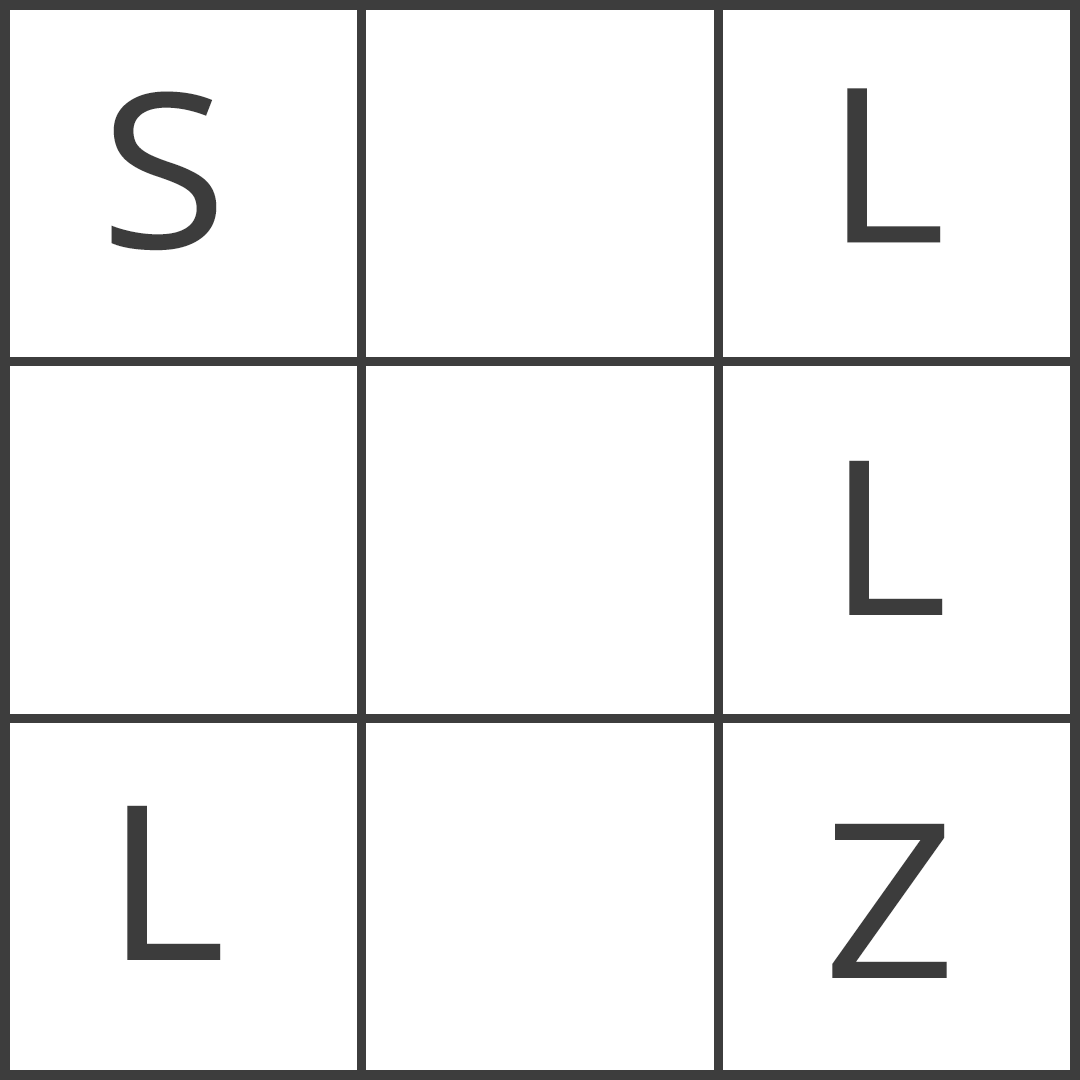
\includegraphics[width=\textwidth]{Figures/Intermediate.png}
\caption{3x3 Feld}
\label{advanced}
\end{figure}

Hier gibt es zwei Möglichkeiten, die erste ist, dass wir unser Startfeld in die Nähe des Ziels setzen und so lernen. Dann können wir ohne das Netz zurückzusetzen, das Startfeld weiter vom Ziel entfernen und von dort weiter lernen. So können wir das Startfeld in mehreren Schritten zur eigentlichen Startposition bewegen und haben so eine Chance, die richtige Lösung zu finden. Interessant ist hier, wie stabil die Methoden mit den bis jetzt gelernten Policen umgehen und etwas dazulernen können, ohne altes zu verlernen. 

Die zweite Möglichkeit ist, komplett von der $\epsilon$-Greedy-Methode abzusehen und eine Schleife über alle Felder zu machen und für jedes Feld jede Aktion zu testen und daraus zu lernen. Das funktioniert besser, braucht aber für große Spielfelder sehr viel Rechenzeit, bis wir die richtige Lösung gefunden haben.

Die Resultate lassen wir durch einen Graphen anzeigen. Bei der $\epsilon$-Greedy-Methode stehen auf der y-Achse die durchschnittlichen Punkte von 100 Spielen. Bei der Schleife über alle Felder dagegen, betrachten wir, von wie vielen Feldern wir die richtige Lösung finden können und zeichnen dies auf der y-Achse auf.

\subsection{Q-Tabelle Resultate}
\label{subsec:Q-Tabelle_r}

Die Q-Tabelle findet immer eine passende Lösung, wenn durch zufällige Aktionen zumindestens einmal die Lösung gefunden werden kann.

Testen wir erst mit Standardparametern.
Der blaue Graph ist hier übrigens  $\epsilon$. In den meisten Vergleichen, wenn wir verschiedene Parameter testen wollen, lassen wir  $\epsilon$ weg. Die  $\epsilon$ Kurve sieht aber immer gleich aus, es sei denn, wenn wir verschiedene Startfelder nacheinander wählen.

\begin{figure}[H]
\centering
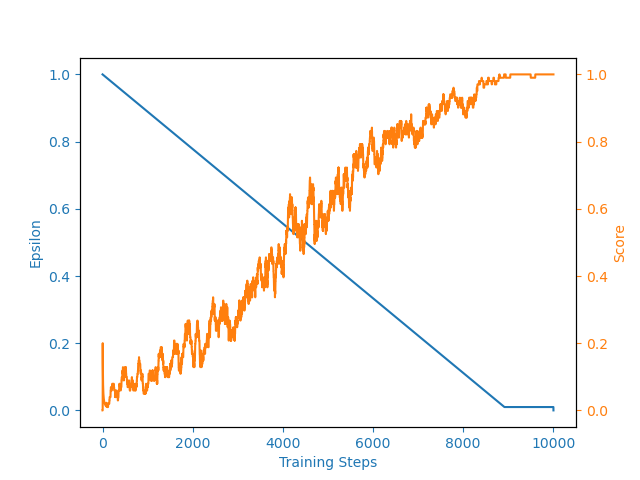
\includegraphics[width=\textwidth]{Figures/q_table_3x3.png}
\caption{3x3 Q-Tabelle}
\label{q1}
\end{figure}

\begin{figure}[H]
\centering
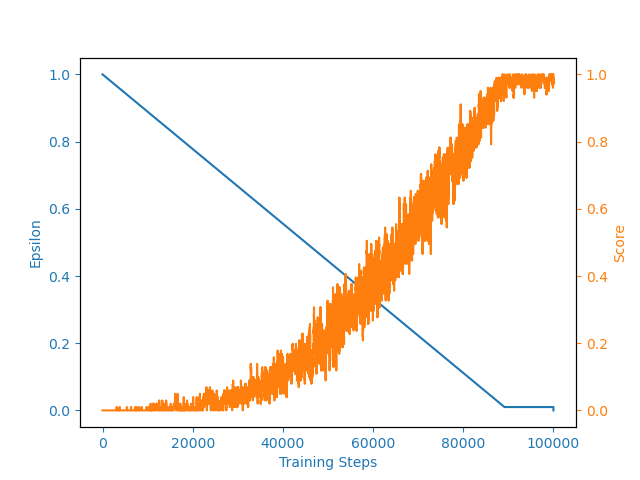
\includegraphics[width=\textwidth]{Figures/q_table_5x5.png}
\caption{5x5 Q-Tabelle}
\label{q2}
\end{figure}

\begin{figure}[H]
\centering
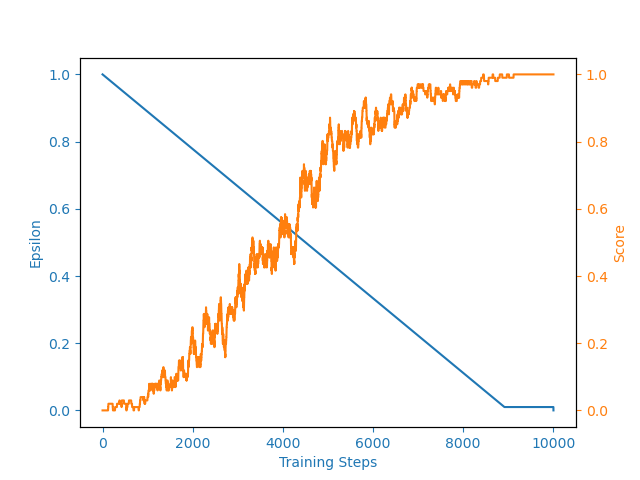
\includegraphics[width=\textwidth]{Figures/q_table_8x8.png}
\caption{8x8 Q-Tabelle}
\label{q3}
\end{figure}

Das 5x5 Feld ist sehr voll mit Löchern, daher sorgen hier geringe $\epsilon$ immer noch für einige falsche Züge und damit für niedrigere Punkte.

Allerdings fällt auf, dass wir bei dem 5x5 Feld schon die Anzahl der Spiele deutlich erhöhen müssen, um überhaupt das Ziel zu finden. Eine elegantere Alternative ist, die Q-Tabelle nicht mit 0 zu initialisieren, sondern z.B. mit 0.5. Es passiert dann Folgendes: Sobald der Agent eine Aktion macht, die keine Belohnung bekommt, wird der Wert der Q-Tabelle reduziert. Daher macht der Agent beim nächsten Mal eine andere Aktion. So werden vor allem weit entfernte Ecken des Spielfeldes erreicht.

Im Folgenden die Ergebnisse mit den Initialwerten 0, 0.5 und 1:

\begin{figure}[H]
\centering
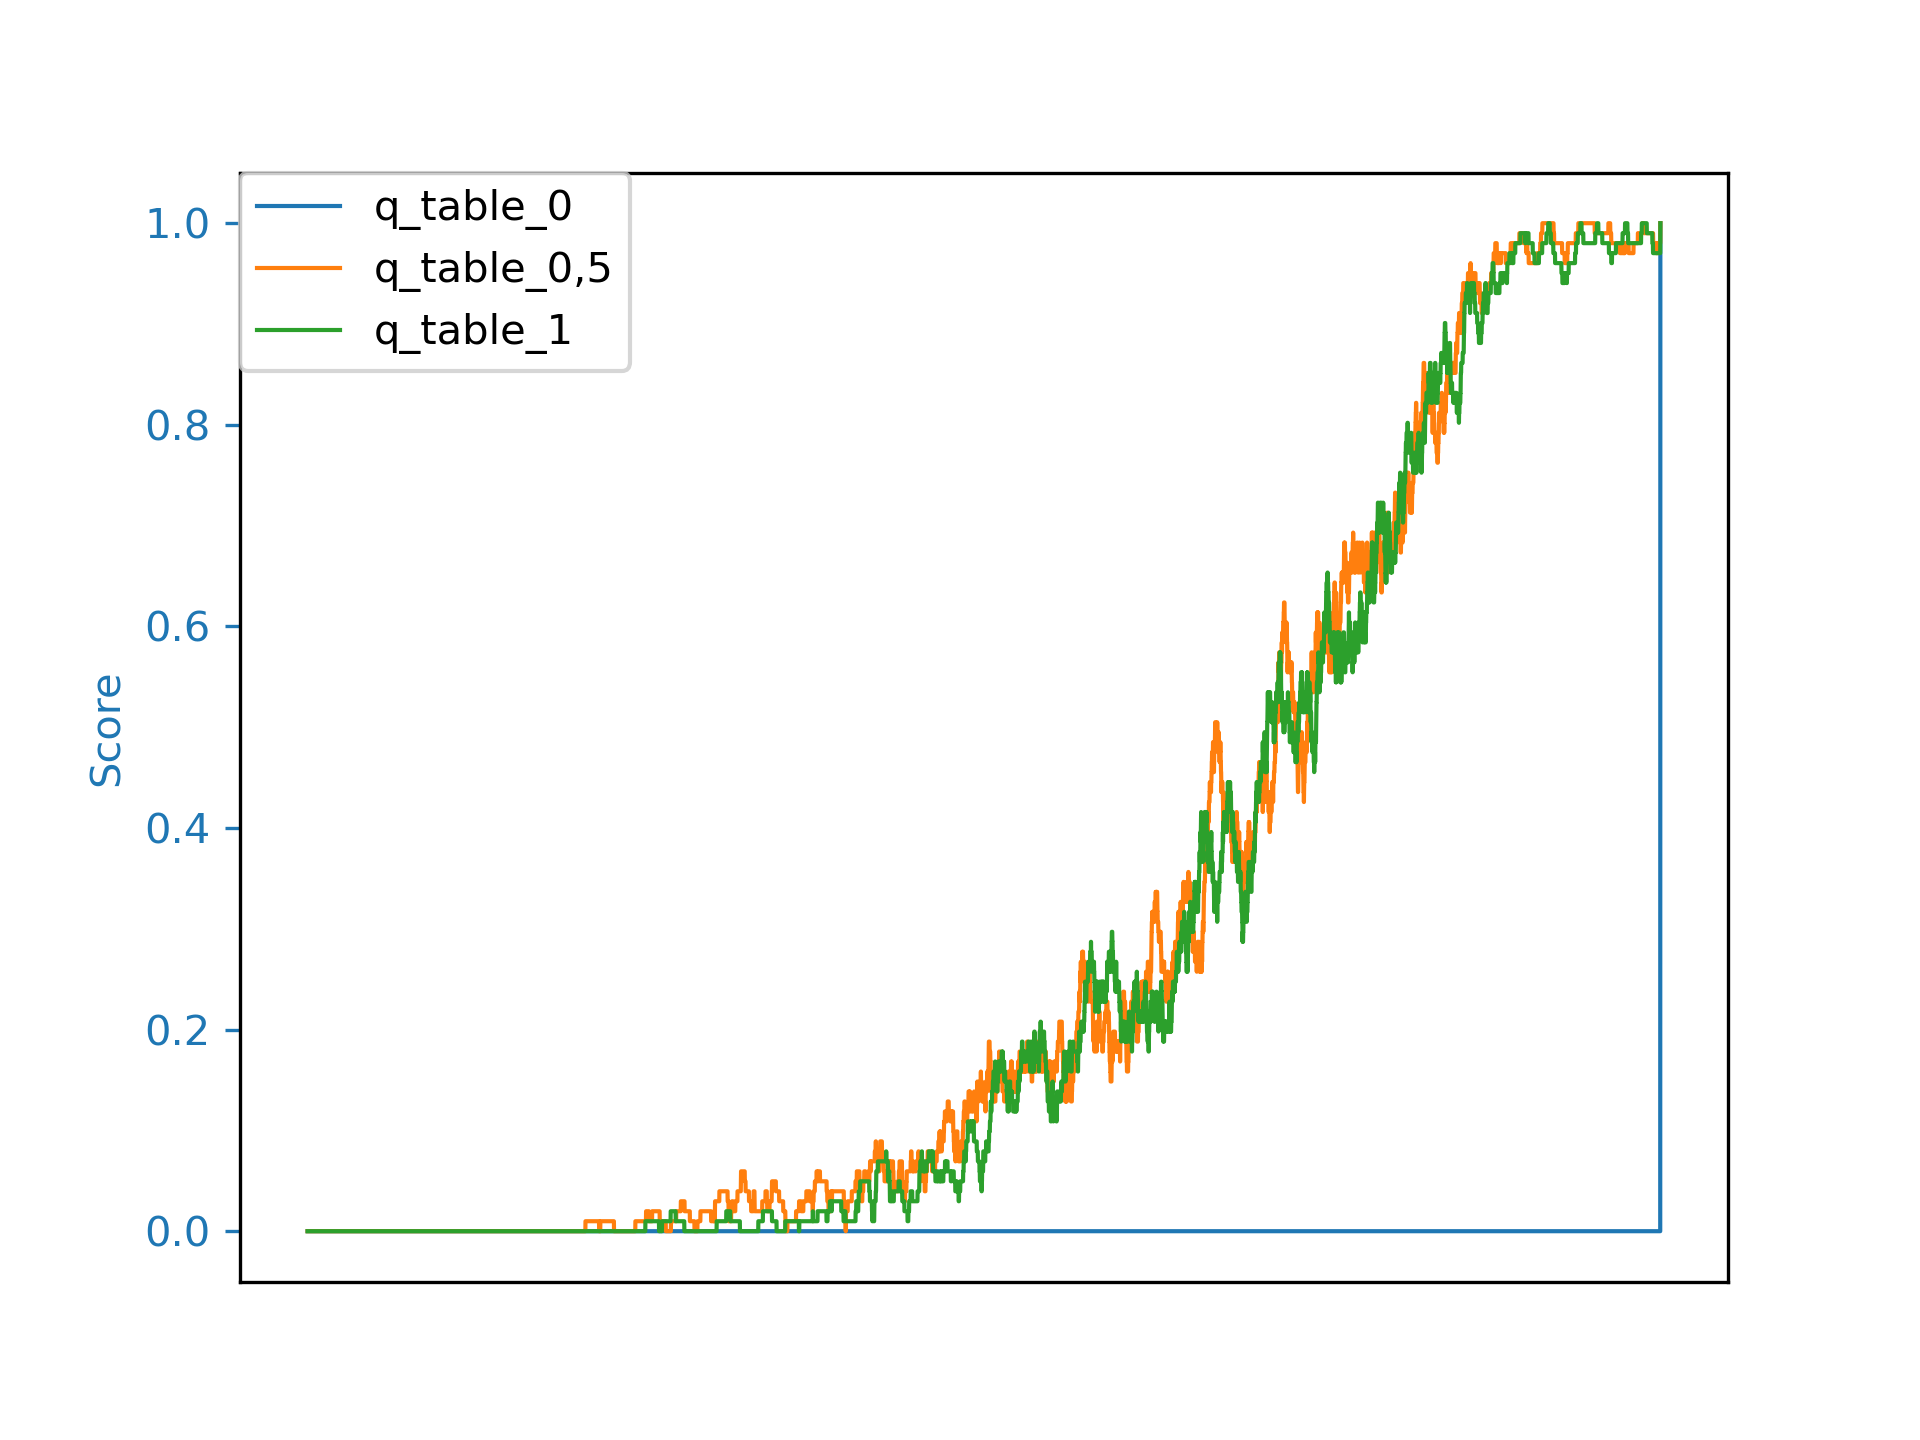
\includegraphics[width=\textwidth]{Figures/5x5_q_table_0_q_table_0,5_q_table_1.png}
\caption{5x5 Q-Tabelle}
\label{q2}
\end{figure}

Während der Agent mit dem Initialwert 0 das Ziel nie findet und garnicht anfangen kann zu lernen, finden die beiden anderen Versionen die Lösung extrem schnell.

\subsection{Einfaches neuronales Netz Resultate}
\label{subsec:dn_r}

Hier wollen wir als erstes testen, wie viele Neuronen wir in der versteckten Schicht brauchen, um überhaupt richtige Ergebnisse zu erzielen. Dies testen wir in dem kleinsten 2x2 Spielfeld.

\begin{figure}[H]
\centering
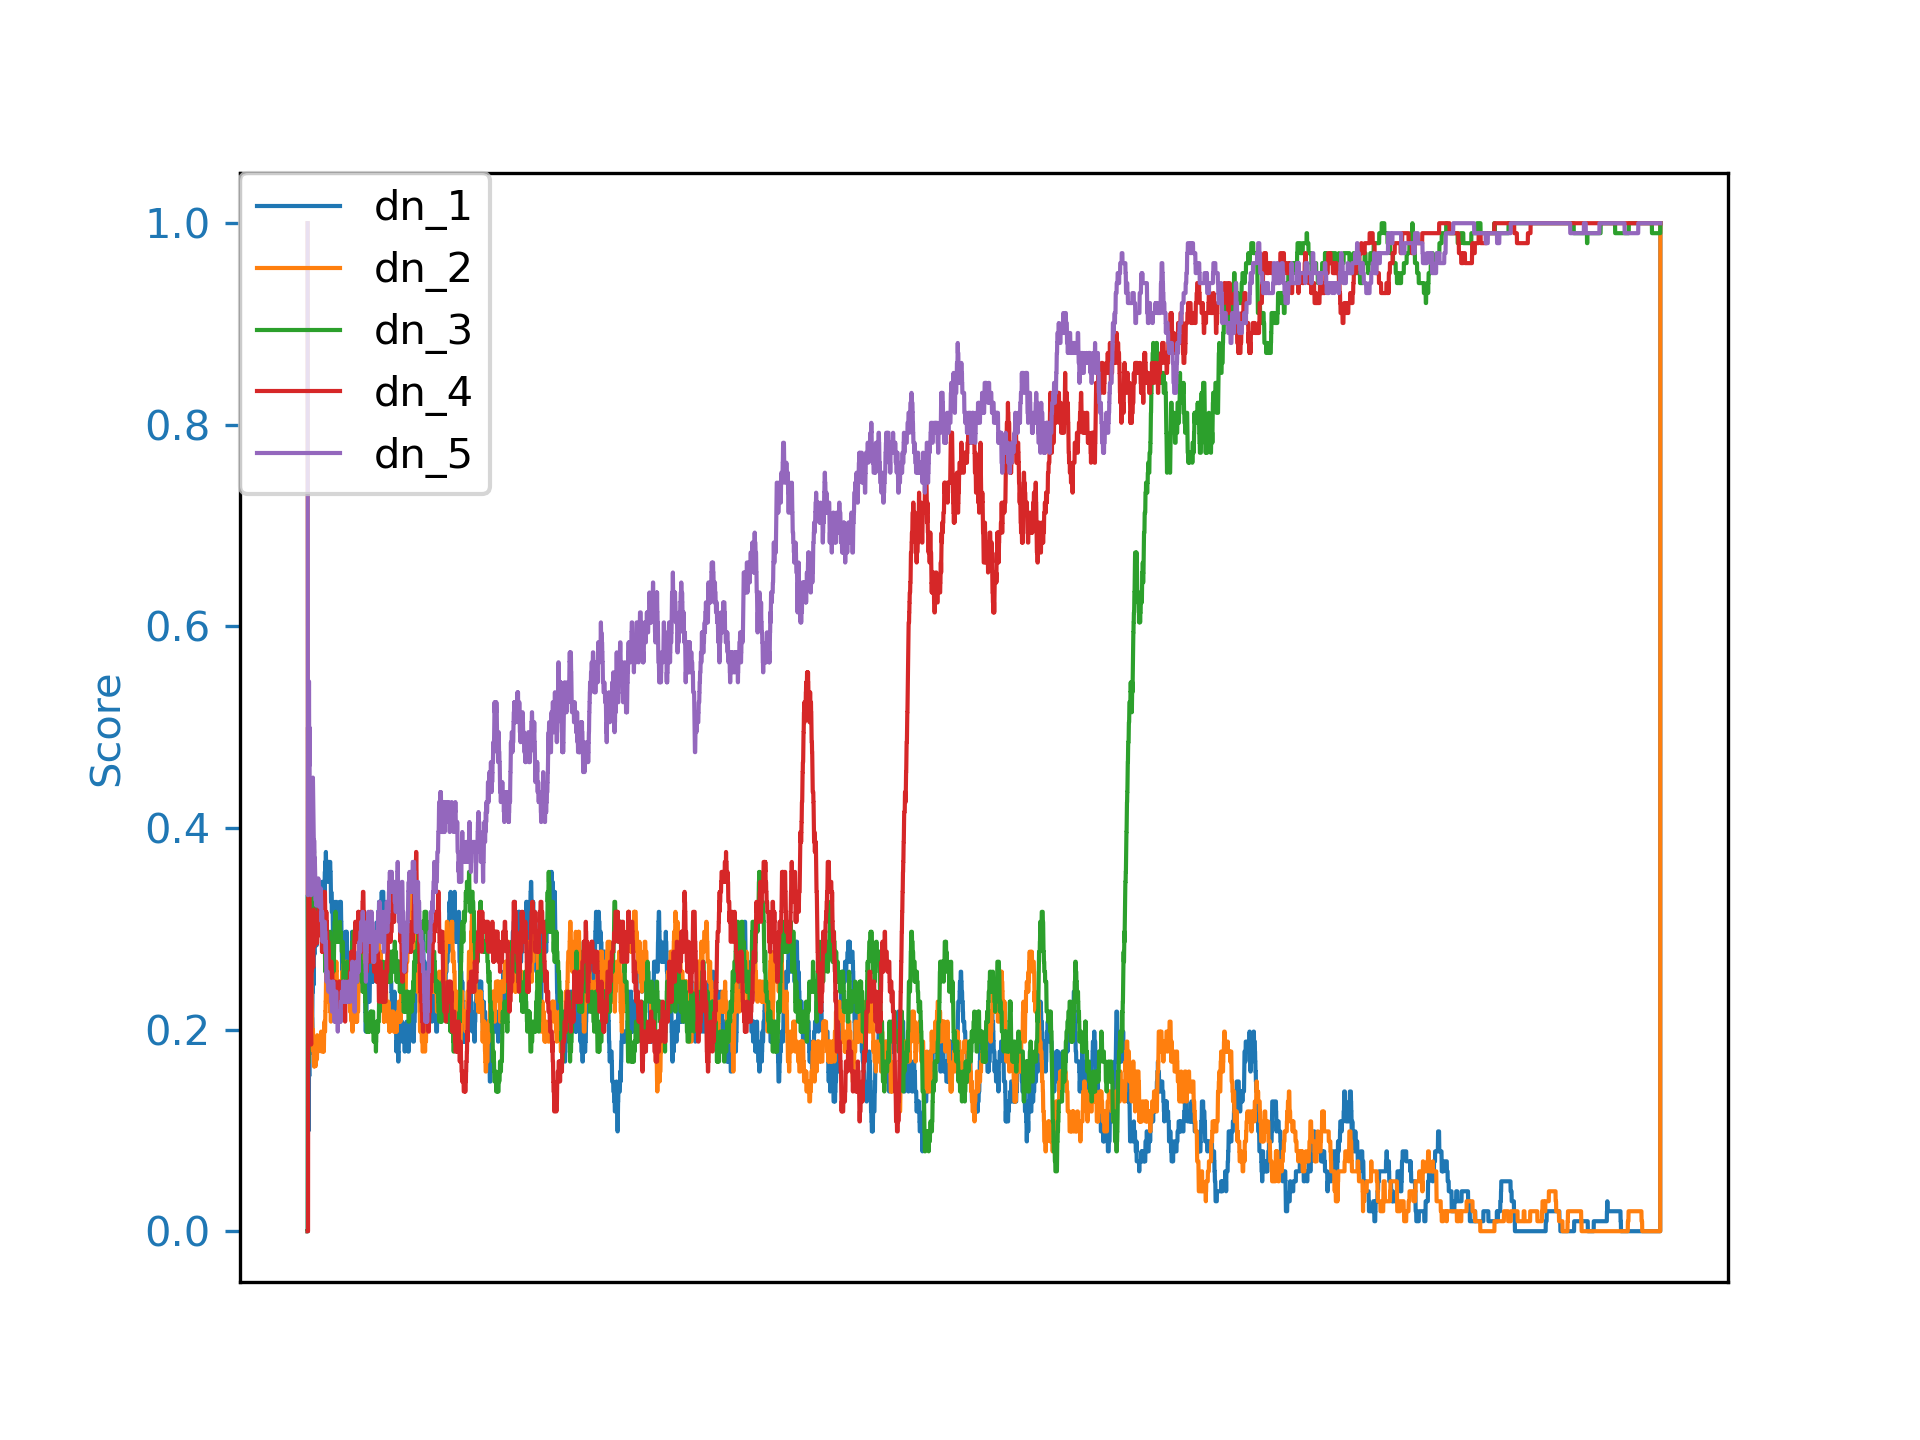
\includegraphics[width=\textwidth]{Figures/2x2_dn_1_dn_2_dn_3_dn_4_dn_5.png}
\caption{2x2 Neuronales Netz: Neuronen}
\label{dn1}
\end{figure}

Wir brauchen also mindestens 3 Neuronen, um auf die richtige Lösung zu kommen. Das ist interessant, da wir 4 Aktionen und 4 Zustände haben. Wir können das Problem also mit weniger Neuronen als möglichen Aktionen lösen. Ab 5 Neuronen gibt es keine klaren Unterschiede mehr bei dem kleinen Spielfeld.

Beim 3x3 Feld brauchen wir gleich deutlich mehr Neuronen. Zwischen 8 und 64 Neuronen bekommen wir richtige Ergebnisse.

\begin{figure}[H]
\centering
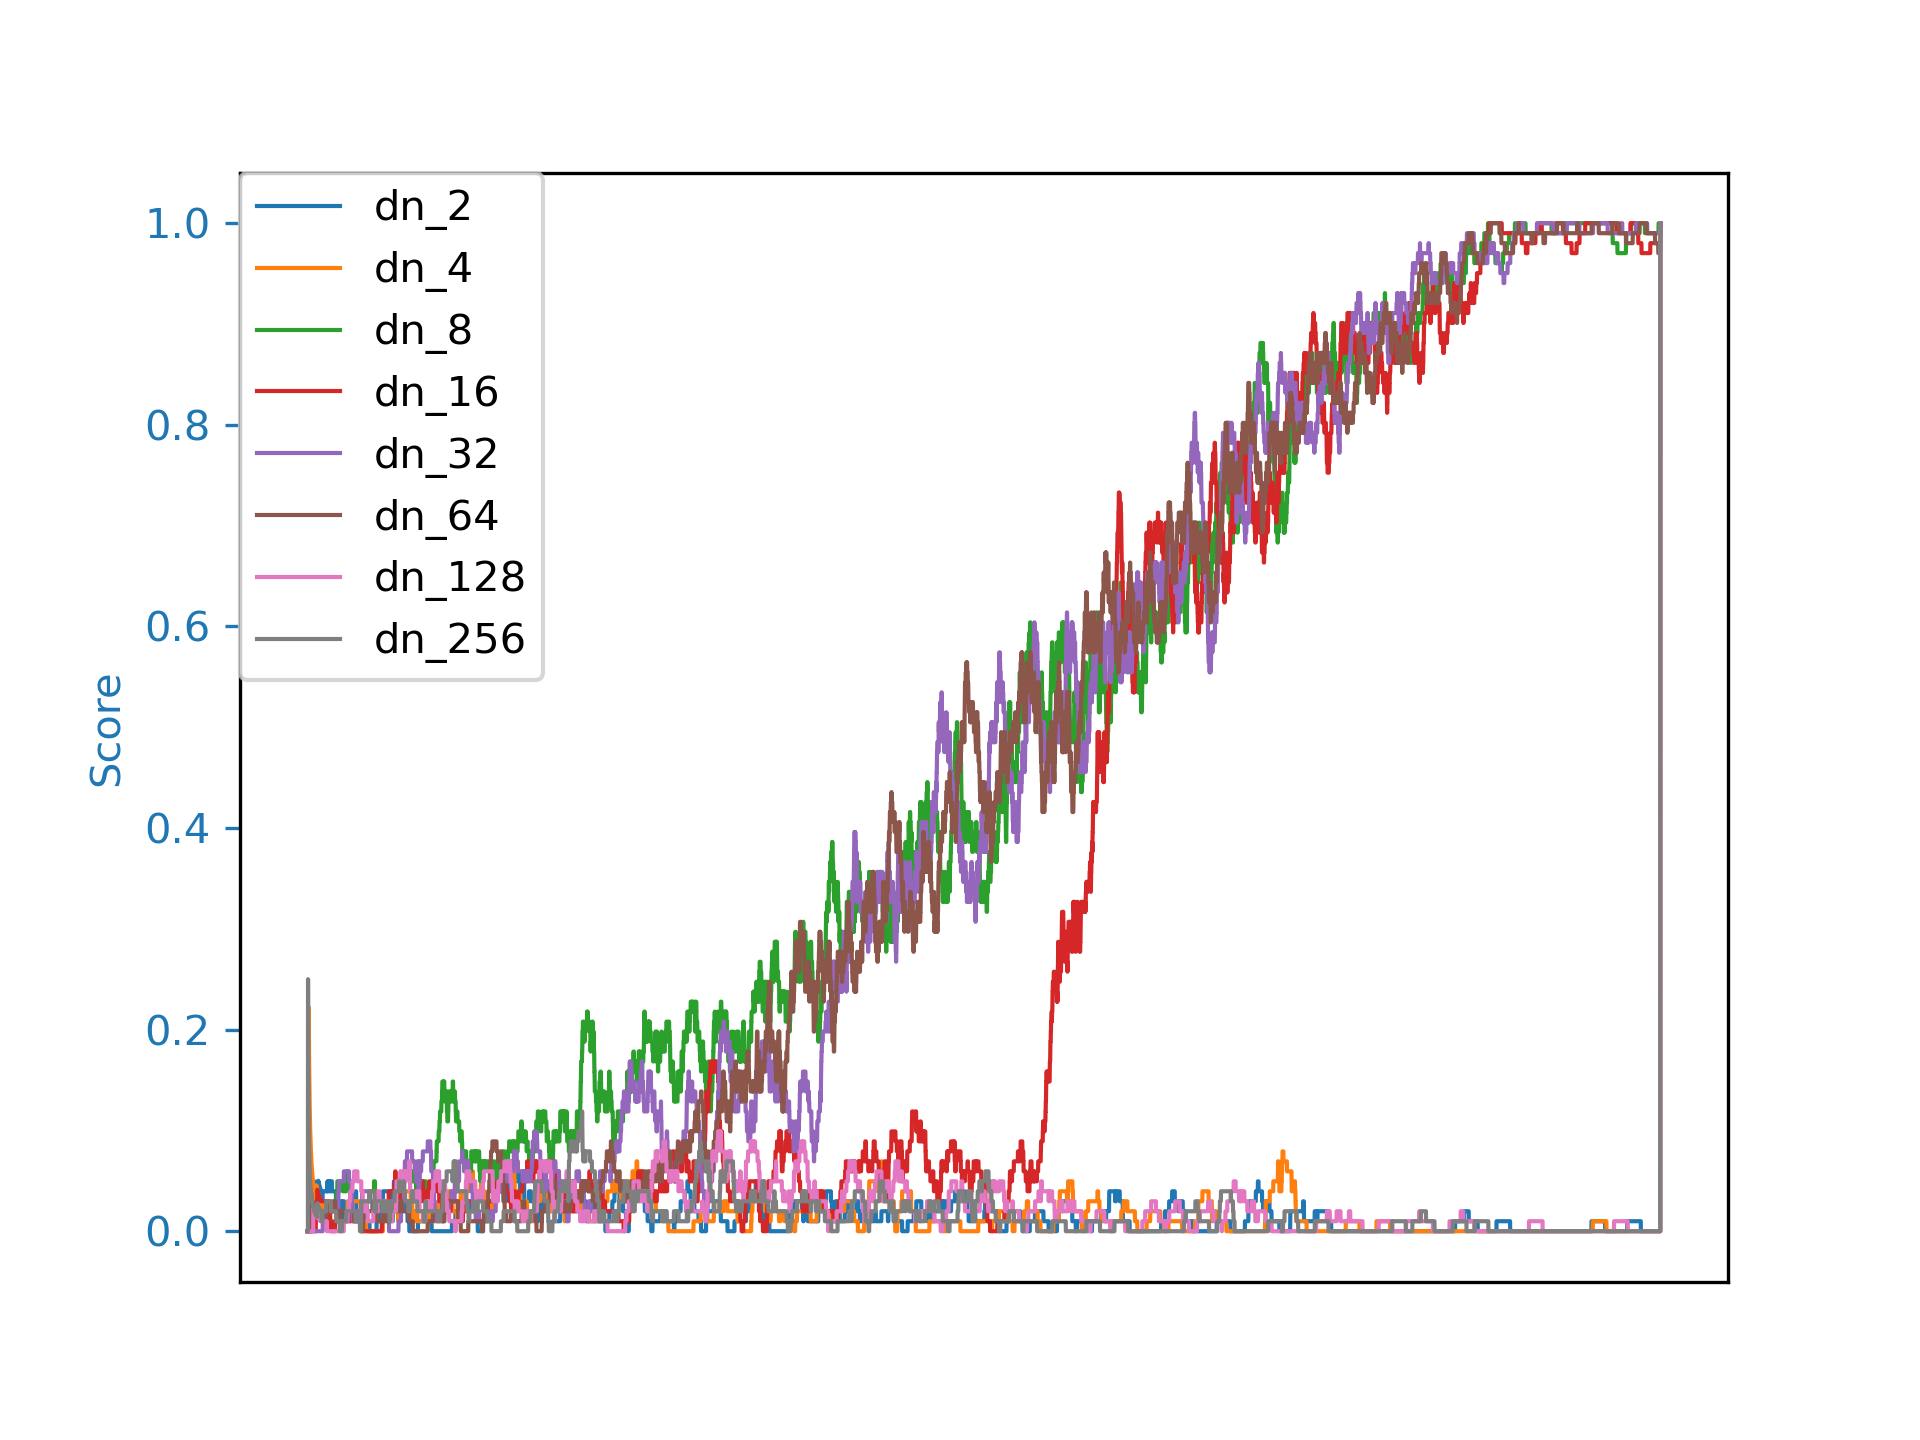
\includegraphics[width=\textwidth]{Figures/3x3_dn_2_dn_4_dn_8_dn_16_dn_32_dn_64_dn_128_dn_256.png}
\caption{3x3 Neuronales Netz: Neuronen}
\label{dn2}
\end{figure}

Als nächstes testen wir mit 16 Neuronen weiter und vergleichen verschiedene Werte für $\gamma$.

\begin{figure}[H]
\centering
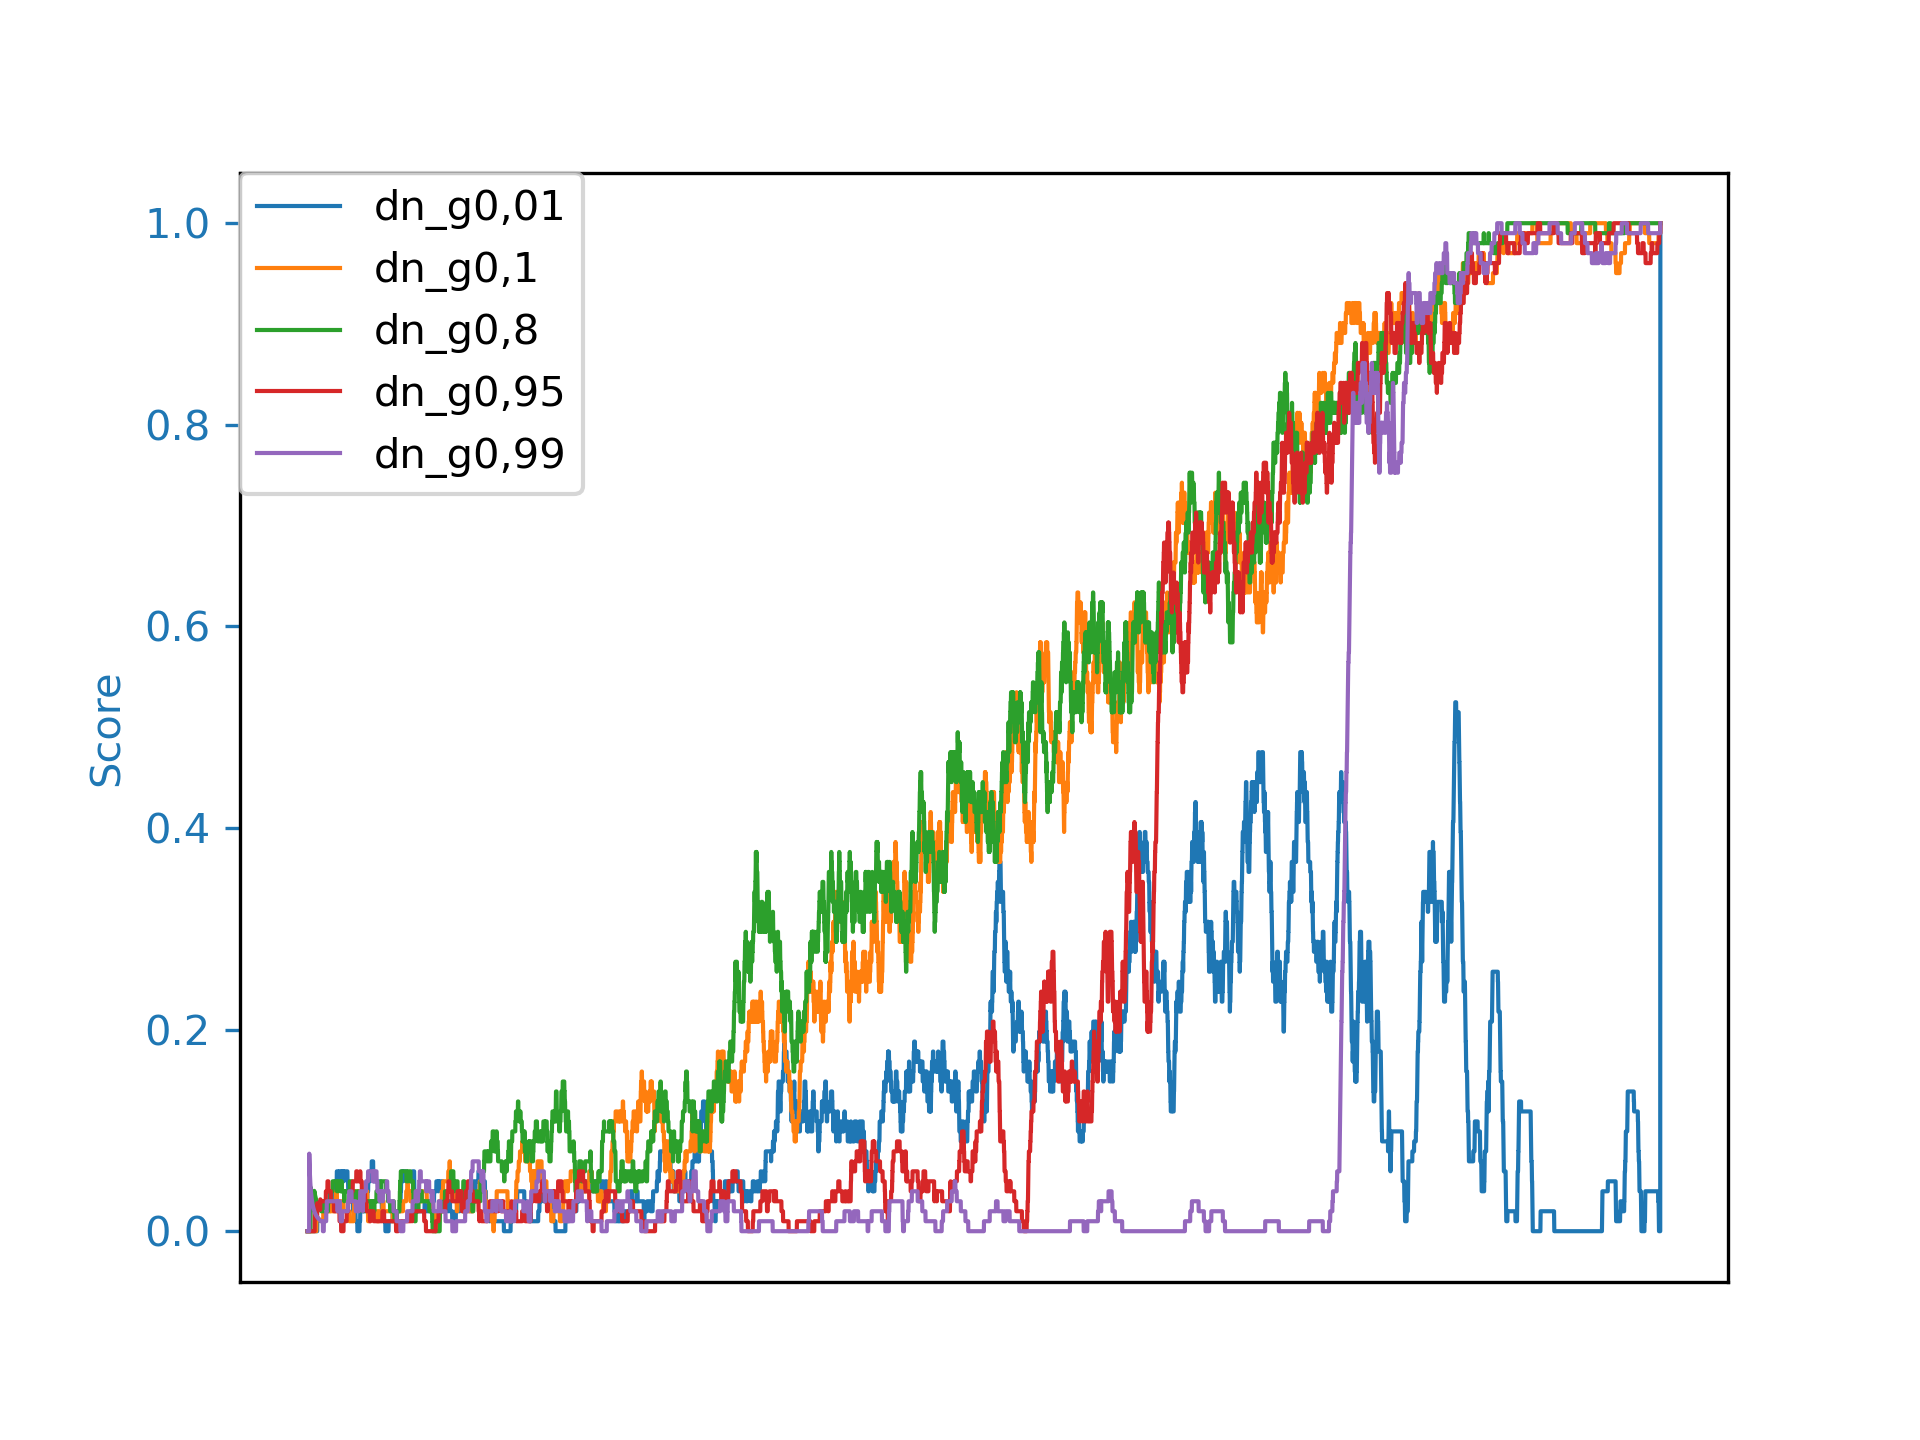
\includegraphics[width=\textwidth]{Figures/3x3_dn_g0,01_dn_g0,1_dn_g0,8_dn_g0,95_dn_g0,99.png}
\caption{3x3 Neuronales Netz: $\gamma$}
\label{dn3}
\end{figure}

Am besten haben hier die Werte 0,1 und 0,8 für $\gamma$ funktioniert. Wir bleiben also im weiteren bei dem Wert 0,8. Dieser wird auch häufig in der Literatur verwendet. Behalten wir aber im Auge, das eventuell niedrigere Werte besser funktionieren könnten.

Zuletzt wollen wir die Lernrate testen. Eine hohe Lernrate kann dazu führen, dass das Netz hin und her schwankt und sich nicht einpendelt. Eine zu niedrige Lernrate kann dazu führen, dass die 10000 Spiele nicht ausreichen, um das richtige Ergebnis zu lernen.

\begin{figure}[H]
\centering
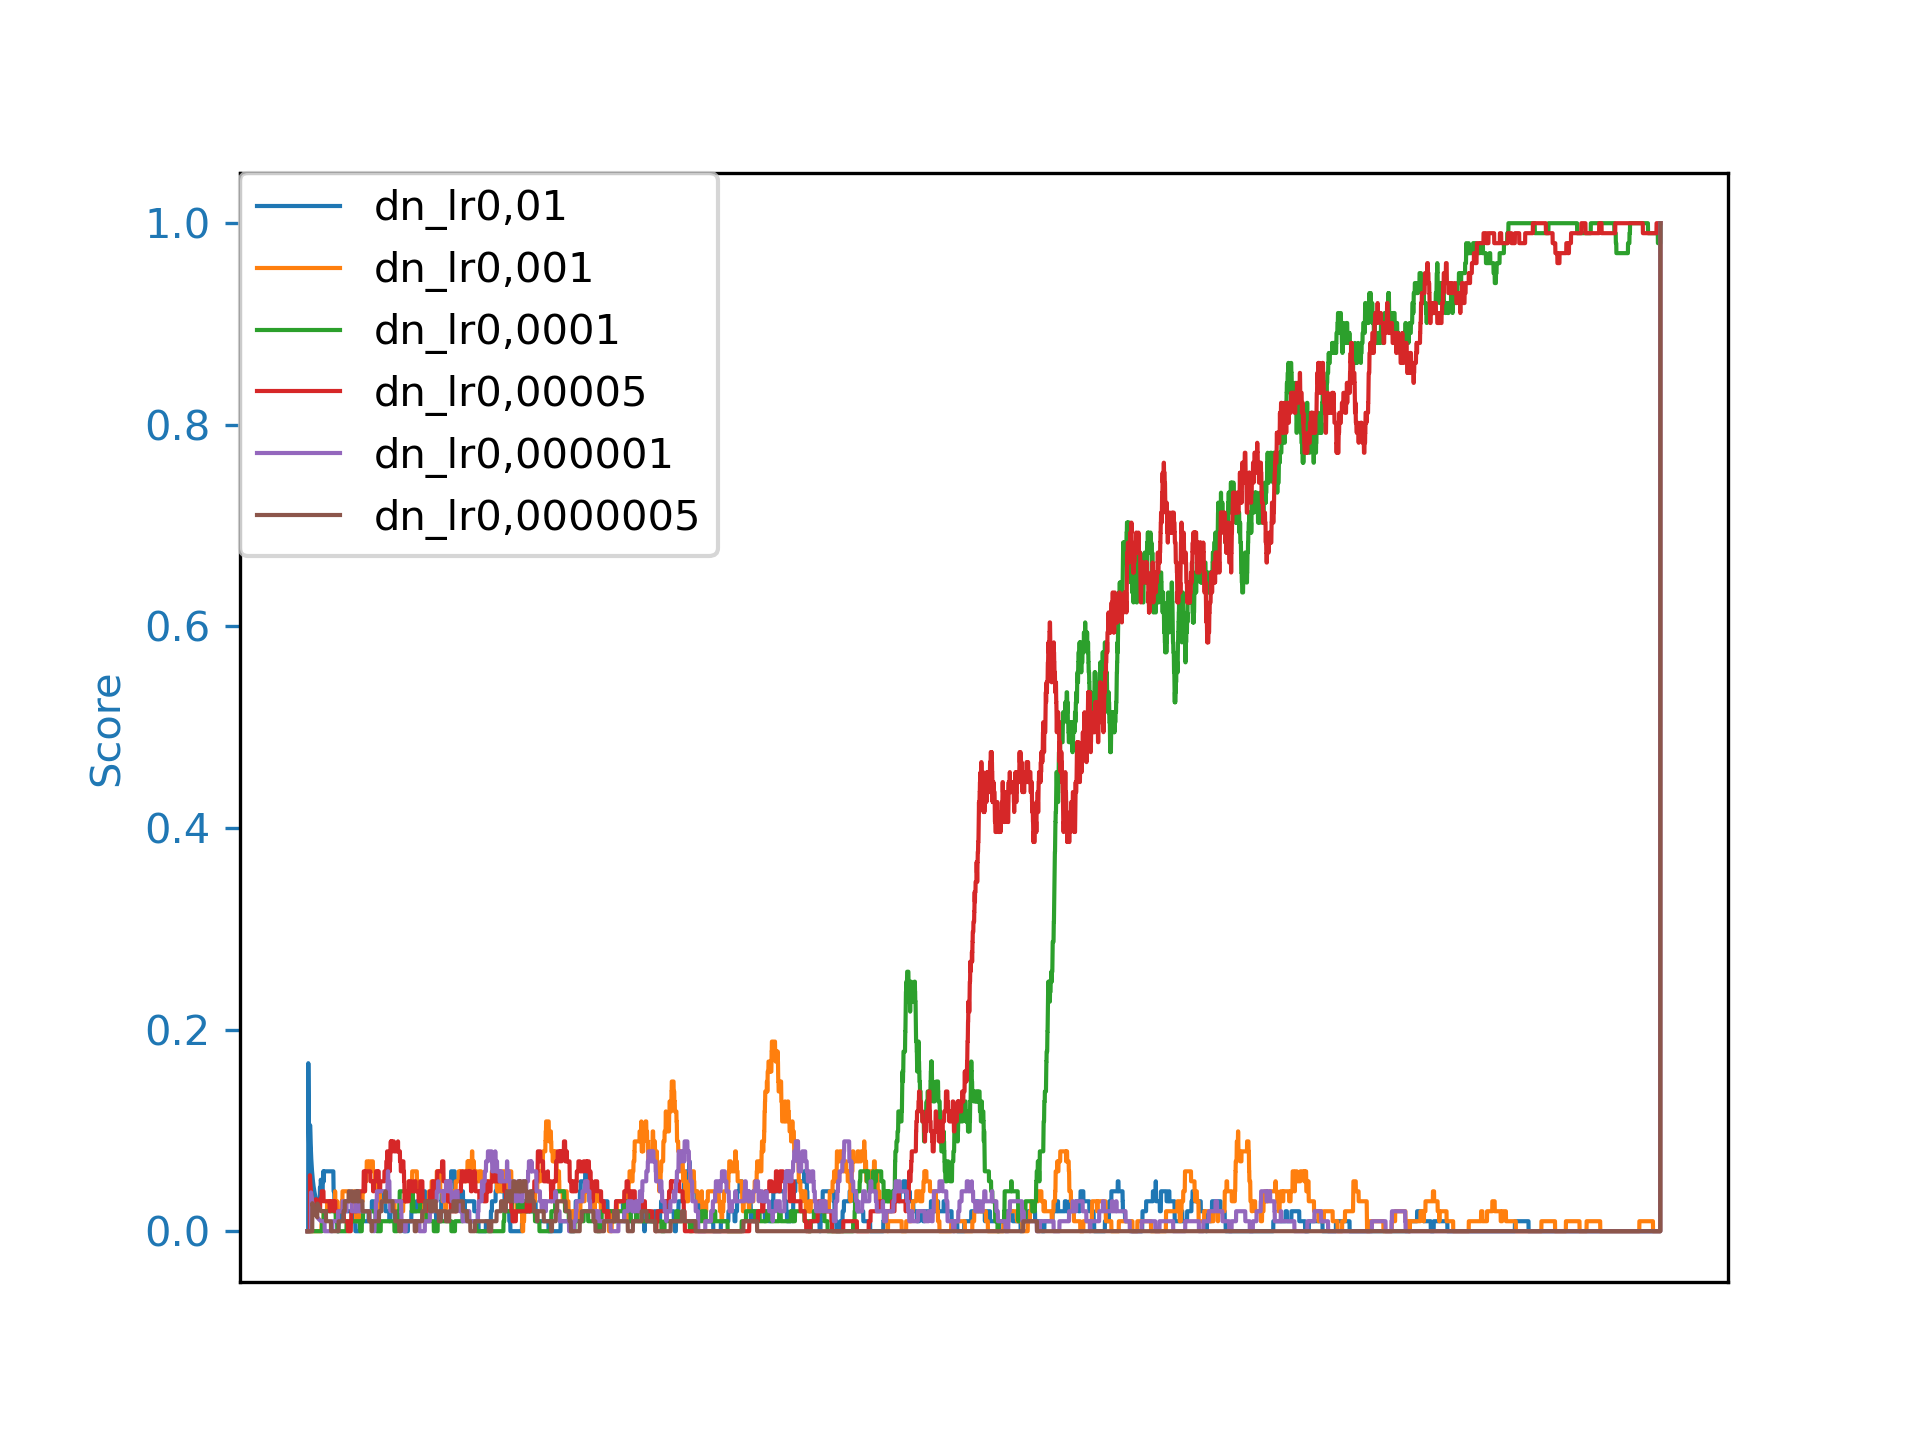
\includegraphics[width=\textwidth]{Figures/3x3_dn_lr0,01_dn_lr0,001_dn_lr0,0001_dn_lr0,00005_dn_lr0,000001_dn_lr0,0000005.png}
\caption{3x3 Neuronales Netz: Lernrate}
\label{dn4}
\end{figure}

Hier sieht man also, dass das Netz wirklich sehr empfindlich auf die Lernrate reagiert. Ein Wert von 0,00005 scheint in jedem Fall gut zu sein. Aber genau wie bei $\gamma$ kann man hier noch andere Werte in der Nähe testen.

Als letztes wollen wir das 4x4 Feld testen (Figure \ref{advanced1}). Dazu kombinieren wir verschiedene gute Parameter aus den vorigen Testläufen.

\begin{figure}[H]
\centering
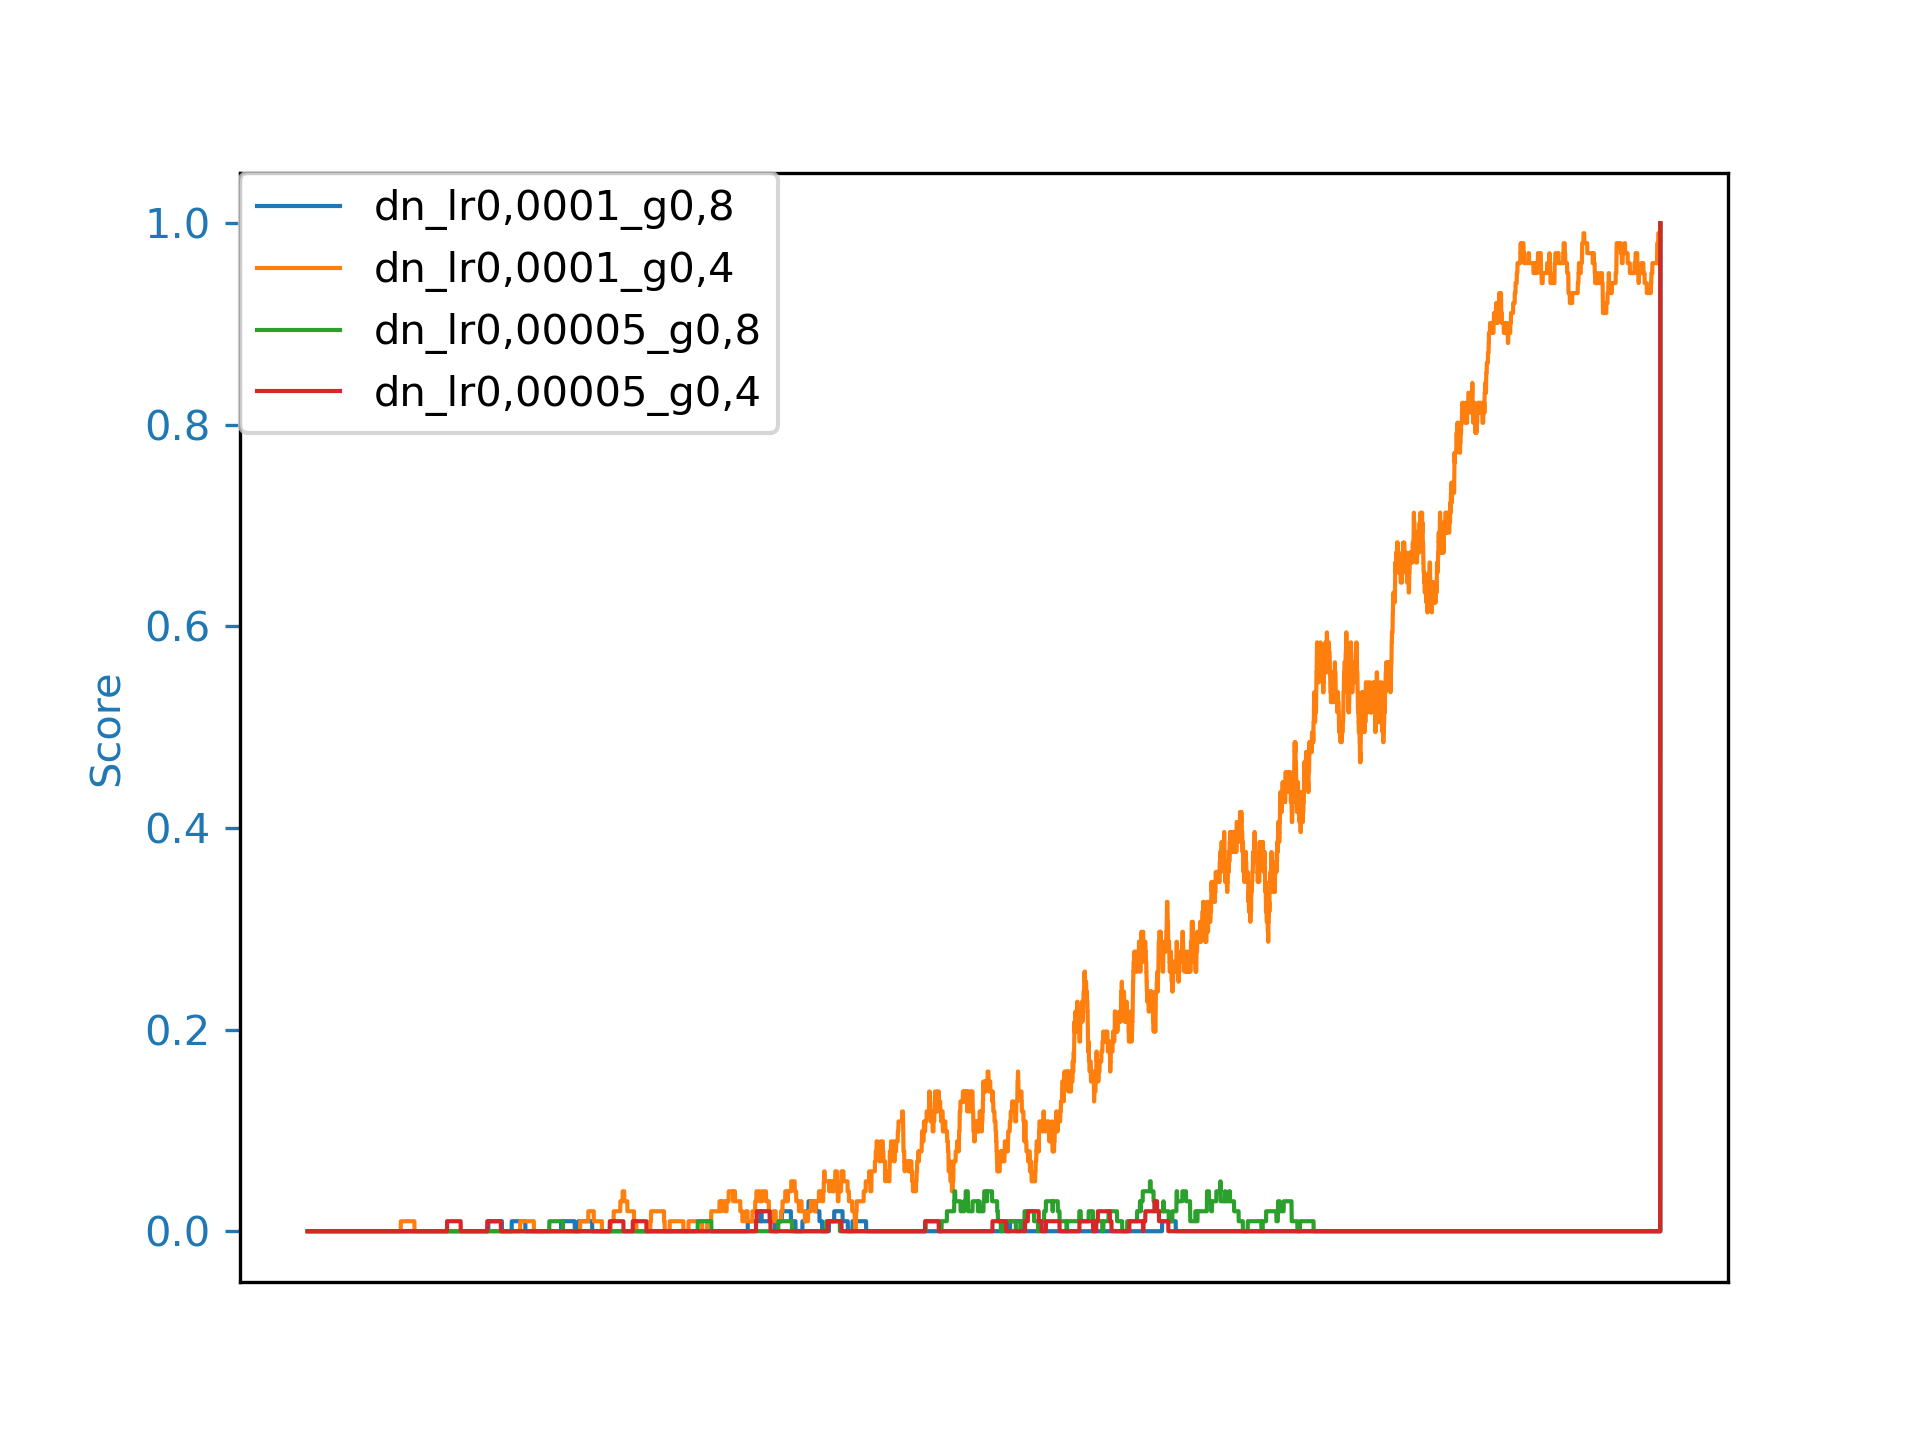
\includegraphics[width=\textwidth]{Figures/4x4_16_dn_lr0,0001_g0,8_dn_lr0,0001_g0,4_dn_lr0,00005_g0,8_dn_lr0,00005_g0,4.png}
\caption{4x4 Neuronales Netz: Gamma und Lernrate}
\label{dn5}
\end{figure}

Hier schneidet der Agent mit $\gamma$ = 0,4 und einer Lernrate von 0,0001 am besten ab. Meine erste Vermutung war hier, dass es sich um einen Zufall handelt und es davon abhängt, wie oft der Agent in den ersten 2000-3000 Spielen zufällig das Ziel findet. Durch eine Wiederholung des Experiments konnten wir das jedoch ausschließen. Mit anderen Parametern konnte zwar manchmal auch die beste Police gelernt werden, allerdings waren die gerade genannten Parameter immer am schnellsten.

\subsection{Beschränkte Boltzmann Maschine}
\label{subsec:dbm_r}

Bei der beschränkten Boltzmann Maschine haben wir 2 weitere Parameter. Zum einen den Wert $\beta$, der die Entropy abschwächt und zum anderen initialisieren wir die Gewichte am Anfang zufällig mit dem Erwartungswert 0 und einer Standardabweichung. Die Standardabweichung hat tatsächlich großen Einfluss auf das Ergebniss, da eine hohe Standardabweichung dazu führt, dass der Agent auf verschiedenen leeren Feldern sehr hohe Belohungen oder Bestrafungen erwartet. Diese Vorannahmen müssen dann erst wieder verlernt werden, was zu einem langsameren Lernverhalten führt.

Als erstes testen wir wieder, wie viele versteckte Neuronen wir brauchen:

\begin{figure}[H]
\centering
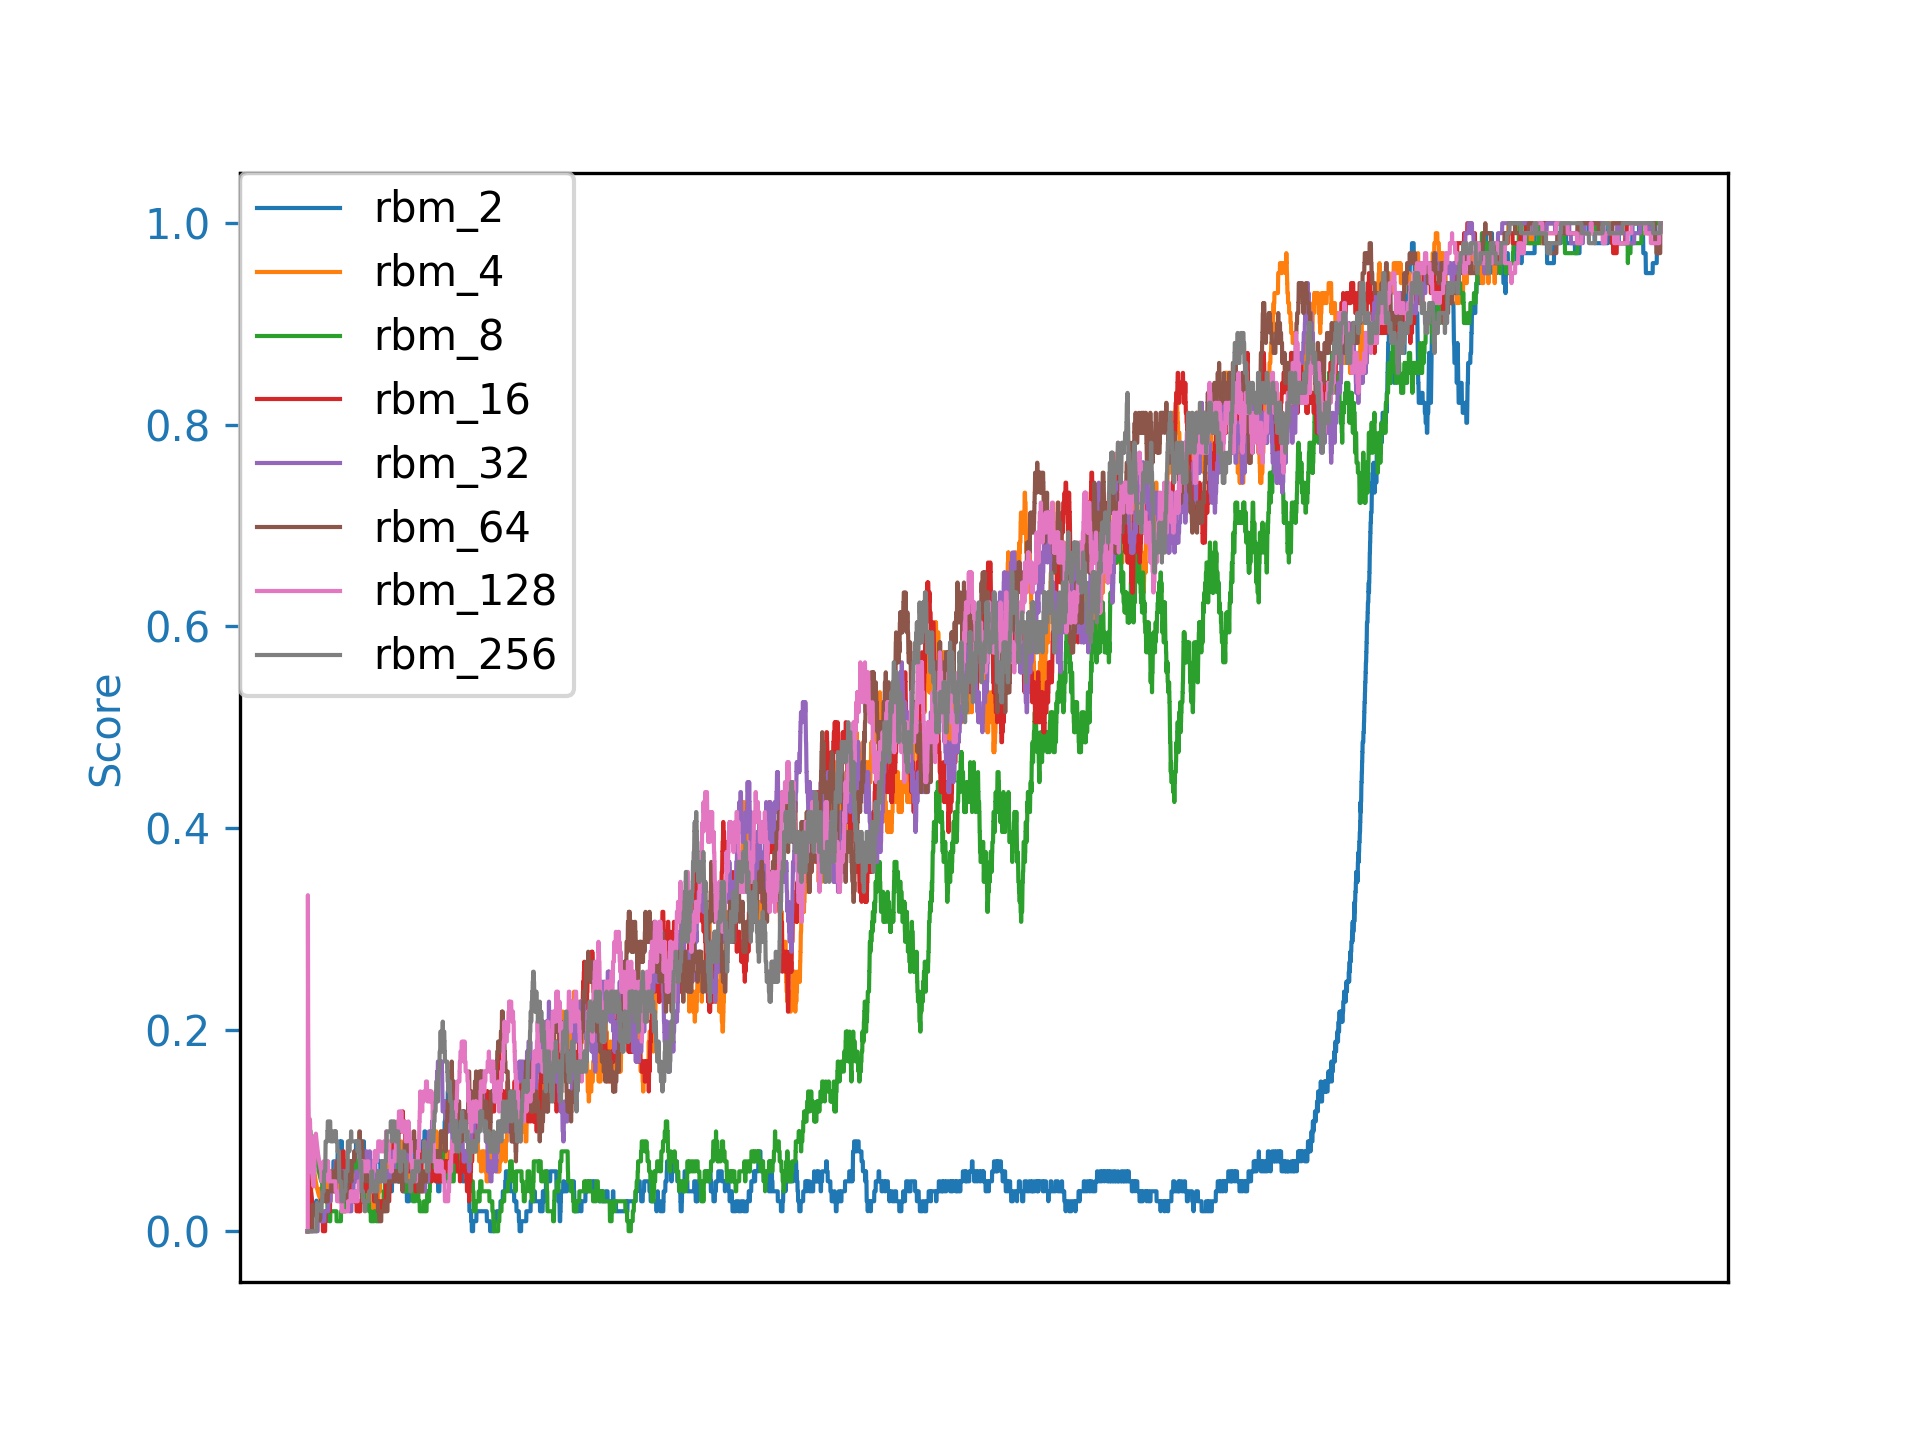
\includegraphics[width=\textwidth]{Figures/rbm6_3x3_rbm_2_rbm_4_rbm_8_rbm_16_rbm_32_rbm_64_rbm_128_rbm_256.png}
\caption{3x3 Beschränkte Boltzmann maschine: Neuronen}
\label{rbm1}
\end{figure}

Wir sehen hier also, je mehr Neuronen umso besser. Das ist schon ein erster spannender Unterschied zu dem einfachen neuronalen Netz, wo zu viele Neuronen schlecht waren. Allerdings führen viele Neuronen hier gleich zu einem deutlichen Anstieg an Rechenzeit. Daher wollen wir im Folgenden 16 Neuronen für das 3x3 Feld verwenden und nur bei größeren Feldern auf mehr Neuronen umsteigen.

Als nächstes wollen wir verschiedene Werte für $\gamma$ testen.

\begin{figure}[H]
\centering
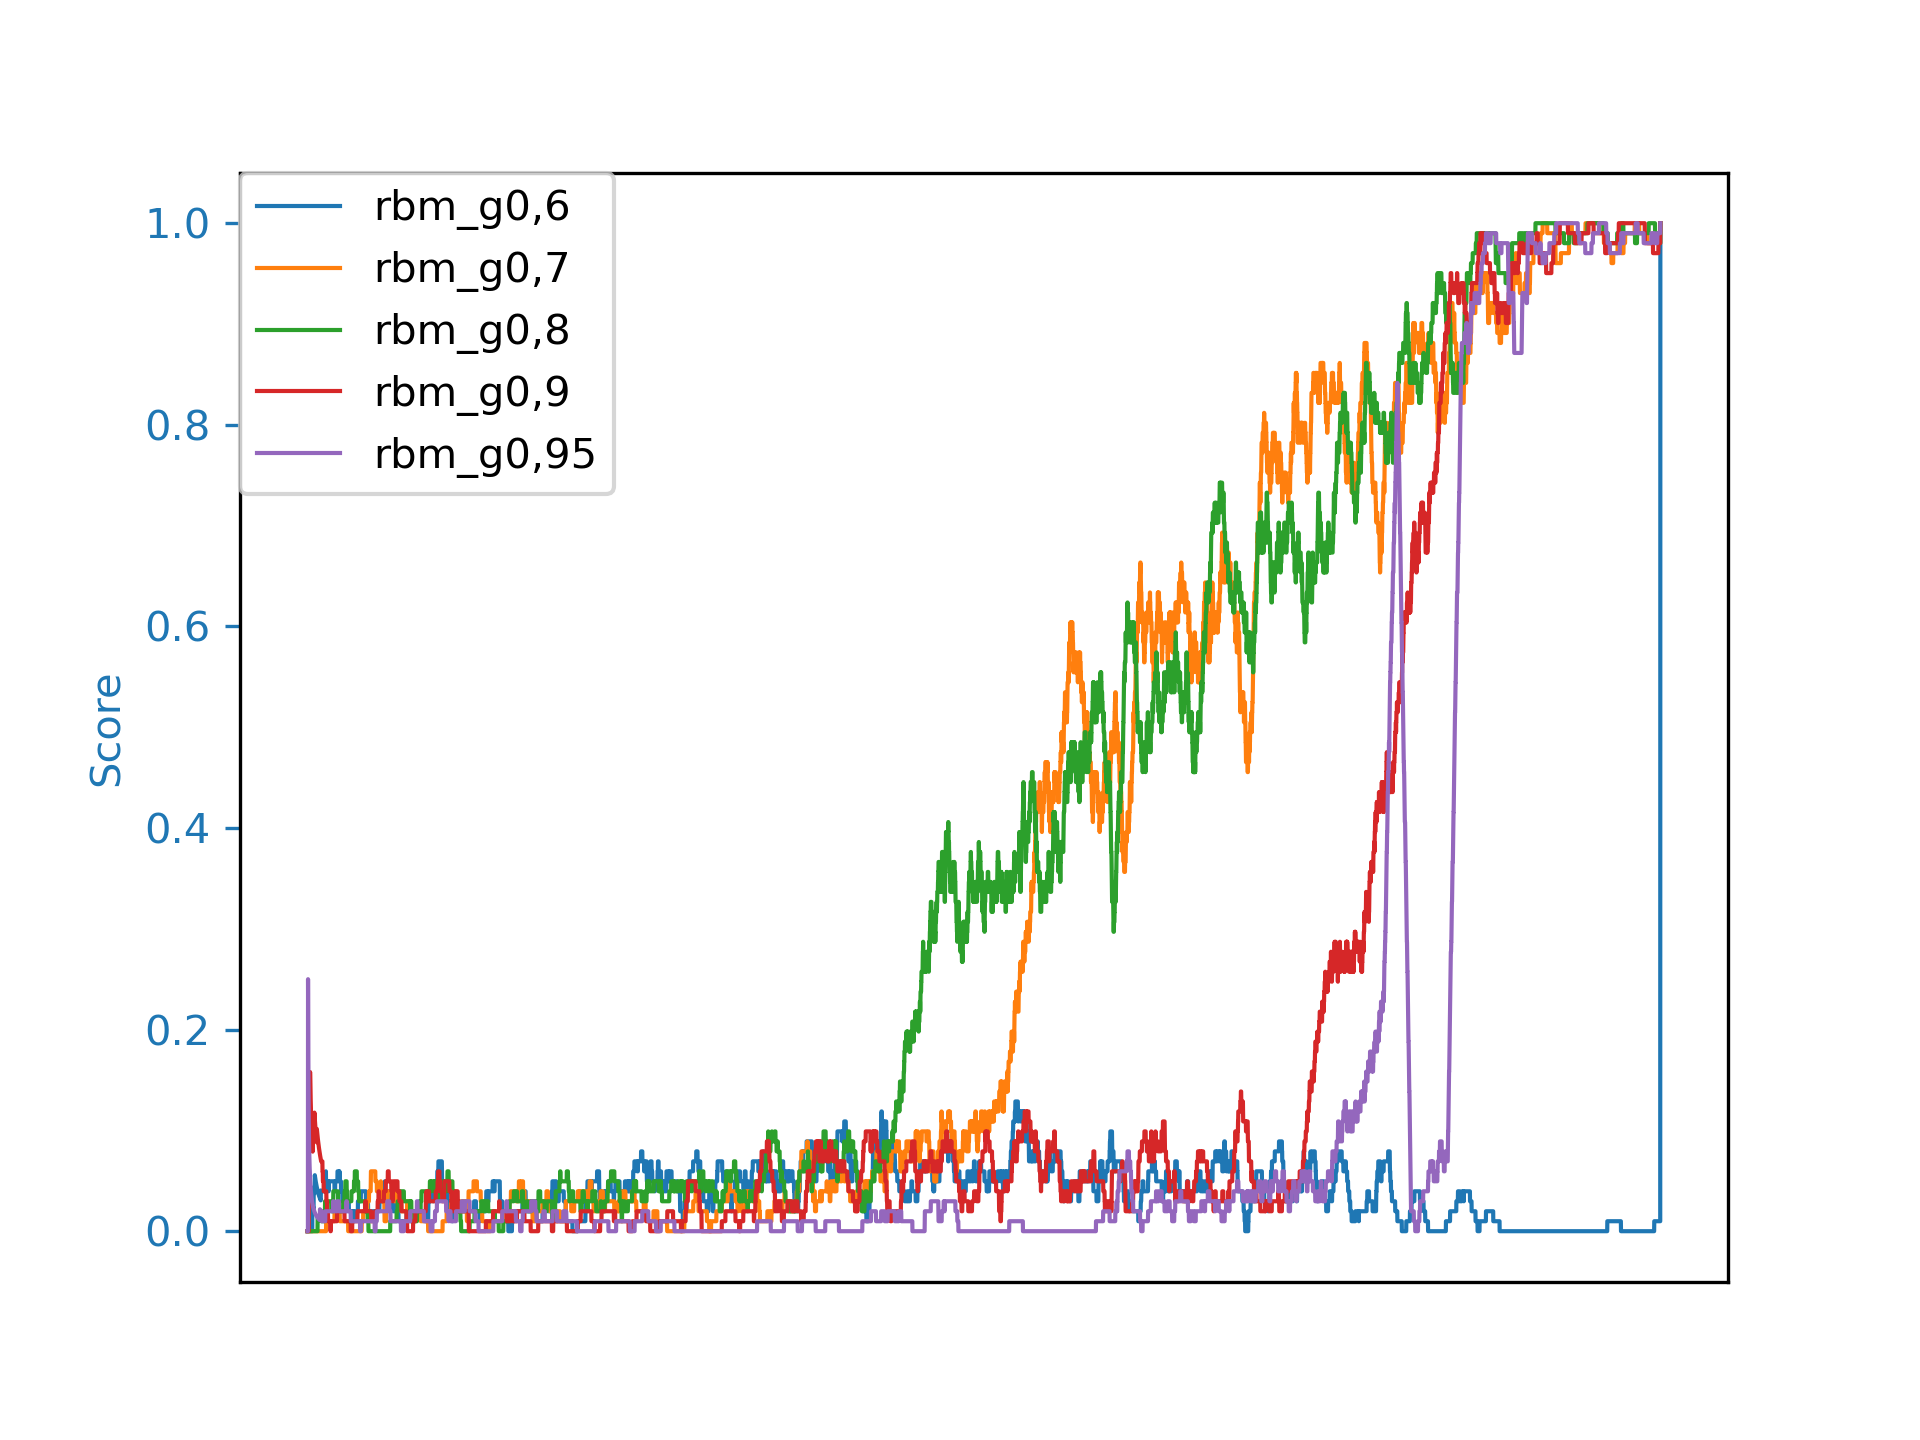
\includegraphics[width=\textwidth]{Figures/rbm3_3x3_rbm_g0,6_rbm_g0,7_rbm_g0,8_rbm_g0,9_rbm_g0,95.png}
\caption{3x3 Beschränkte Boltzmann maschine: $\gamma$}
\label{rbm2}
\end{figure}

Die besten Ergebnisse bekommen wir also mit einem $\gamma$- Wert von 0,7 oder 0,8. Daher bleiben wir im weiteren wie in \citep{crawford2019reinforcement} bei 0,8.

Wir wollen nun $\beta$ vergleichen. Mit $\beta$ schwächen wir die zweite Summe in (\ref{F}) ab. Dadurch können wir steuern, wie stark die Werte der versteckten Neuronen richtung 0 oder 1 gesteuert werden.

\begin{figure}[H]
\centering
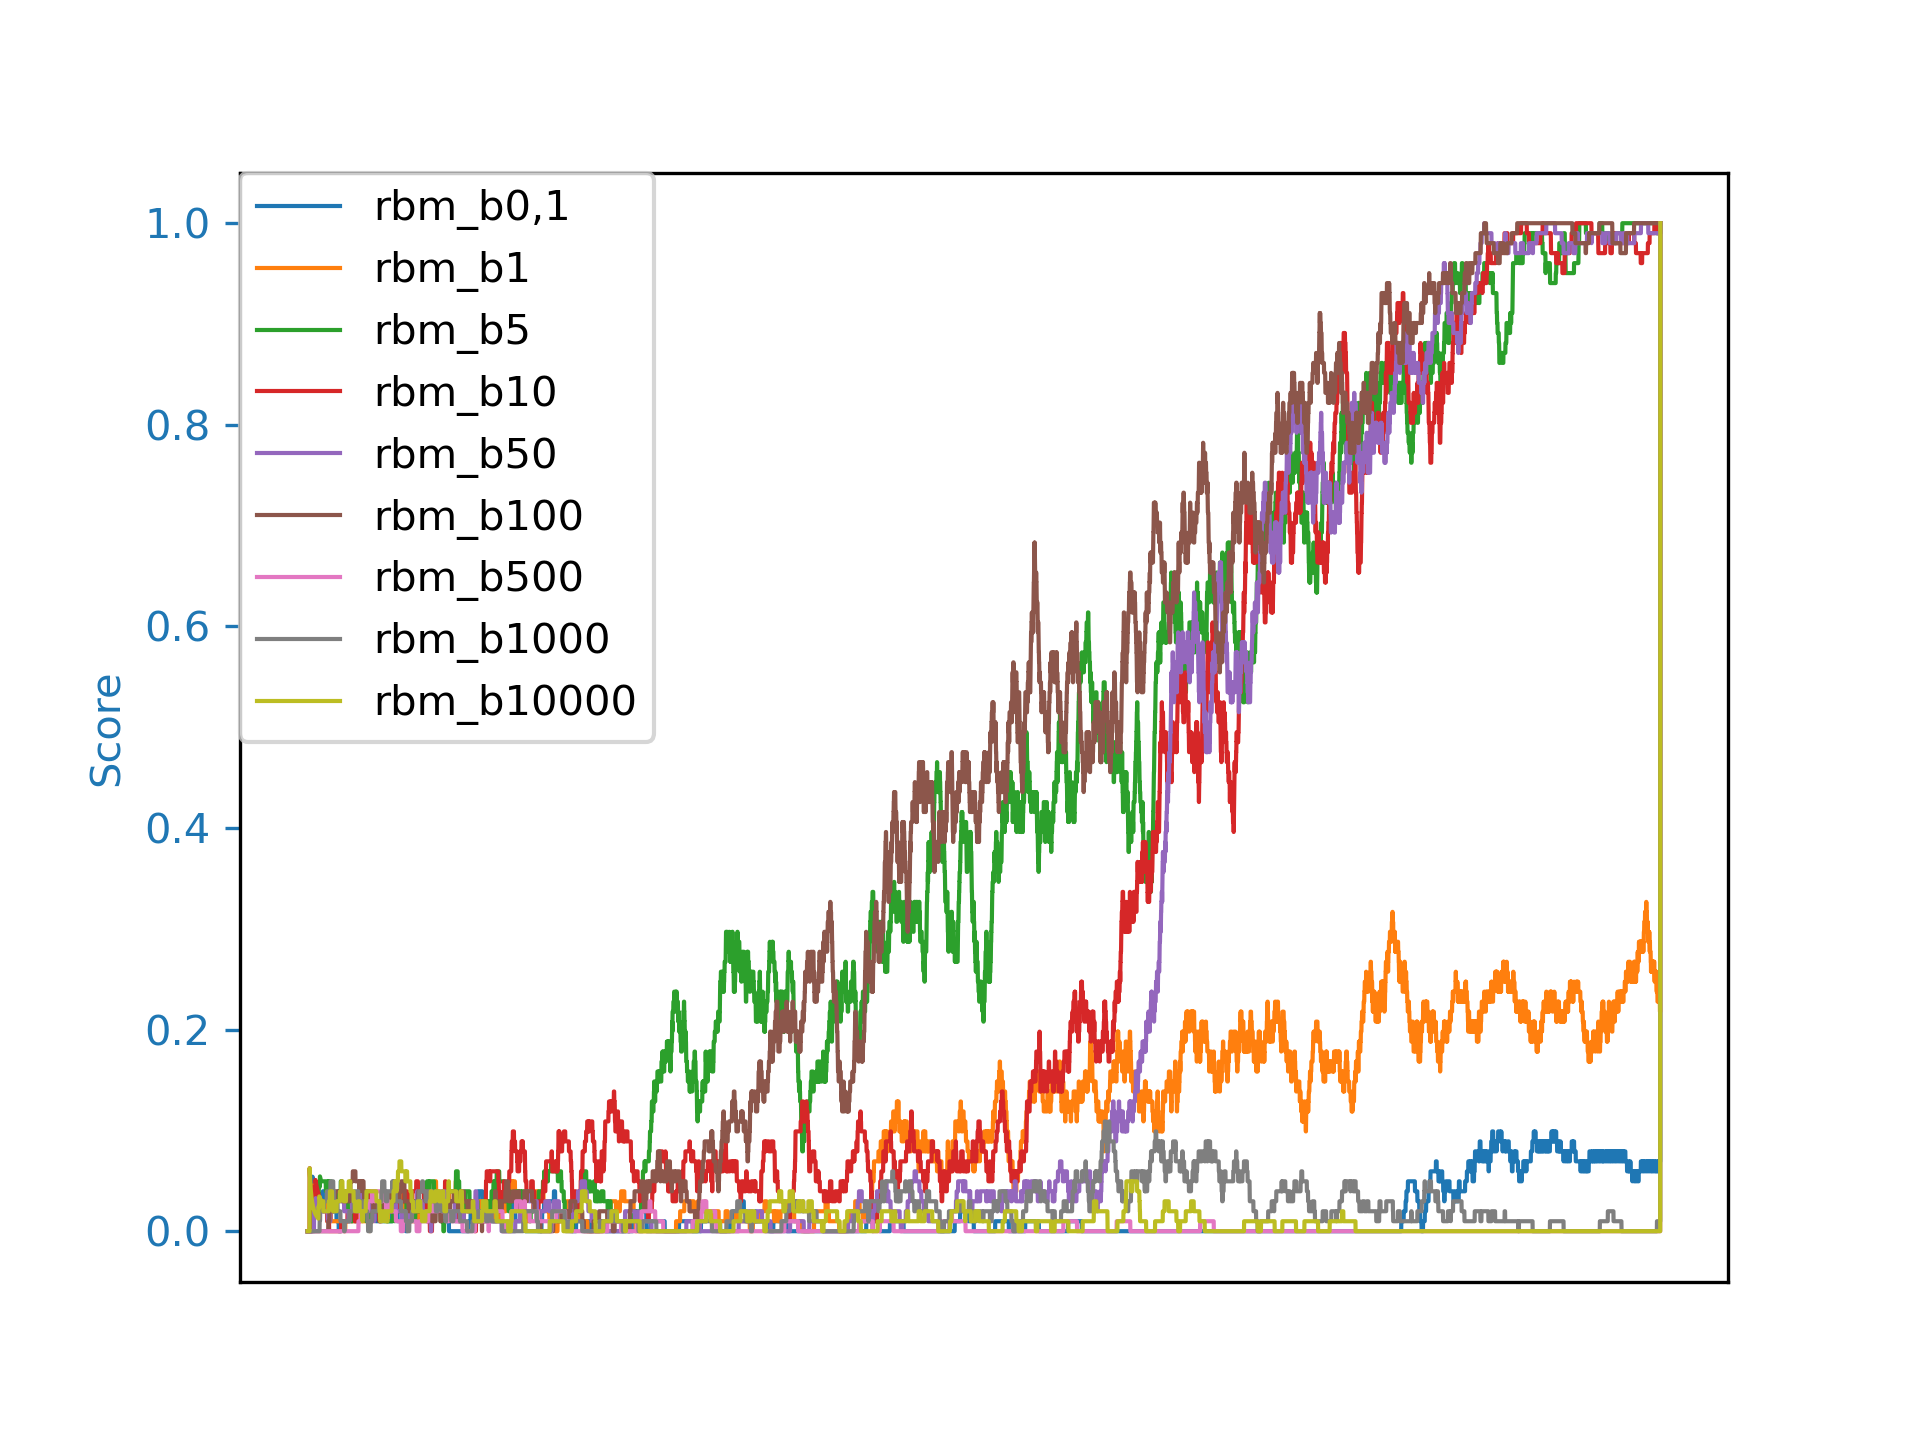
\includegraphics[width=\textwidth]{Figures/rbm4_3x3_rbm_b0,1_rbm_b1_rbm_b5_rbm_b10_rbm_b50_rbm_b100_rbm_b500_rbm_b1000_rbm_b10000.png}
\caption{3x3 Beschränkte Boltzmann maschine: $\beta$}
\label{rbm3}
\end{figure}

Wir sehen hier, dass bei Werten zwischen 5 und 100 richtige Policen gefunden werden. Es scheint also sinnvoll zu sein, diesen Entropy-Faktor stark abzuschwächen. aber nicht ganz wegzulassen. Wir verwenden im Folgenden einen mittleren Wert von 20.

Nun schauen wir uns die Lernrate an:

\begin{figure}[H]
\centering
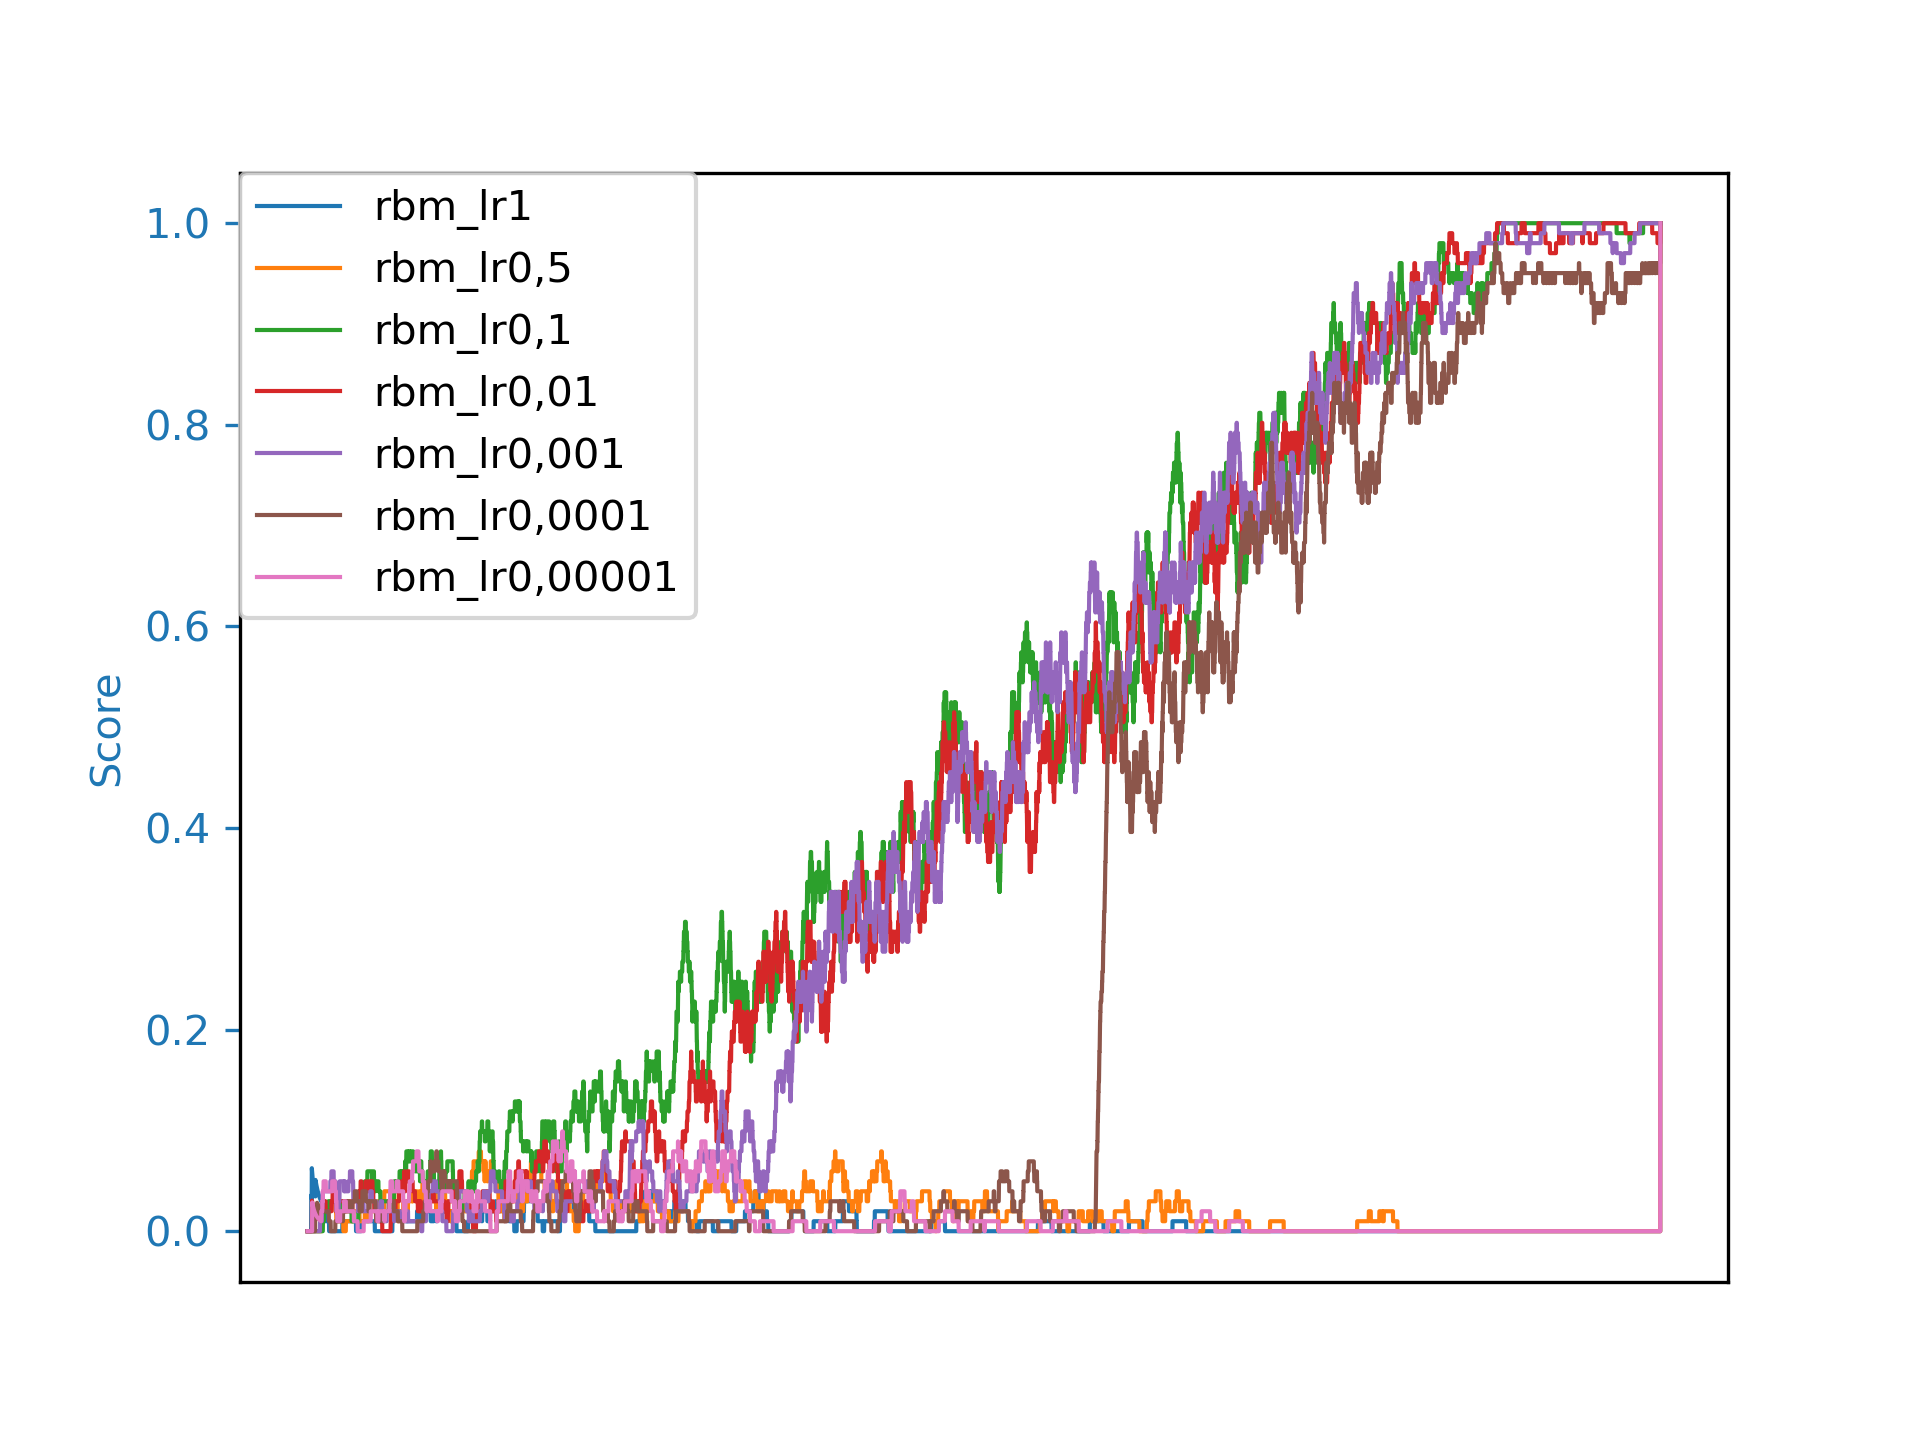
\includegraphics[width=\textwidth]{Figures/rbm5_3x3_rbm_lr1_rbm_lr0,5_rbm_lr0,1_rbm_lr0,01_rbm_lr0,001_rbm_lr0,0001_rbm_lr0,00001.png}
\caption{3x3 Beschränkte Boltzmann maschine: Lernrate}
\label{rbm4}
\end{figure}

Hier sehen wir gute Ergebnisse zwischen 0,1 und 0,001. Daher nehmen wir auch hier den mittleren Wert von 0,01 für folgende Experimente.

Als letztes testen wir die Standardabweichung für die Initialisierung der Gewichte.

\begin{figure}[H]
\centering
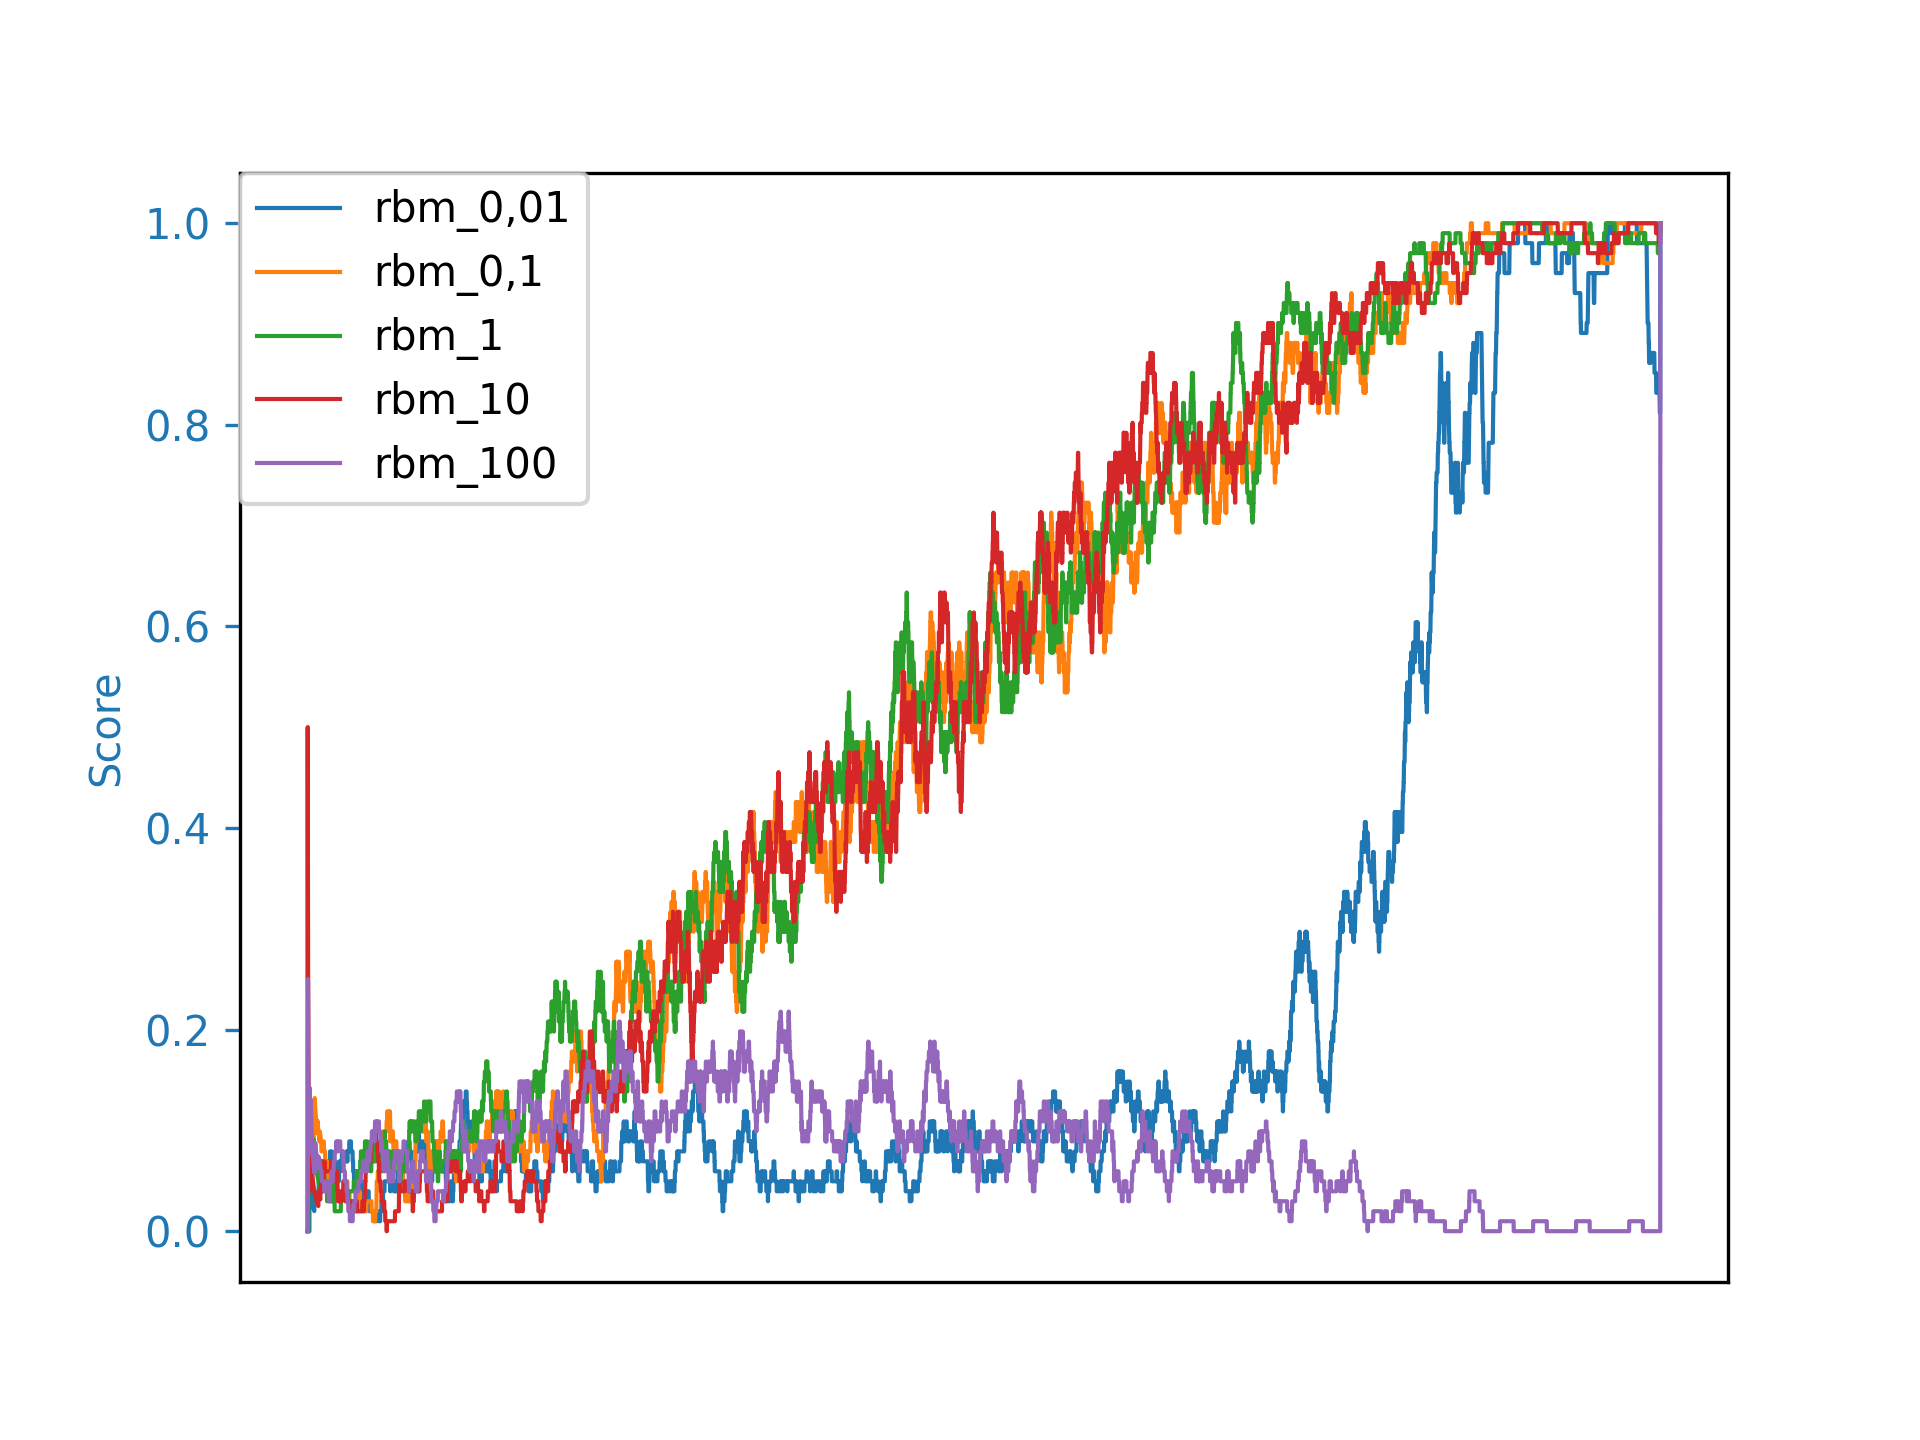
\includegraphics[width=\textwidth]{Figures/rbm7_3x3_rbm_0,01_rbm_0,1_rbm_1_rbm_10_rbm_100.png}
\caption{3x3 Beschränkte Boltzmann maschine: Standardabweichung}
\label{rbm5}
\end{figure}

Wir sehen also, dass zu große oder zu kleine Werte zu schlechteren Ergebnissen führen und verwenden genau wie in \citep{crawford2019reinforcement} die übliche Standardabweichung von 1.

Da wir bei den Feldern aus (Figure \ref{advanced1}) und (Figure \ref{advanced2}) noch sehr gute Ergebnisse bekommen und sogar verschiedene Parameter alle zuverlässig das richtige Ergebnis liefern, wollen wir hier gleich zu dem 5x5 Spielfeld übergehen. Hier testen wir sowohl mit 16 als auch mit 64 Neuronen und mit $\beta$ von 10 und 50:

\begin{figure}[H]
\centering
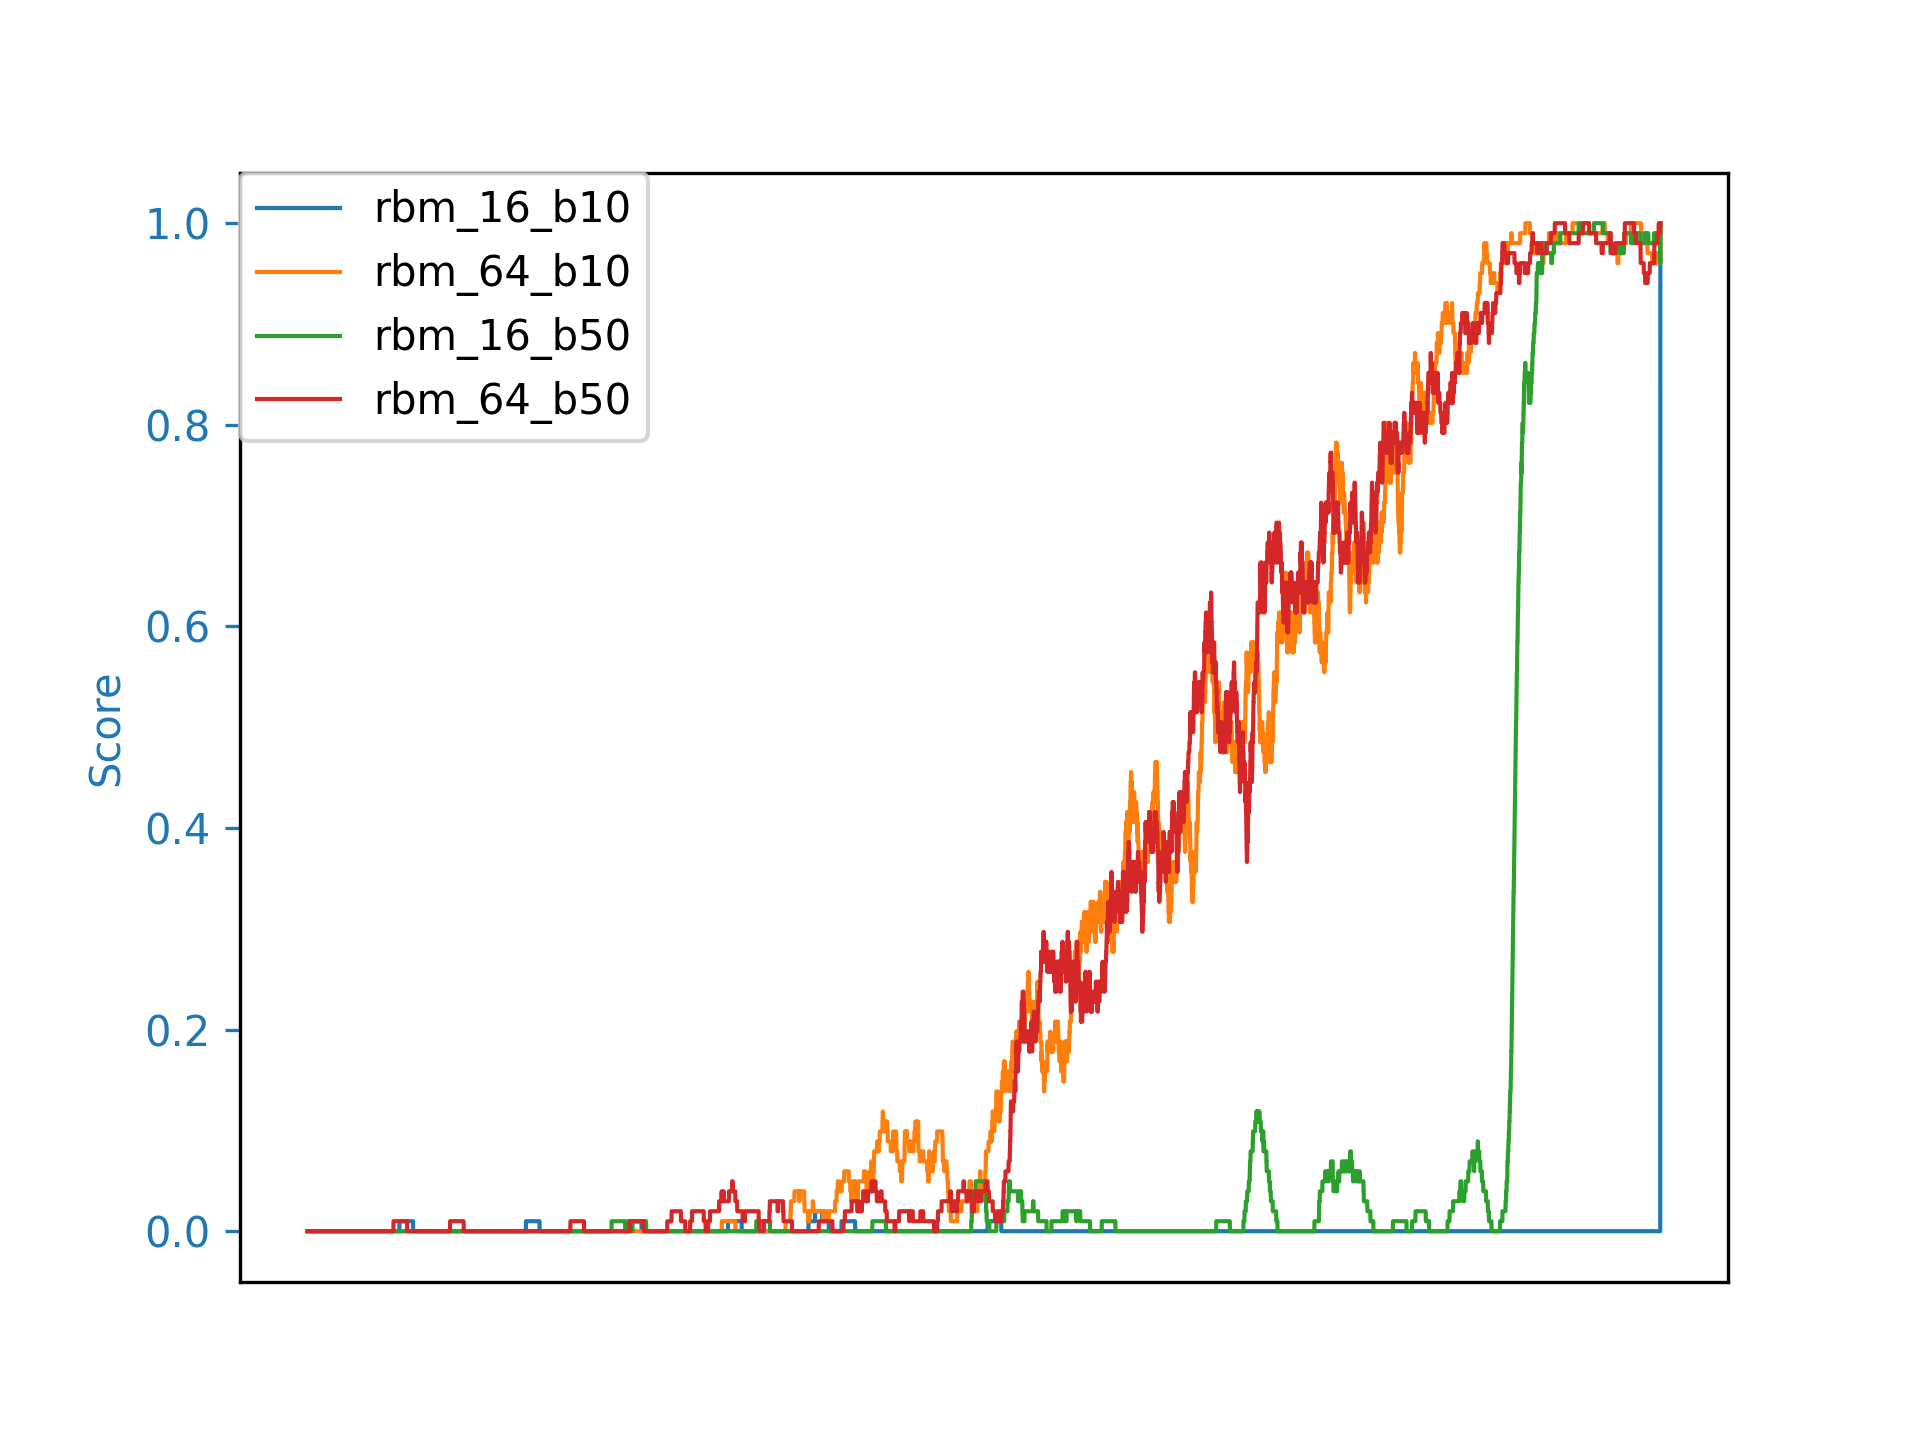
\includegraphics[width=\textwidth]{Figures/rbm8_5x5_rbm_16_b10_rbm_64_b10_rbm_16_b50_rbm_64_b50.png}
\caption{5x5 Beschränkte Boltzmann maschine: Neuronen und $\beta$}
\label{rbm5}
\end{figure}

Hier sehen wir zum ersten Mal, wie 16 Neuronen nicht mehr ausreichen. Der $\beta$-Wert dageben scheint in einer recht großen Spannweite gut zu funktionieren. Wobei anscheinend der Wert 50 sogar besser ist, da hier selbst mit 16 Neuronen noch die richtige Police gefunden wurde.

\subsection{Tiefe Boltzmann Maschine Resultate mit Quanten Annealing}
\label{subsec:dbm_r}

Die Neuheit bei diesem Algorithmus ist vor allem, dass wir die Aktivierung der versteckten Neuronen mit simuliertem Quanten Annealing berechnen. Daher kommen hier 3 neue Parameter hinzu: Anzahl der Annealing-Durchläufe, Anzahl der Schritte beim Annealing und die Annealing Temperatur, die aus einem Startwert und einem Endwert besteht. 

Die Anzahl der Annealing-Durchläufe und die Anzahl der Schritte beim Annealing sollten möglichst hoch gewählt werden, da wir so genauere Ergebnisse bekommen. Gleichzeitig sind diese beiden Parameter für einen starken Anstieg der Rechenzeit verantwortlich. Daher setzen wir beide für unsere Testdurchläufe für die anderen Parameter auf 100. So bekommen wir auch noch in akzeptabler Zeit Ergebnisse. Später für die Vergleiche zwischen den verschiedenen Algorithmen können wir noch höhere Werte nehmen. Um diese beiden Werte zu testen, kann man 100 mal die Aktivierung der versteckten Neuronen berechnen und aus diesen 100 Vektoren die Standardabweichung berechnen. Diese liegt zwischen 0.01 und 0.03 mit den gerade genannten Parametern.

Die Annealing Temperatur sollte so gewählt werden, dass wir gute Ergebnisse bekommen, aber nicht immer das Richtige. Wenn wir immer das bestmögliche Ergebniss berechnen würden,  wären unsere versteckten Neuronen immer 1 oder 0 und damit hätten wir keine sauberen Übergänge zwischen den Lernphasen sondern ``Brüche'' wenn die versteckten Neuronen den Zustand wechseln. Dies führt zu schlechteren Ergebnissen. Wir starten hier mit dem Startwert 2 und dem Endwert 20, wie auch in \citep{crawford2019reinforcement}.

Dafür können wir in diesem Verfahren $\beta$ weglassen, da wir die Entropy über die Annealing Temperatur steuern können. Konkreter gesagt, wenn wir die Temperatur sehr gut wählen, bekommen wir immer das optimale Ergebniss und das wiederum führt zu einer maximalen Entropy. Diese Vermutung werden wir später noch mit Tests bestätigen.

Starten wir unsere Tests mit der Anzahl an Neuronen:

\begin{figure}[H]
\centering
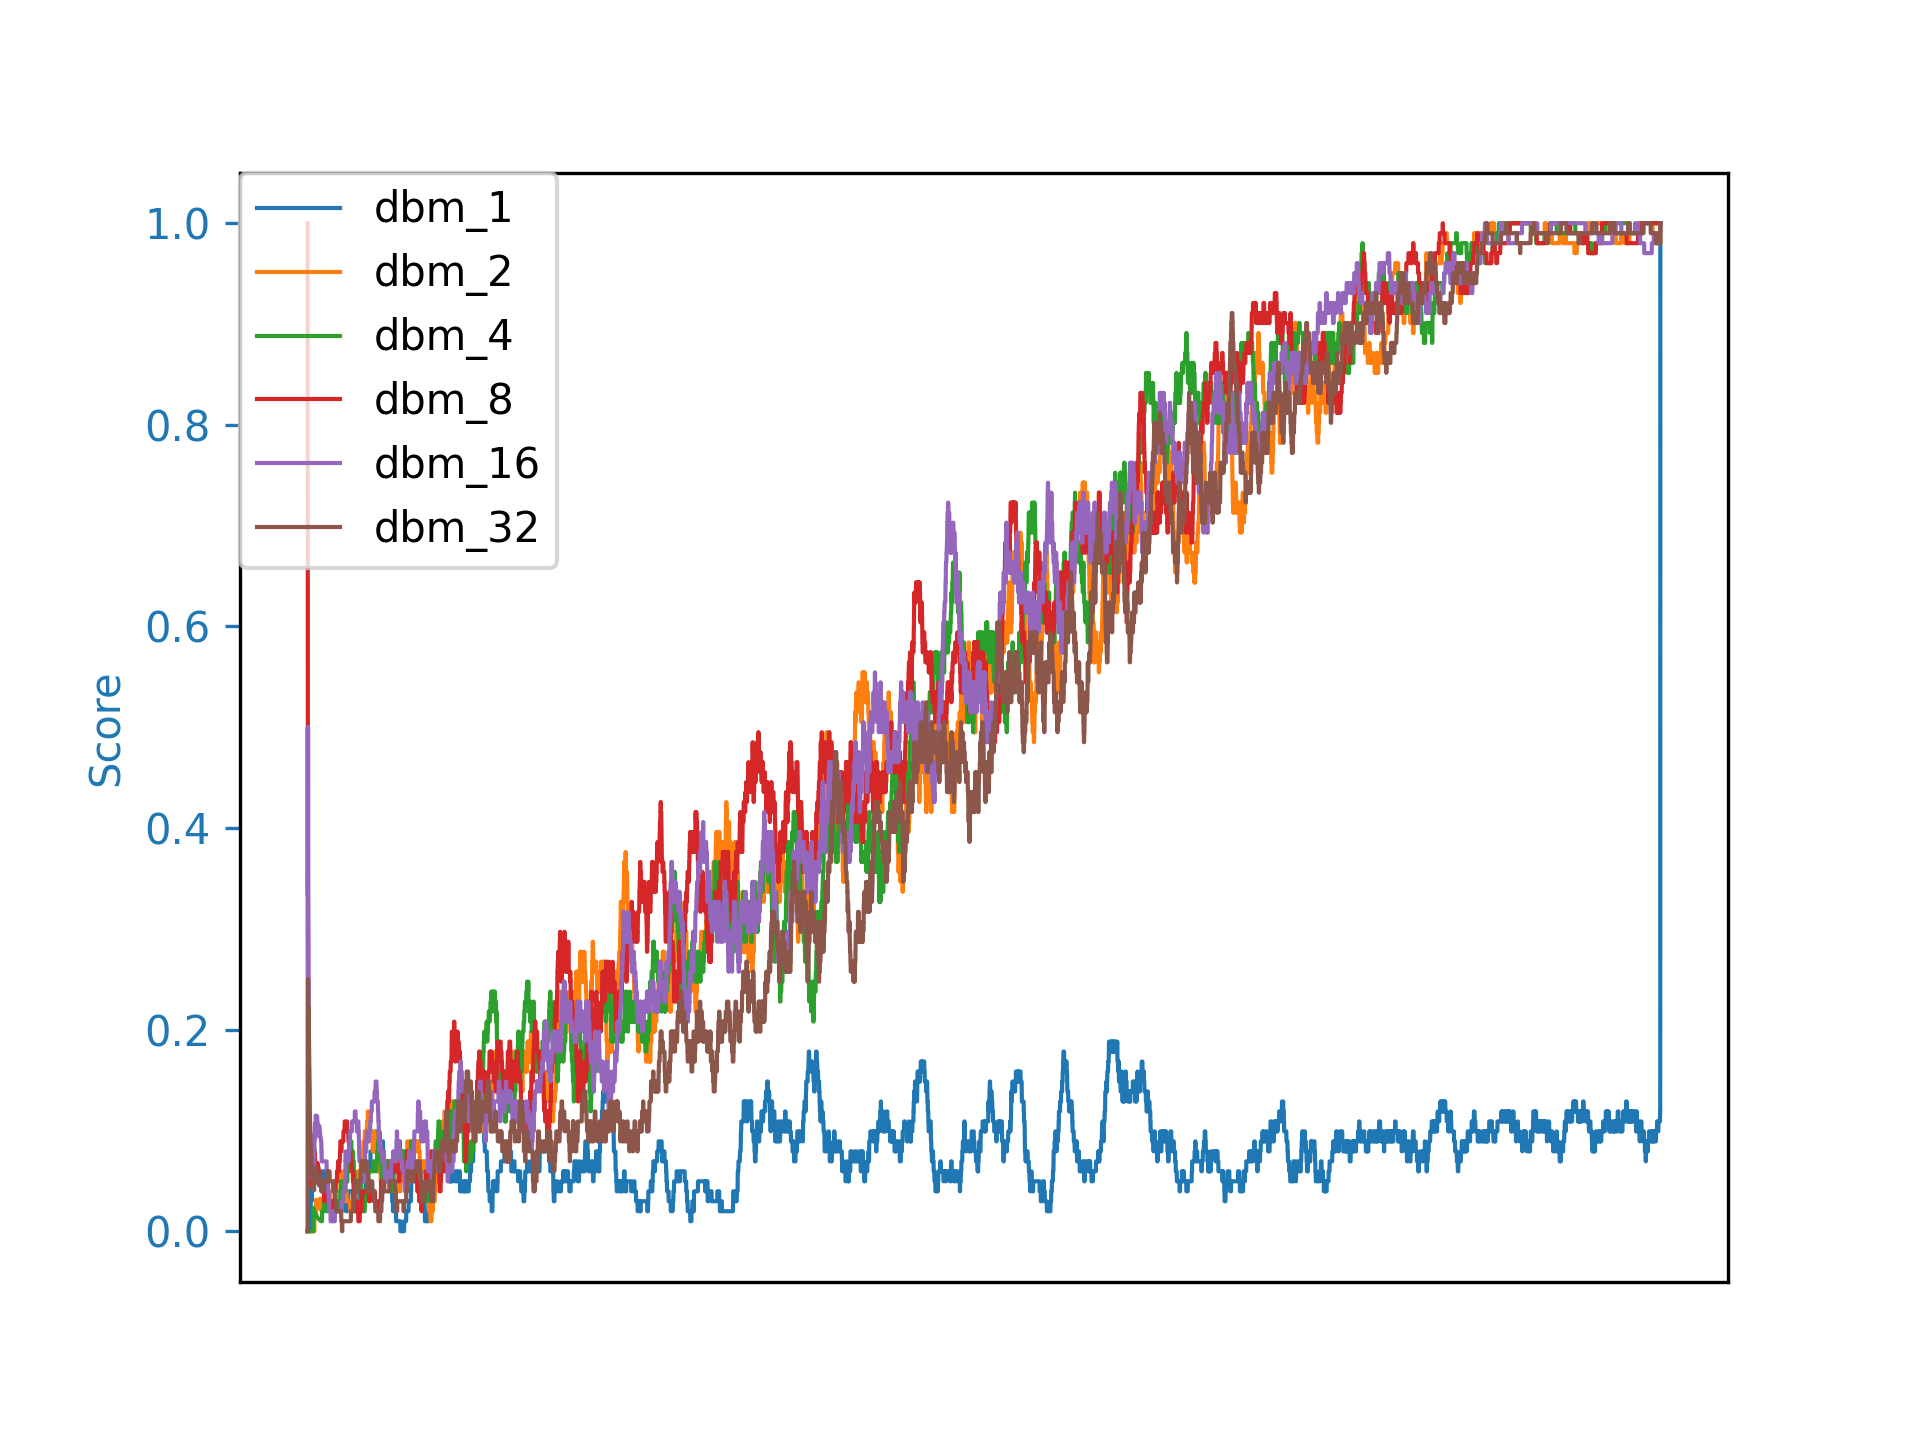
\includegraphics[width=\textwidth]{Figures/dbm1_3x3_dbm_1_dbm_2_dbm_4_dbm_8_dbm_16_dbm_32.png}
\caption{3x3 Tiefe Boltzmann maschine: Neuronen}
\label{dbm1}
\end{figure}

Hier zeigt sich bereits die Stärke dieses Verfahrens. Während wir beim einfachen neuronalen Netz mindestens 8 Neuronen gebraucht haben, brauchen wir hier nur 2. Die beschränkte Boltzmann Maschine konnte dieses Beispiel zwar auch mit 2 Neuronen lösen, fand die richtige Police allerdings sehr spät. Nach oben scheint es hier keine Grenze zu geben, obwohl die Version mit 32 Neuronen minimal langsamer reagiert. Eine höhere Anzahl von Neuronen führt hier bereits zu sehr langen Rechenzeiten, weswegen wir diese hier nicht testen.

Als nächstes schauen wir uns wieder $\gamma$ an. Da die Ergebnisse hier nur für extreme Randwerte schlechter werden, testen wir es auch gleich noch auf dem 4x4 Spielfeld:

\begin{figure}[H]
\centering
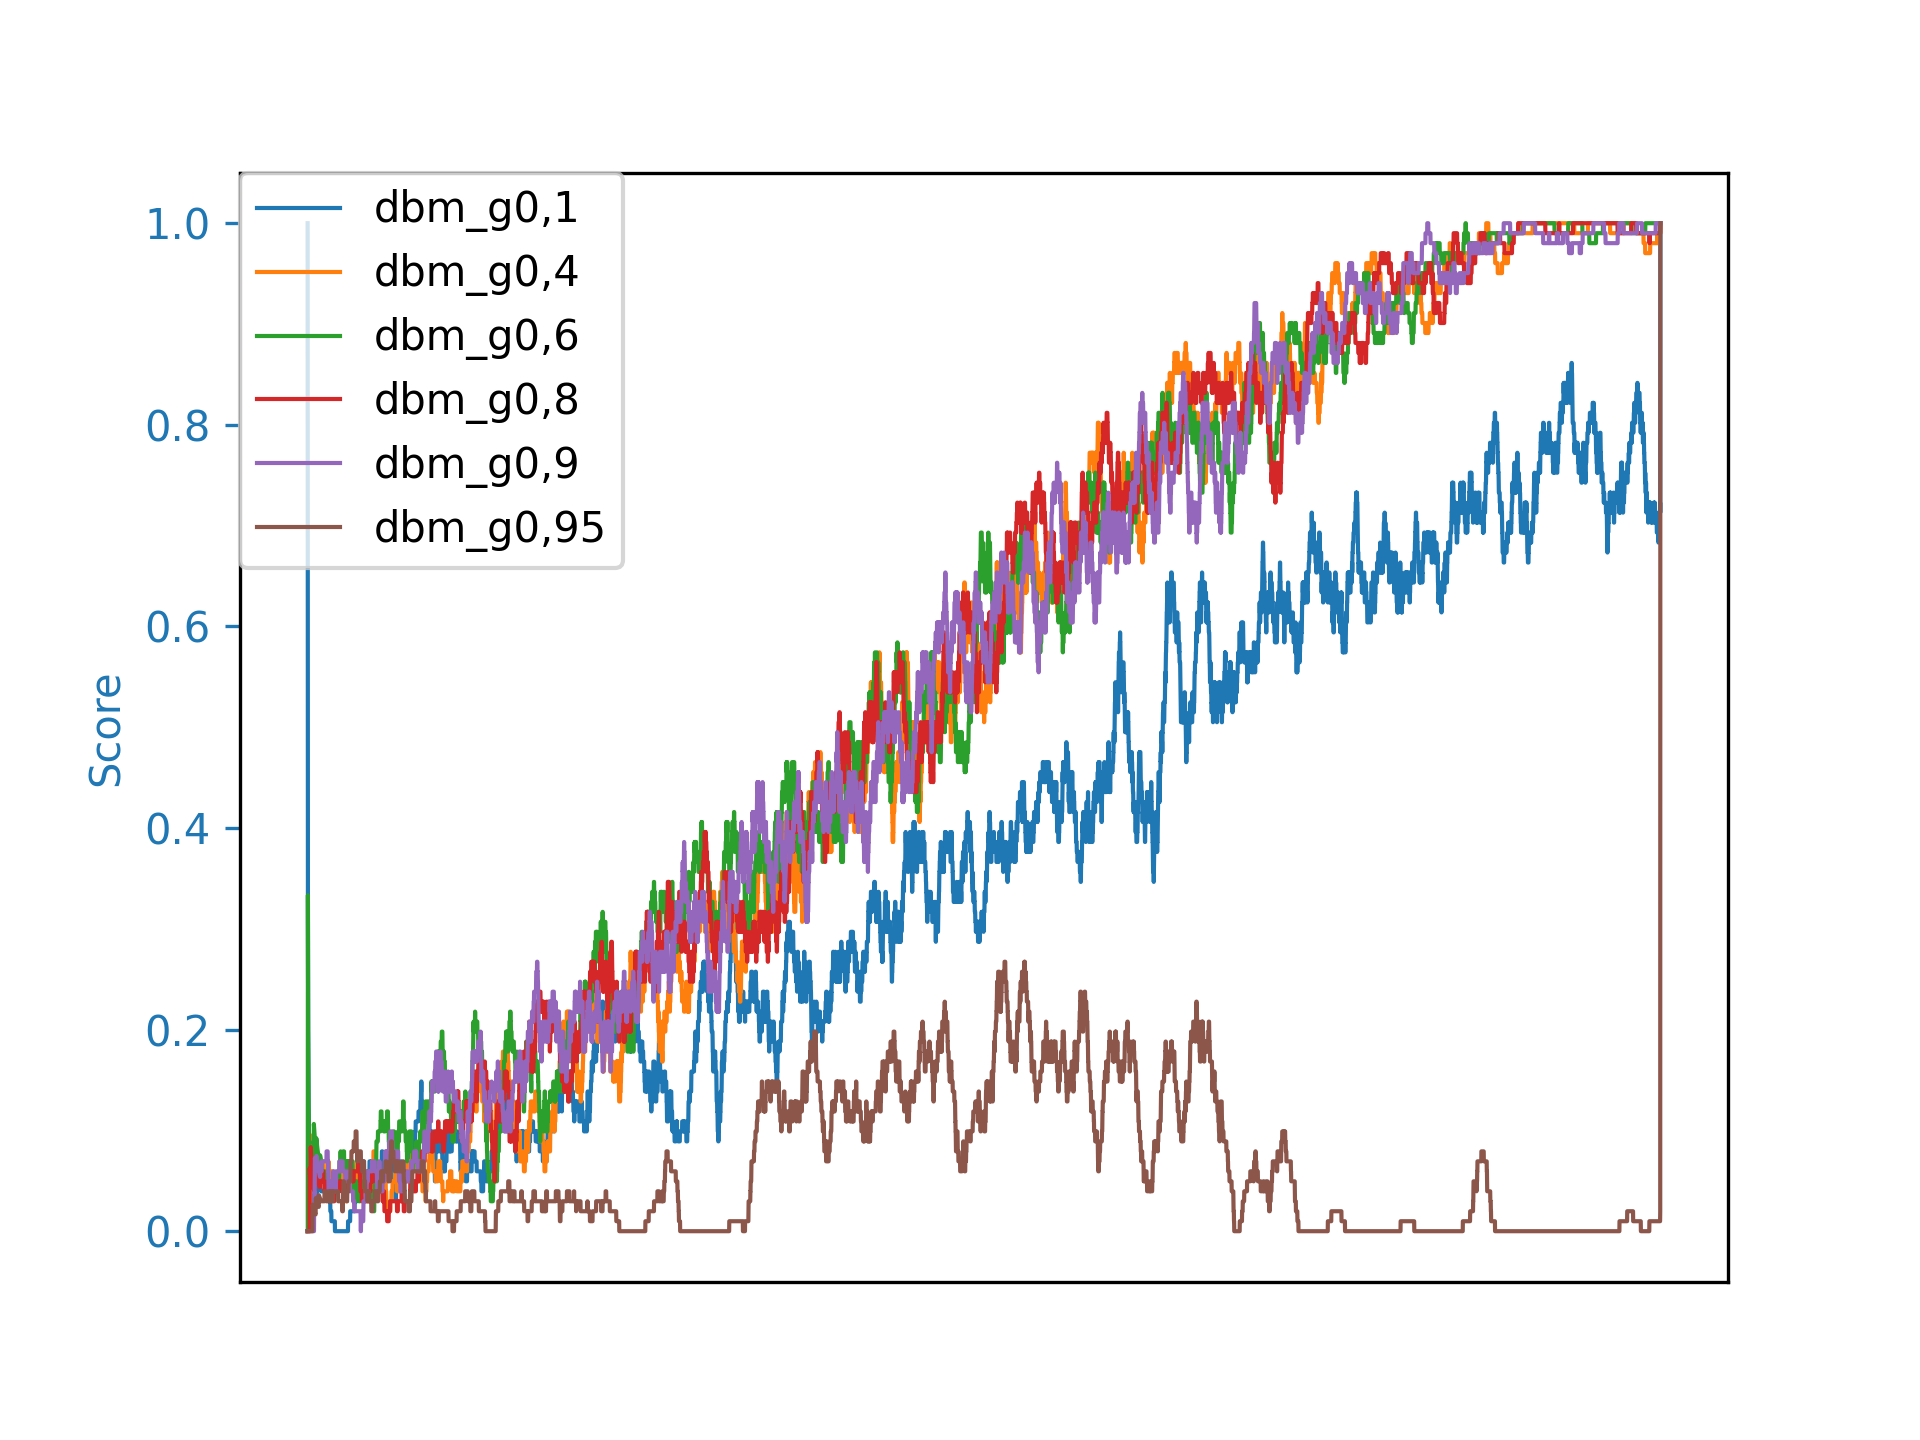
\includegraphics[width=\textwidth]{Figures/dbm4_3x3_dbm_g0,1_dbm_g0,4_dbm_g0,6_dbm_g0,8_dbm_g0,9_dbm_g0,95.png}
\caption{3x3 Tiefe Boltzmann maschine:$\gamma$}
\label{dbm1}
\end{figure}

\begin{figure}[H]
\centering
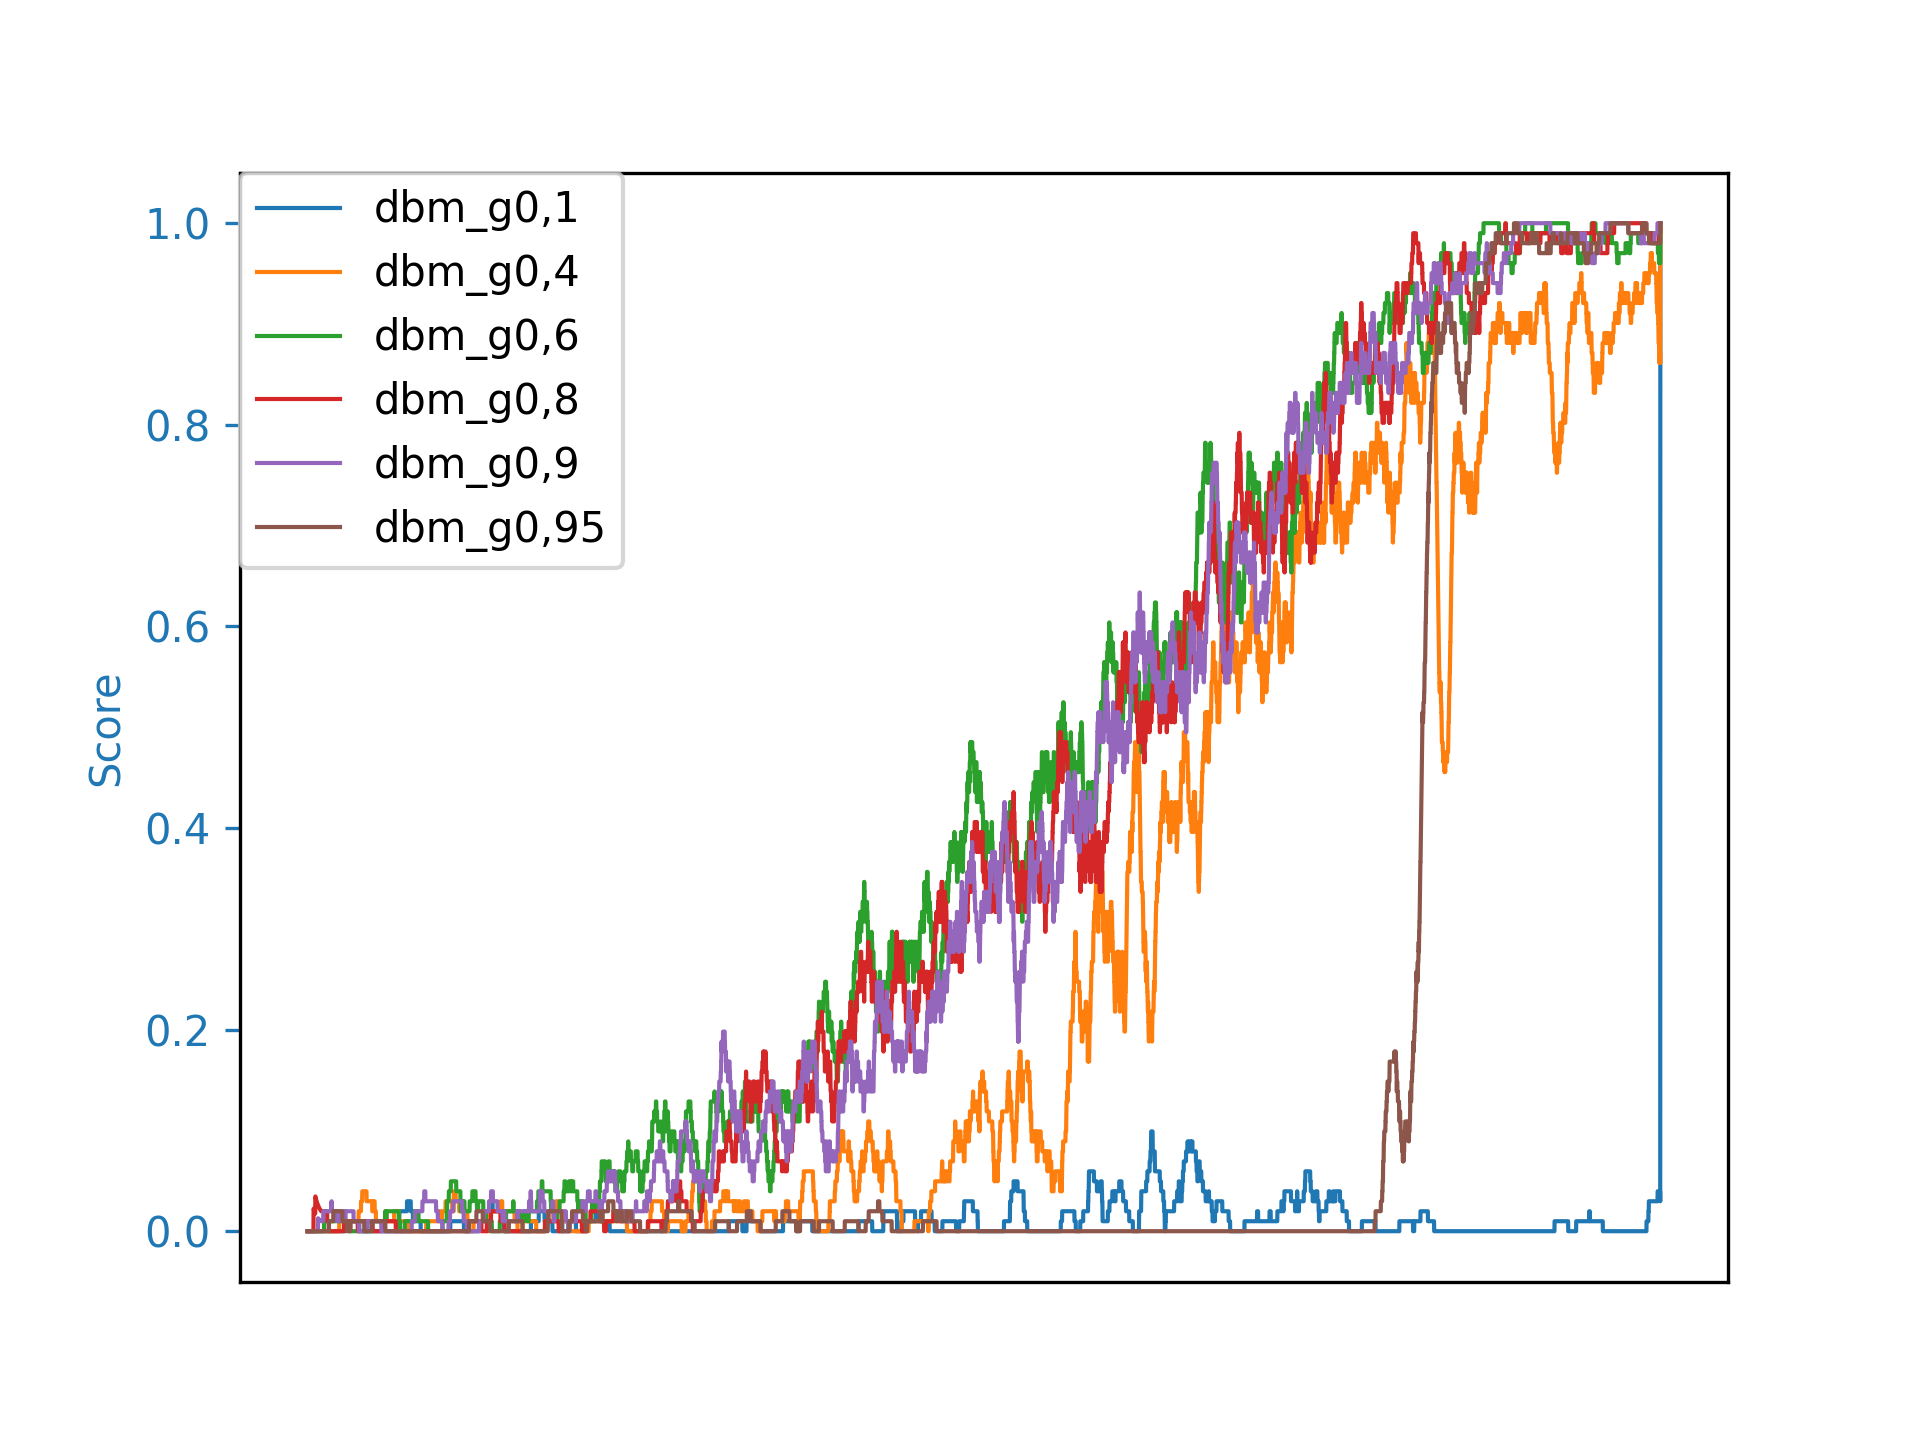
\includegraphics[width=\textwidth]{Figures/dbm5_4x4_dbm_g0,1_dbm_g0,4_dbm_g0,6_dbm_g0,8_dbm_g0,9_dbm_g0,95.png}
\caption{4x4 Tiefe Boltzmann maschine: $\gamma$}
\label{dbm1}
\end{figure}

Hier sind die Ergebnisse ähnlich wie bei der beschränkten Boltzmann Maschine. Zwischen 0,6 und 0,9 sind die Resultate gut. Daher bleiben wir hier wie auch in \citep{crawford2019reinforcement} bei $\gamma = 0.8$. Wir können hier im Hinterkopf behalten, dass größere Spielfelder eventuell mit höheren $\gamma$ Werten besser funktionieren. Anschaulich macht das Sinn, da der erwartete Gewinn über eine längere Kette von Aktionen bis zum Startfeld erhalten bleiben soll. Man kann diesen Effekt bei dem Vergleich zwischen dem 3x3 und dem 4x4 Feld auch erkennen.

Als nächstes testen wir $\beta$. Wie auch zuvor schon erwähnt, gibt es hier eine Variante dbm\_ , welche den Entropy Term komplett weglässt.

\begin{figure}[H]
\centering
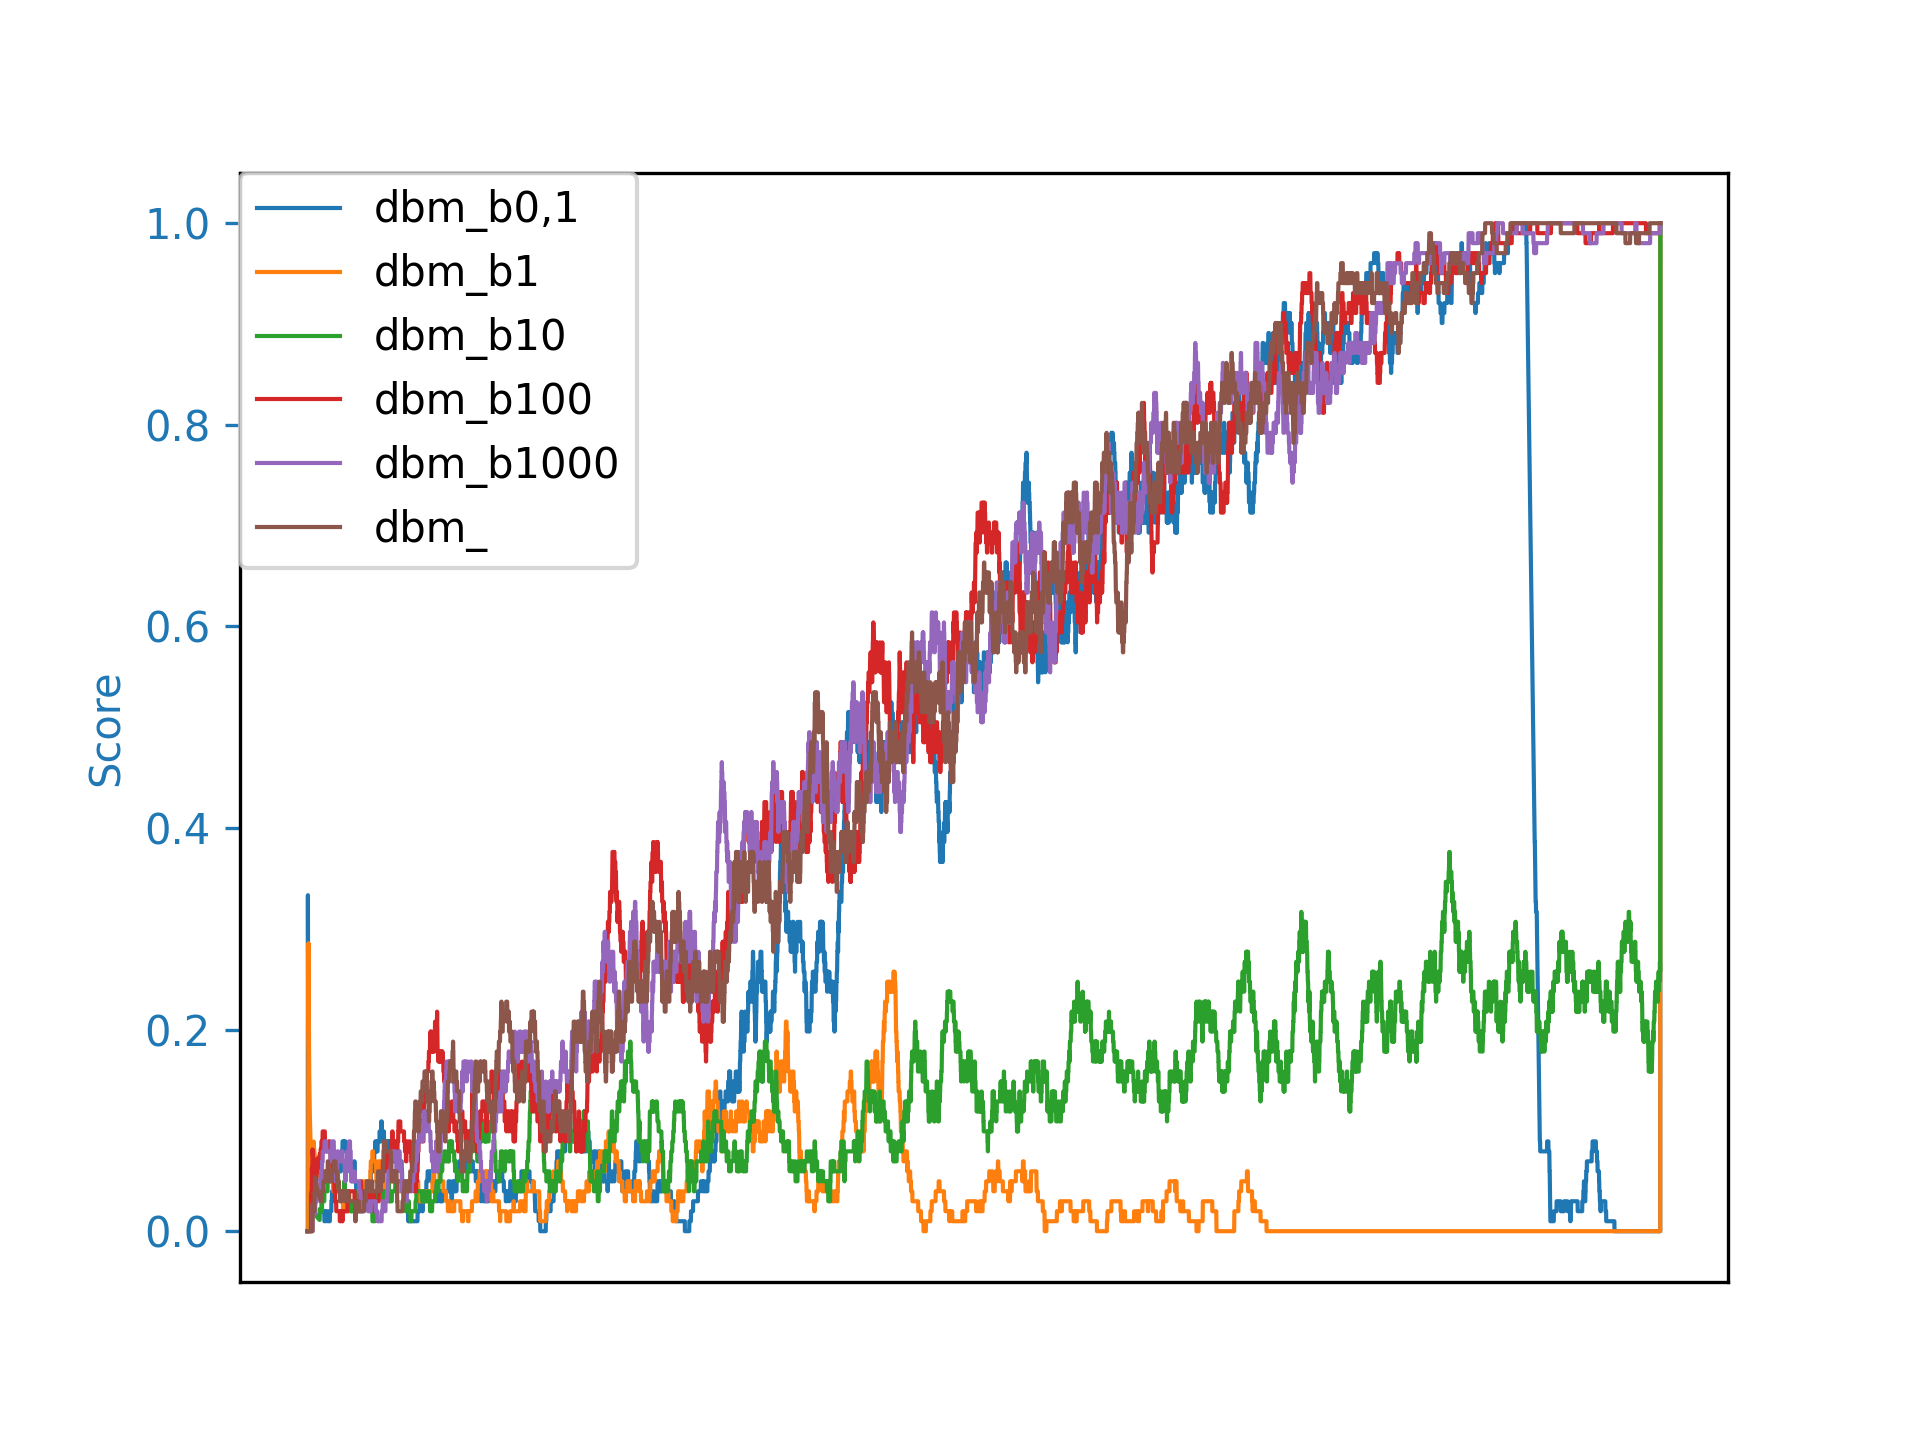
\includegraphics[width=\textwidth]{Figures/dbm2_3x3_dbm_b0,1_dbm_b1_dbm_b10_dbm_b100_dbm_b1000_dbm_.png}
\caption{3x3 Tiefe Boltzmann maschine: $\beta$}
\label{dbm1}
\end{figure}

\begin{figure}[H]
\centering
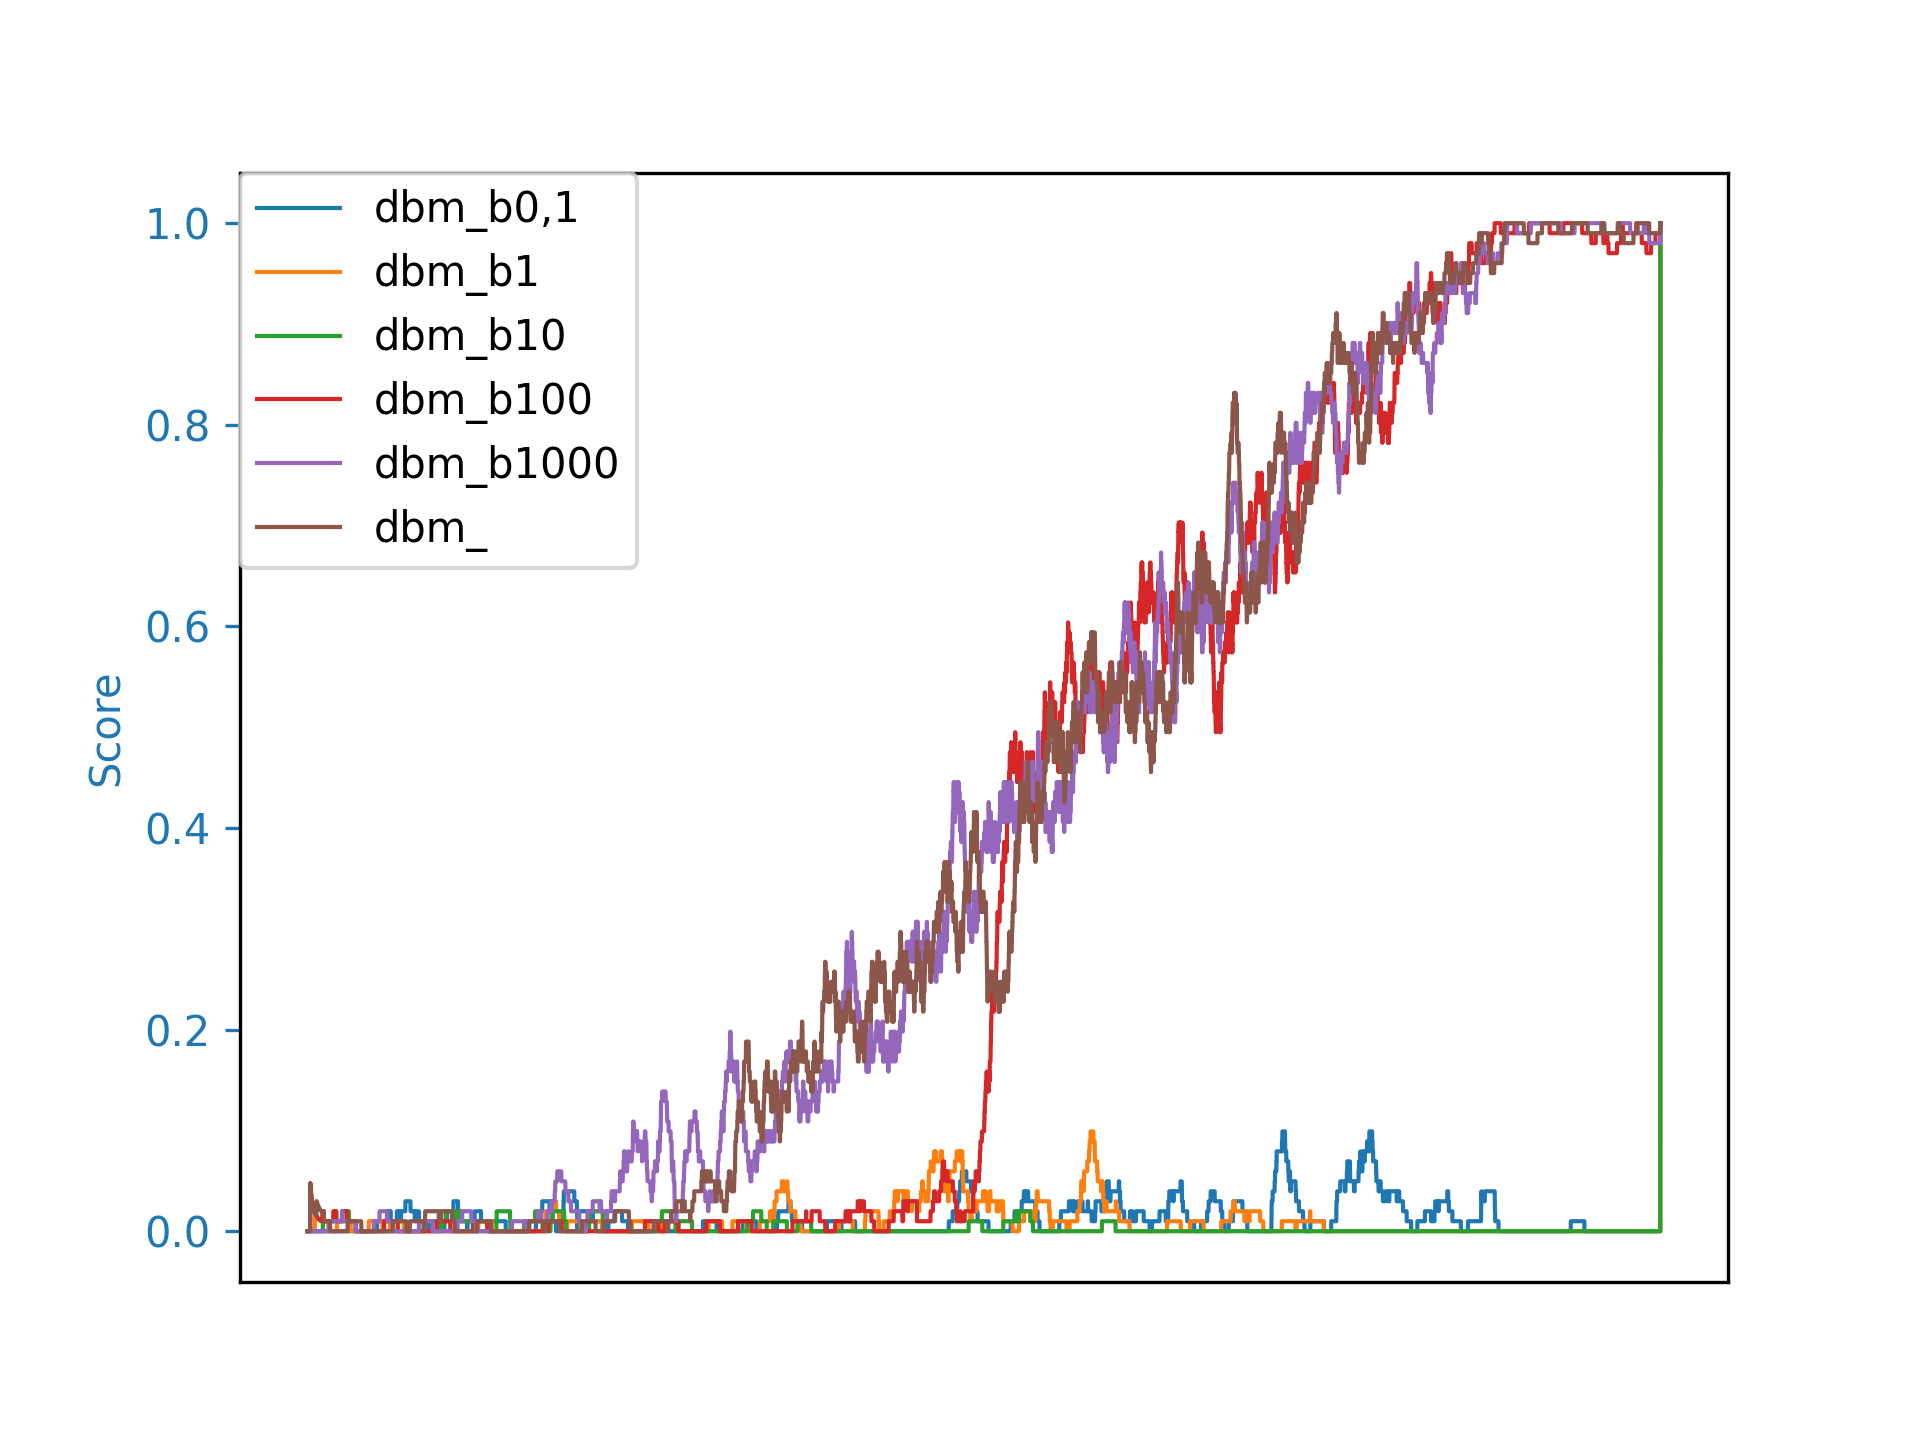
\includegraphics[width=\textwidth]{Figures/dbm3_4x4_dbm_b0,1_dbm_b1_dbm_b10_dbm_b100_dbm_b1000_dbm_.png}
\caption{4x4 Tiefe Boltzmann maschine: $\beta$}
\label{dbm1}
\end{figure}

Wir sehen also hier, je höher der Wert für $\beta$ umso besser die Ergebnisse. $\beta$ ist dabei der Faktor, durch den der Entropy-Term geteilt wird. Also ein sehr hoher Wert für $\beta$ reduziert den Einfluss von diesem Term. Werte wie 1000 sind dabei so groß, dass der Term quasi keinen Einfluss mehr hat. Man sieht hier auch, dass die Variante dbm\_ ohne die Entropy vergleichbare Ergebnisse erzielt wie sehr hohe $\beta$ Werte. Infolgedessen können wir ab hier den Entropy-Term komplett weglassen.

Als nächstes testen wir die Lernrate:

\begin{figure}[H]
\centering
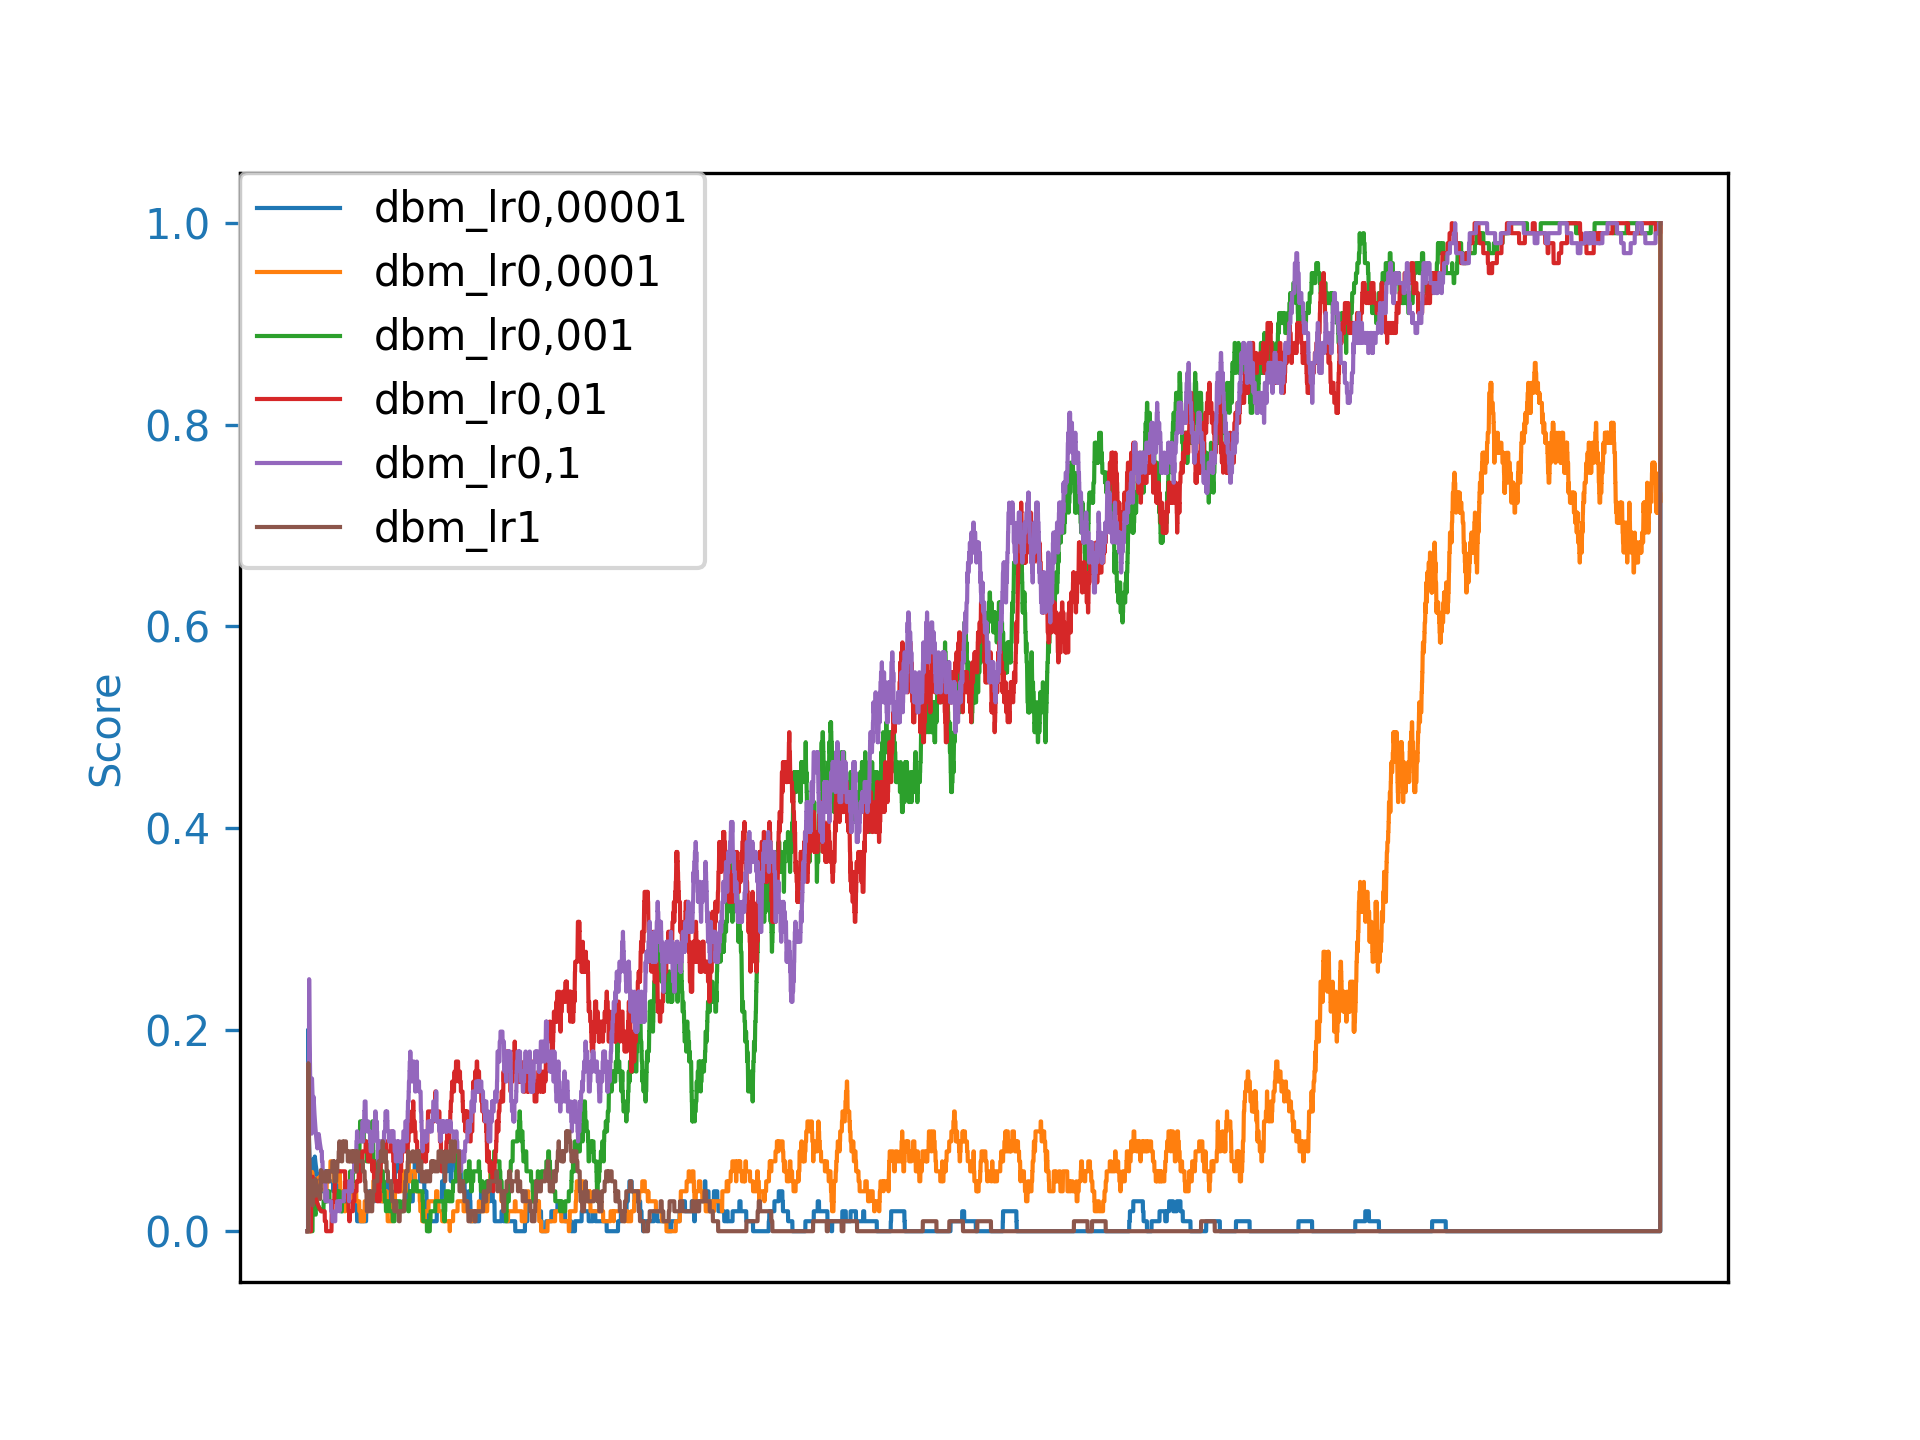
\includegraphics[width=\textwidth]{Figures/dbm6_3x3_dbm_lr0,00001_dbm_lr0,0001_dbm_lr0,001_dbm_lr0,01_dbm_lr0,1_dbm_lr1.png}
\caption{3x3 Tiefe Boltzmann maschine: $\beta$}
\label{dbm1}
\end{figure}

\begin{figure}[H]
\centering
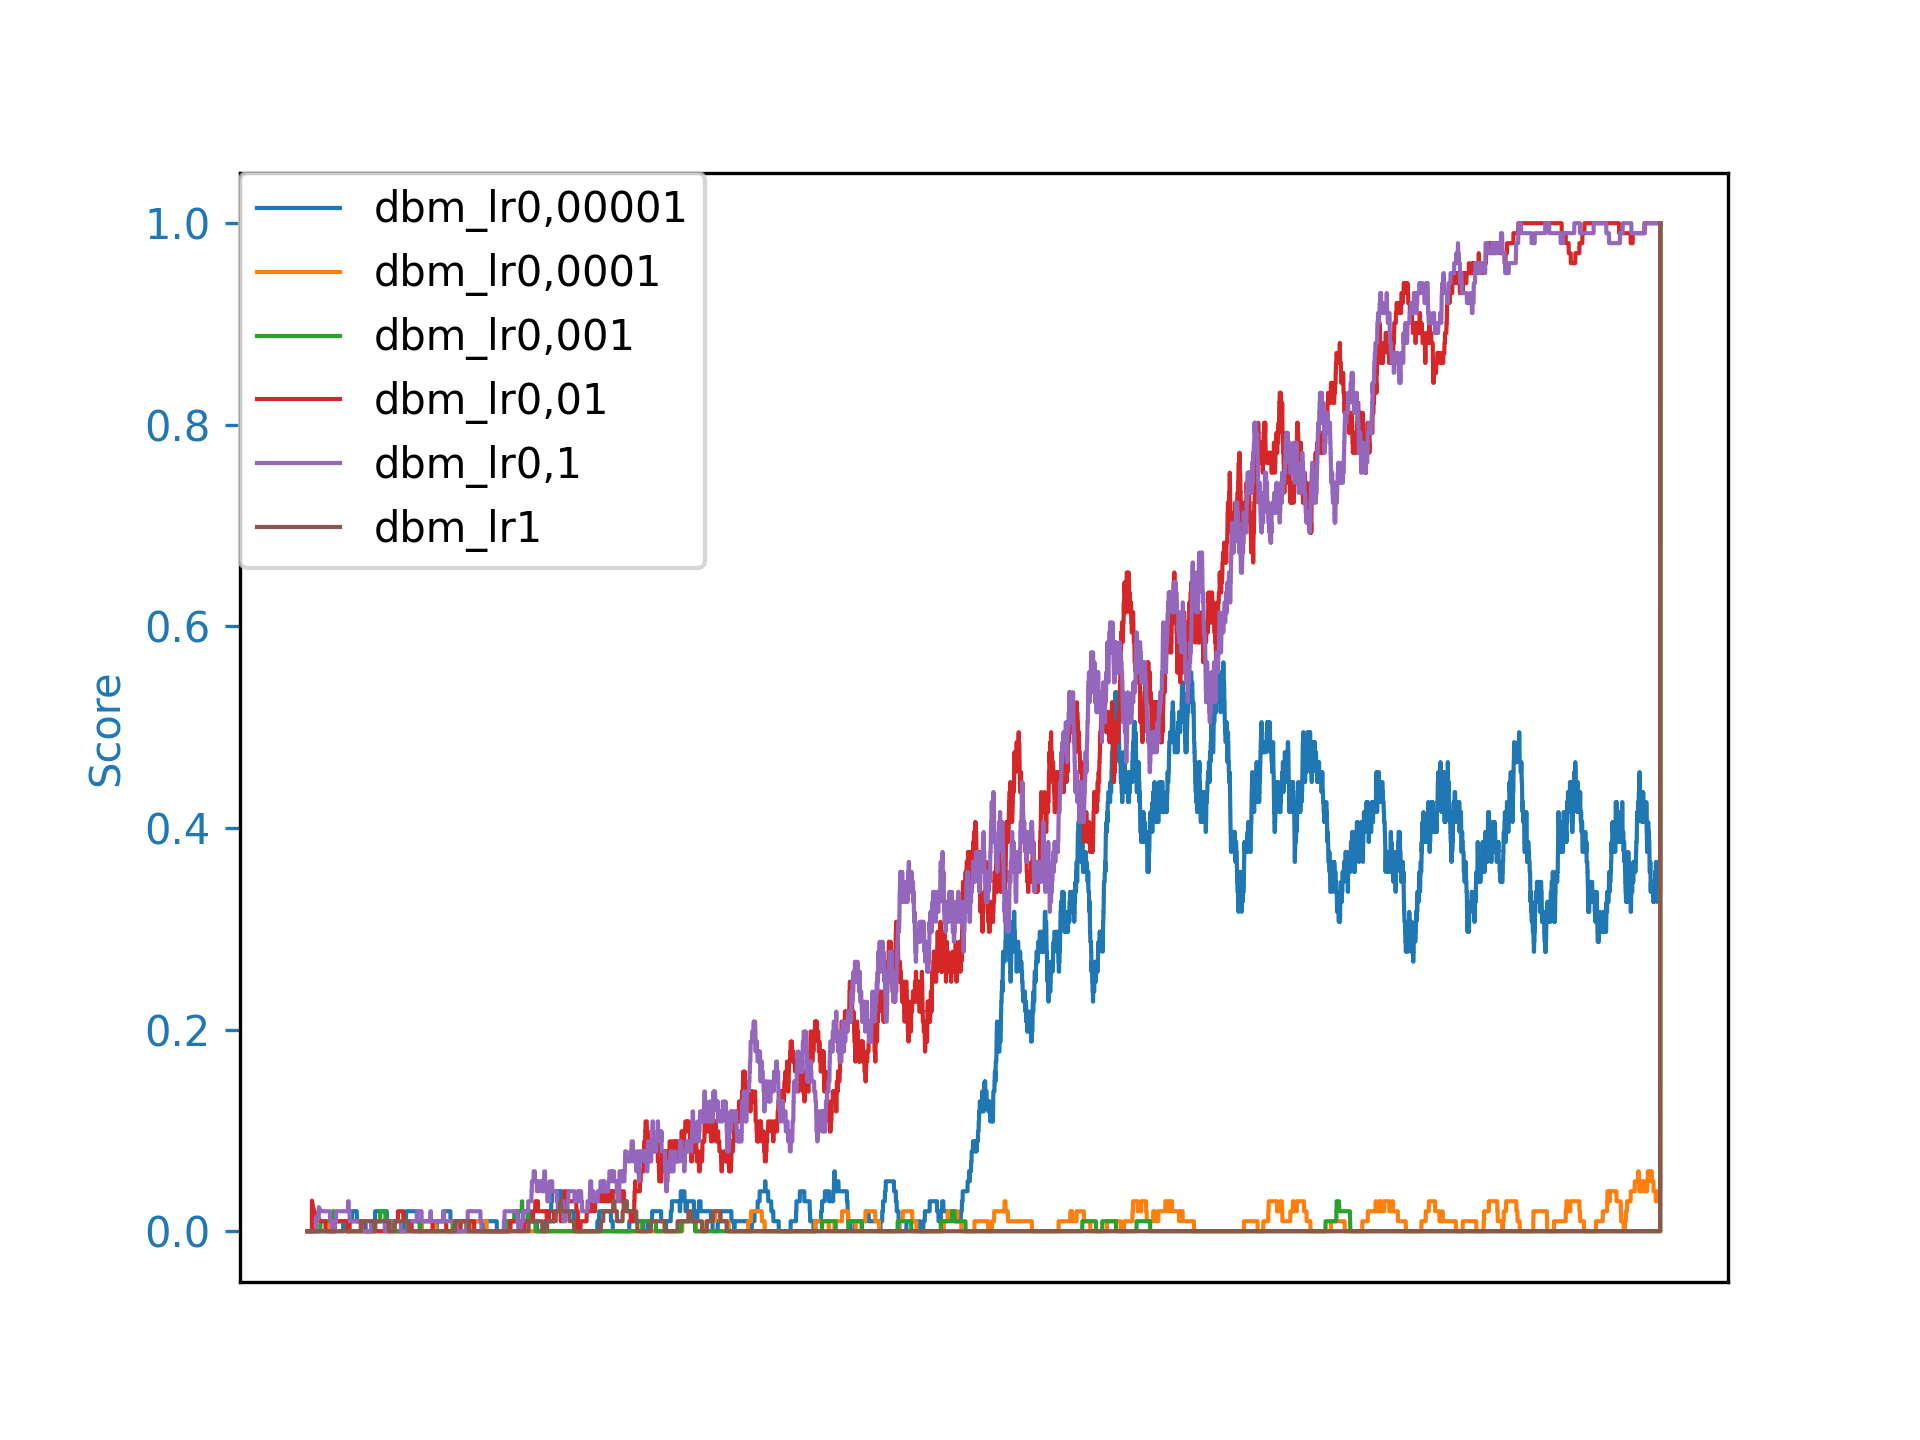
\includegraphics[width=\textwidth]{Figures/dbm7_4x4_dbm_lr0,00001_dbm_lr0,0001_dbm_lr0,001_dbm_lr0,01_dbm_lr0,1_dbm_lr1.png}
\caption{4x4 Tiefe Boltzmann maschine: $\beta$}
\label{dbm1}
\end{figure}

Am besten schneiden hier die Werte 0,1 und 0,01 ab. Wir entscheiden uns daher im weiteren einen mittleren Wert von 0,05 zu benutzen.

Schauen wir uns nun die Standardabweichung an, mit der wir die Gewichte initialisieren:

\begin{figure}[H]
\centering
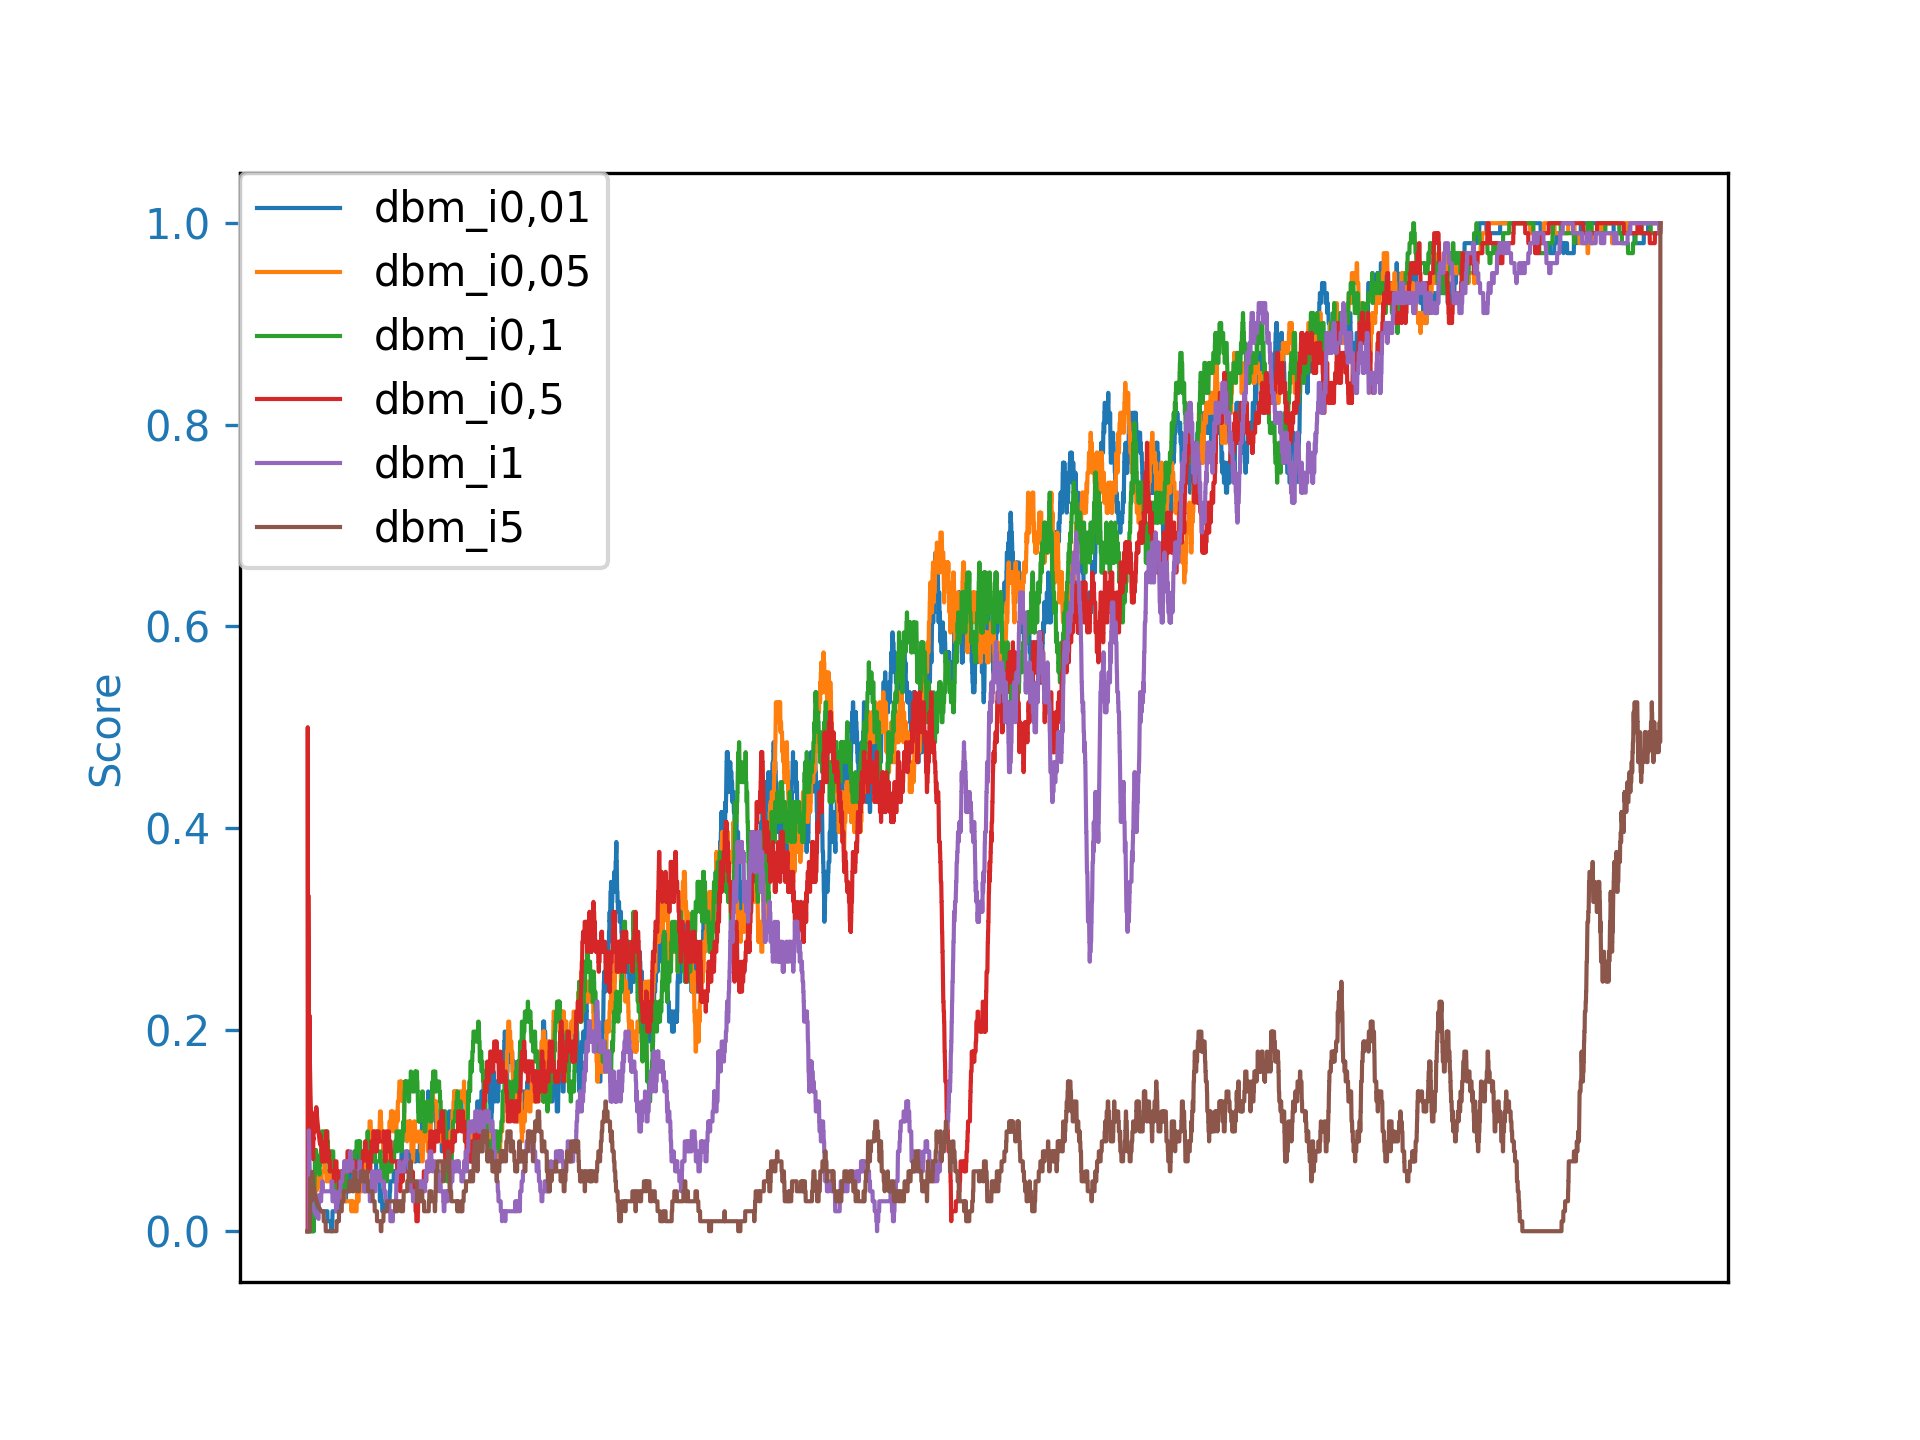
\includegraphics[width=\textwidth]{Figures/dbm8_3x3_dbm_i0,01_dbm_i0,05_dbm_i0,1_dbm_i0,5_dbm_i1_dbm_i5.png}
\caption{3x3 Tiefe Boltzmann maschine: $\beta$}
\label{dbm1}
\end{figure}

\begin{figure}[H]
\centering
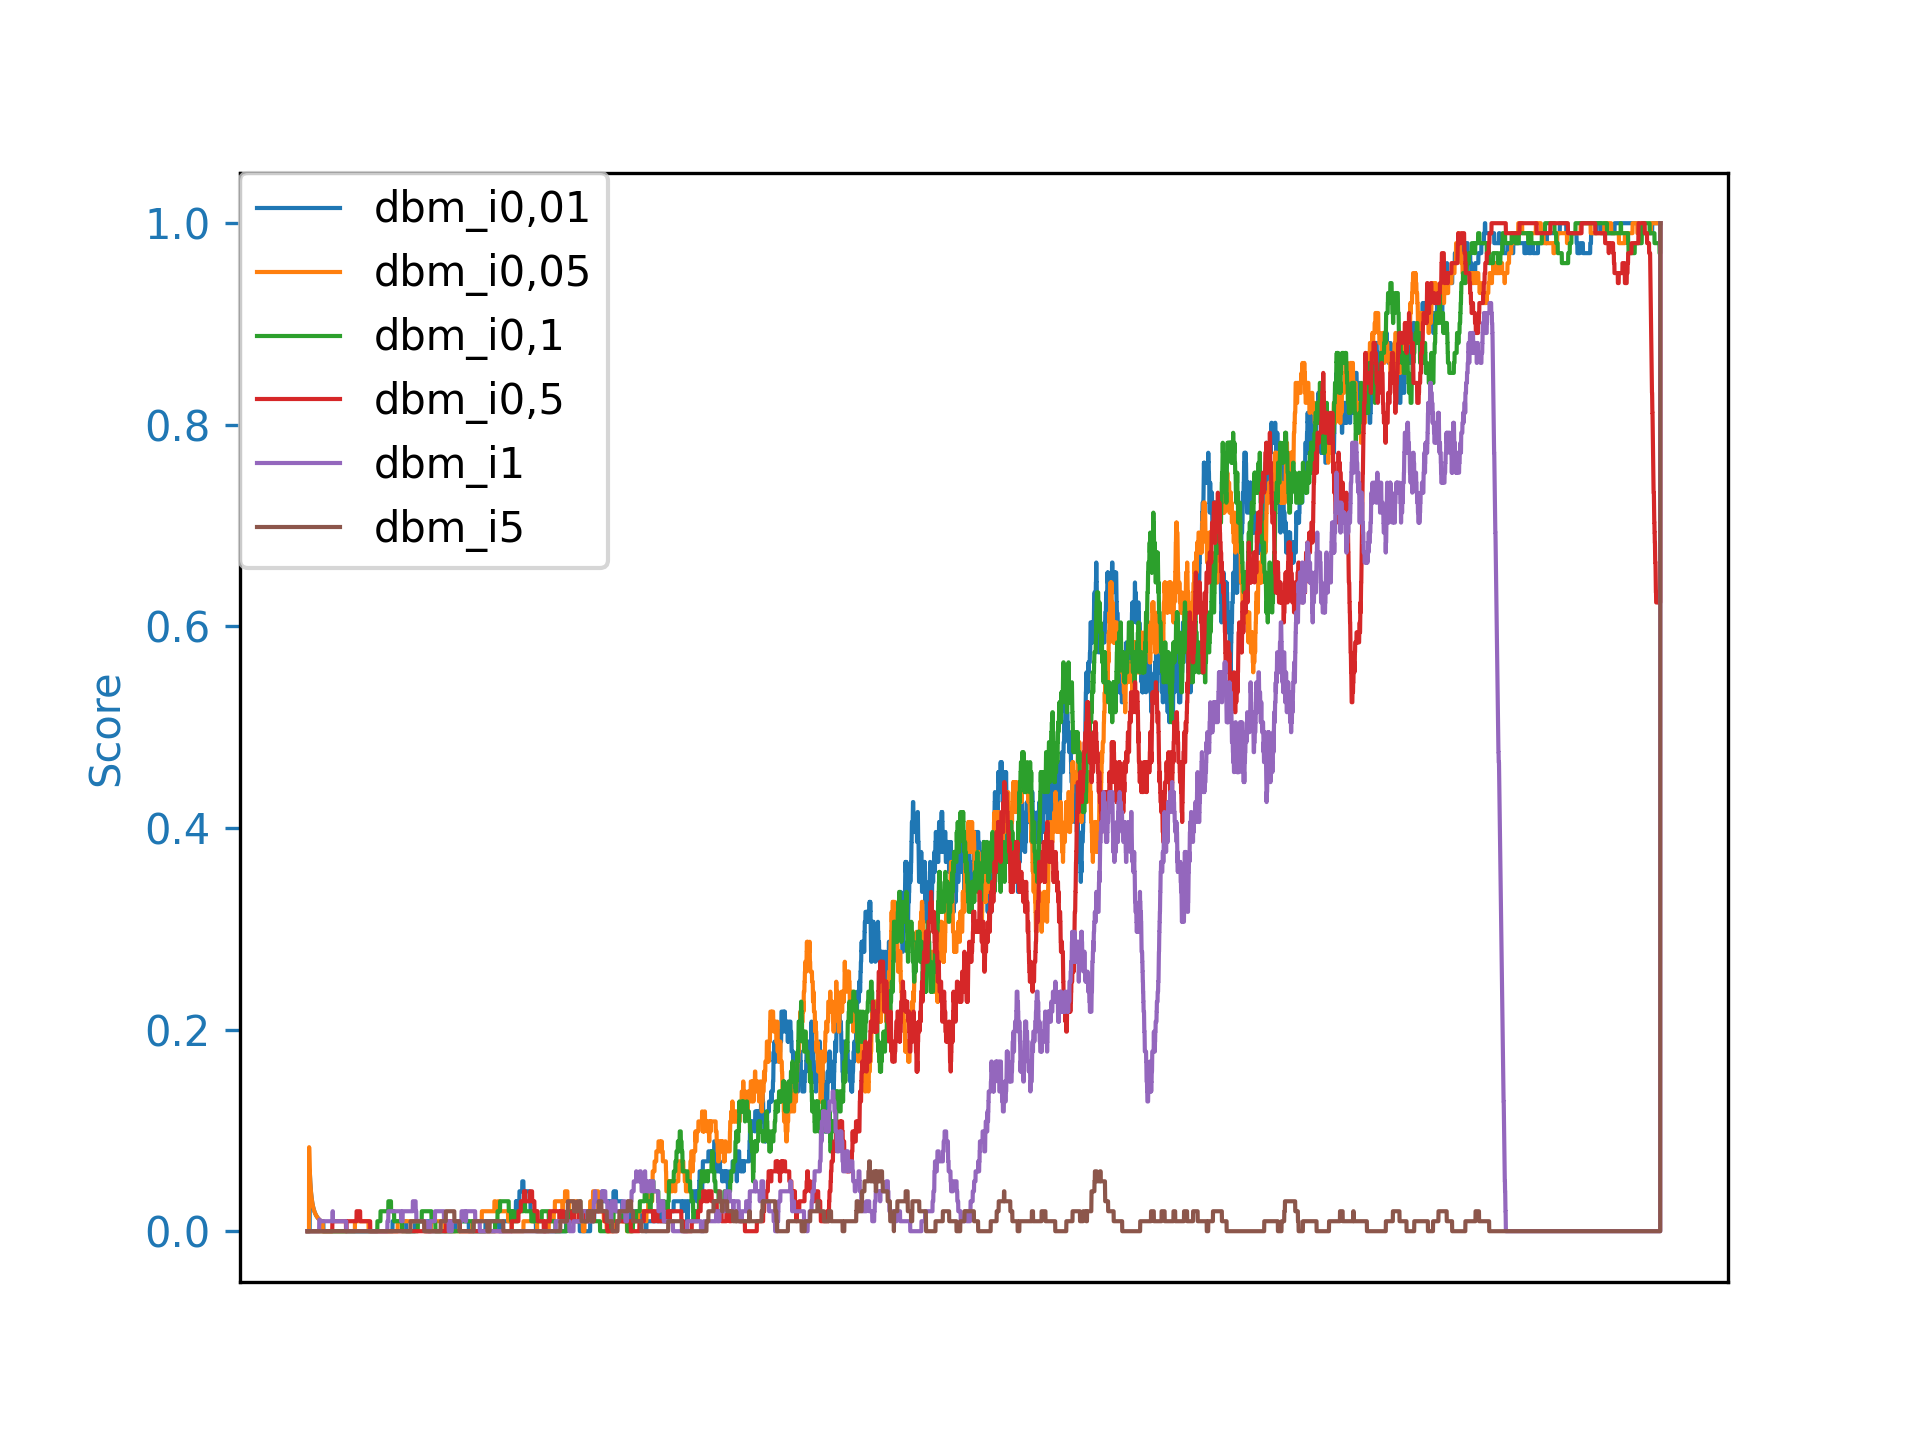
\includegraphics[width=\textwidth]{Figures/dbm9_4x4_dbm_i0,01_dbm_i0,05_dbm_i0,1_dbm_i0,5_dbm_i1_dbm_i5.png}
\caption{4x4 Tiefe Boltzmann maschine: $\beta$}
\label{dbm1}
\end{figure}

Hier scheinen vor allem kleine Werte gut zu funktionieren. Wir wählen im Folgenden 0,05, da dieser Wert gute Ergebnisse liefert.

Als letztes wollen wir noch die Annealing Temperatur testen. Dies gestaltet sich von allem Parametern am schwierigsten. Zum einen müssen wir hier drei Werte im Auge behalten: Den Startwert, den Endwert und das Verhältnis von beiden. Zum anderen liefern hier viele Werte gute Ergebnisse. Daher schauen wir uns gleich das 5x5 Spielfeld an. Hier ist es aber so schwierig, überhaupt das Ziel zu finden, dass die Ergebnisse ein wenig vom Zufall abhängen. Daher wollen wir hier keine Graphen von einzelnen Durchläufen zeigen, sondern die Azahl der richtige Policen die mit den drei oben genannten Werten gefunden wurden, in einer Tabelle aufzeigen:

\begin{table}[H]
	\centering
	\begin{tabular}{c|c}
	Startwert		& Richtige Policen	\\
	\hline
	0,001		& 	0 / 1			\\
	\hline
	0,01			& 	4 / 7			\\
	\hline
	0,1			& 	5 / 13		\\
	\hline
	1			& 	6 / 12		\\
	\hline
	10 			&	11 / 13		\\
	\hline
	100			&	5 / 8			\\
	\hline
	1000			&	2 / 3
	\end{tabular}
\end{table} 

\begin{table}[H]
	\centering
	\begin{tabular}{c|c}
	Endwert		& Richtige Policen	\\
	\hline
	0,2			&	0 / 1			\\
	\hline
	0,5			&	0 / 2			\\
	\hline
	1			& 	0 / 6			\\
	\hline
	2			& 	1 / 2			\\
	\hline
	5			& 	0 / 2			\\
	\hline
	10			& 	4 / 5			\\
	\hline
	20			& 	2 / 2			\\
	\hline
	50			& 	2 / 3			\\
	\hline
	100			& 	7 / 9			\\
	\hline
	200			& 	1 / 1			\\
	\hline
	500			& 	1 / 2			\\
	\hline
	1000			& 	7 / 10		\\
	\hline
	5000			& 	1 / 2			\\
	\hline
	10 000		&	6 / 9			\\
	\hline
	100 000		&	1 / 1
	\end{tabular}
\end{table} 

\begin{table}[H]
	\centering
	\begin{tabular}{c|c}
	Verhältnis		& Richtige Policen	\\
	\hline
	1 zu 2		&	4 / 6			\\
	\hline
	1 zu 5		&	3 / 7			\\
	\hline
	1 zu 10		& 	7 / 13		\\
	\hline
	1 zu 50		& 	1 / 4			\\
	\hline
	1 zu 100		& 	8 / 12		\\
	\hline
	1 zu 1000		& 	2 / 5			\\
	\hline
	1 zu 10000		& 	6 / 7			\\
	\hline
	1 zu 100000	& 	1 / 2			\\
	\hline
	1 zu 1000000	& 	1 / 1
	\end{tabular}
\end{table} 

Insgesamt haben wir also 57 Strategien getestet und dabei 33 mal die richtige Police gefunden. Das entspricht 58\%. Allerdings ist es garnicht einfach, die Ergebnisse zu interpretieren. Wir testen also am besten mehrere Varianten von guten Parametern mit mehreren Durchläufen. 

Bei den Startwerten haben wir die besten Ergebnisse für 10. Bei den Endwerten scheinen tendenziell größere Werte besser zu funktionieren. Auch bei dem Verhältnis, sind größere Verhaltnisse in der Regel besser. \\

Wir wollen daher einen Testlauf mit dem Startwert 10 und dem besten Verhältnis 1 zu 10000 machen. So kommen wir auf die Parameter [10, 100000].
Einen zweiten Testlauf wollen wir mit dem besten Endwert machen. Dieser ist nicht ganz klar, wir wählen hier 100, da dieser Wert öfter getestet wurde. Was auch bei den Tests oft richtige Policen lieferte war [1, 100]. Wählen wir also diese Werte.
Und zuletzt wollen wir noch die Werte aus \citep{crawford2019reinforcement} mit [2, 20] testen.

Der Gewinner von diesen drei Vergleichen ist [2, 20] mit 27 von 30 richtigen Policen.
Platz 2 ist [10, 100000] mit 24 von 30. Und Letzter ist [1, 100] mit 20 von 30. Beachte aber das auch alle drei über den 58\% liegen, die wir in den gemischten Parametern erreicht haben.

Hier wäre es sicherlich noch spannend weiter zu testen. Vor allem fällt hier auf, das teilweise sehr kleine Verhältnisse wie bei [2, 20] gut funktionieren. Dann sind größere Verhältnisse wie 1 zu 1000 plötzlich schlecht und 1 zu 10000 funktioniert wieder gut. Hier scheint es keine lineare Abhängigkeit zu geben. \\

Fassen wir nun die besten Ergebnisse von allen Methoden zusammen und testen dann die Methoden gegeneinander.

\newpage

\subsection{Die besten Parameter}
\label{subsec:best}

Bevor wir die Ergebnisse von allen Methoden im Vergleich zeigen, hier eine Auflistung der besten Parameter aus den bisherigen Experimenten. Rbm steht für beschränkte Boltzmann Maschine und Qbm für die tiefe Boltzmann Maschine mit Quanten Annealing:

\begin{table}[H]
	\centering
	\begin{tabular}{c|c|c|c|c}
	Parameter 				& Q-Tabelle 	& Einfaches Netz 	& Rbm			 	& Qbm			  		\\
	\hline
	Lernrate 					& 0.1 		& 0.0001			& 0.01				& 0.05					\\
	\hline
	Neuronen 					& - 			& 16 - 64			& 64 	- $\infty$			& 8 - 32					\\
	\hline
	$\gamma$ 				& 0.8			& 0.4				& 0.8					& 0.8						\\
	\hline
	$\beta$ 					& - 			& - 				& 50 					& - 						\\
	\hline
	Initialwert 					& 0.5 		& - 				& 0 					& 0						\\
	\hline
	Std			 			& - 			& - 				& 1 					& 0.05					\\
	\hline
	Ann. runs					& - 			& - 				& - 					& 100 - $\infty$				\\
	\hline
	Ann. sweeps				& - 			& - 				& - 					& 100 - $\infty$				\\
	\hline
	Ann. Temp					& - 			& - 				& - 					& [2, 20]					\\
	\end{tabular}
\end{table} 

\subsection{Vergleich der Methoden gegeneinander}
\label{subsec:best_method}

Wir untersuchen als erstes 8 verschiedene Spielfelder in aufsteigender Größe und testen jeweils alle 4 Methoden. Die Spielfelder haben dabei die Größen 2x2, 3x3, 3x5, 4x4, 5x5, 6x6, 8x8 und 8x8. Dabei sind die beiden 8x8 Spielfelder nur noch mit wenigen Löchern versehen.

Bei der Anzahl an Neuronen haben wir hier noch etwas erhöht, da tendenziell bei größeren Spielfeldern mehr Neuronen gebraucht werden. Hier kommt das einfache Netz mit 32 Neuronen daher, die beschränkte Boltzmann Maschine mit 128 und die Quanten Boltzmann Maschine mit 16. Die Annealing Runs und Sweeps werden auf 200 gesetzt, für eine höhere Genauigkeit. Höhere Werte fürs Annealing sind leider aufgrund von der Rechenzeit auf meinem PC nicht möglich. Alle anderen Werte die benutzt wurden können 1 zu 1 auf der oben genannten Tabelle abgelesen werden.

\begin{figure}[H]
\centering
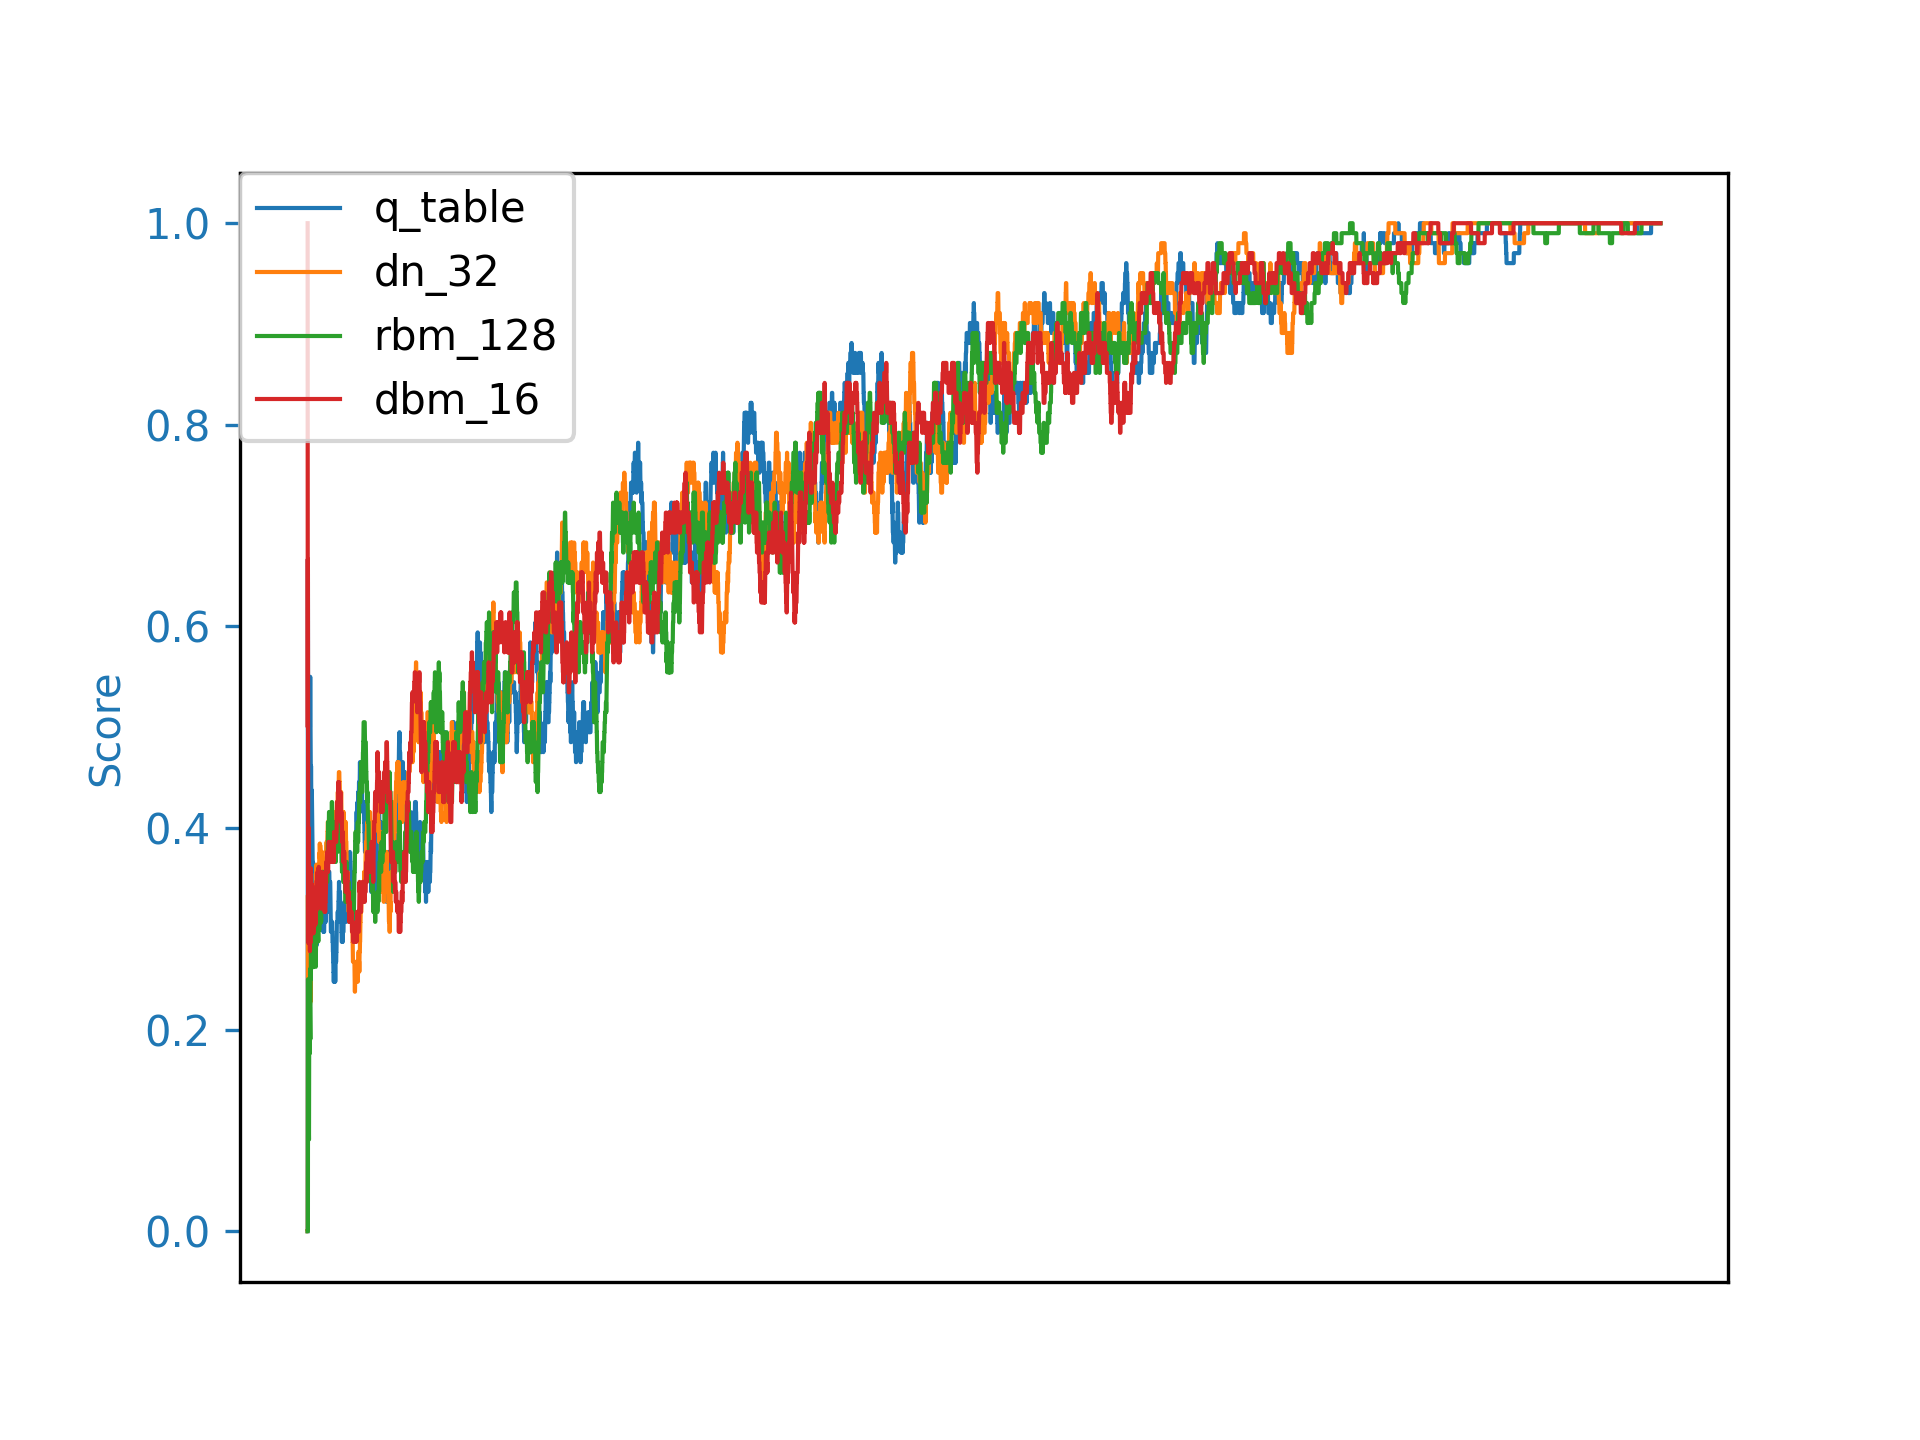
\includegraphics[width=\textwidth]{Figures/all_2x2_q_table_dn_32_rbm_128_dbm_16.png}
\caption{2x2 Alle Methoden}
\label{all_1}
\end{figure}

\begin{figure}[H]
\centering
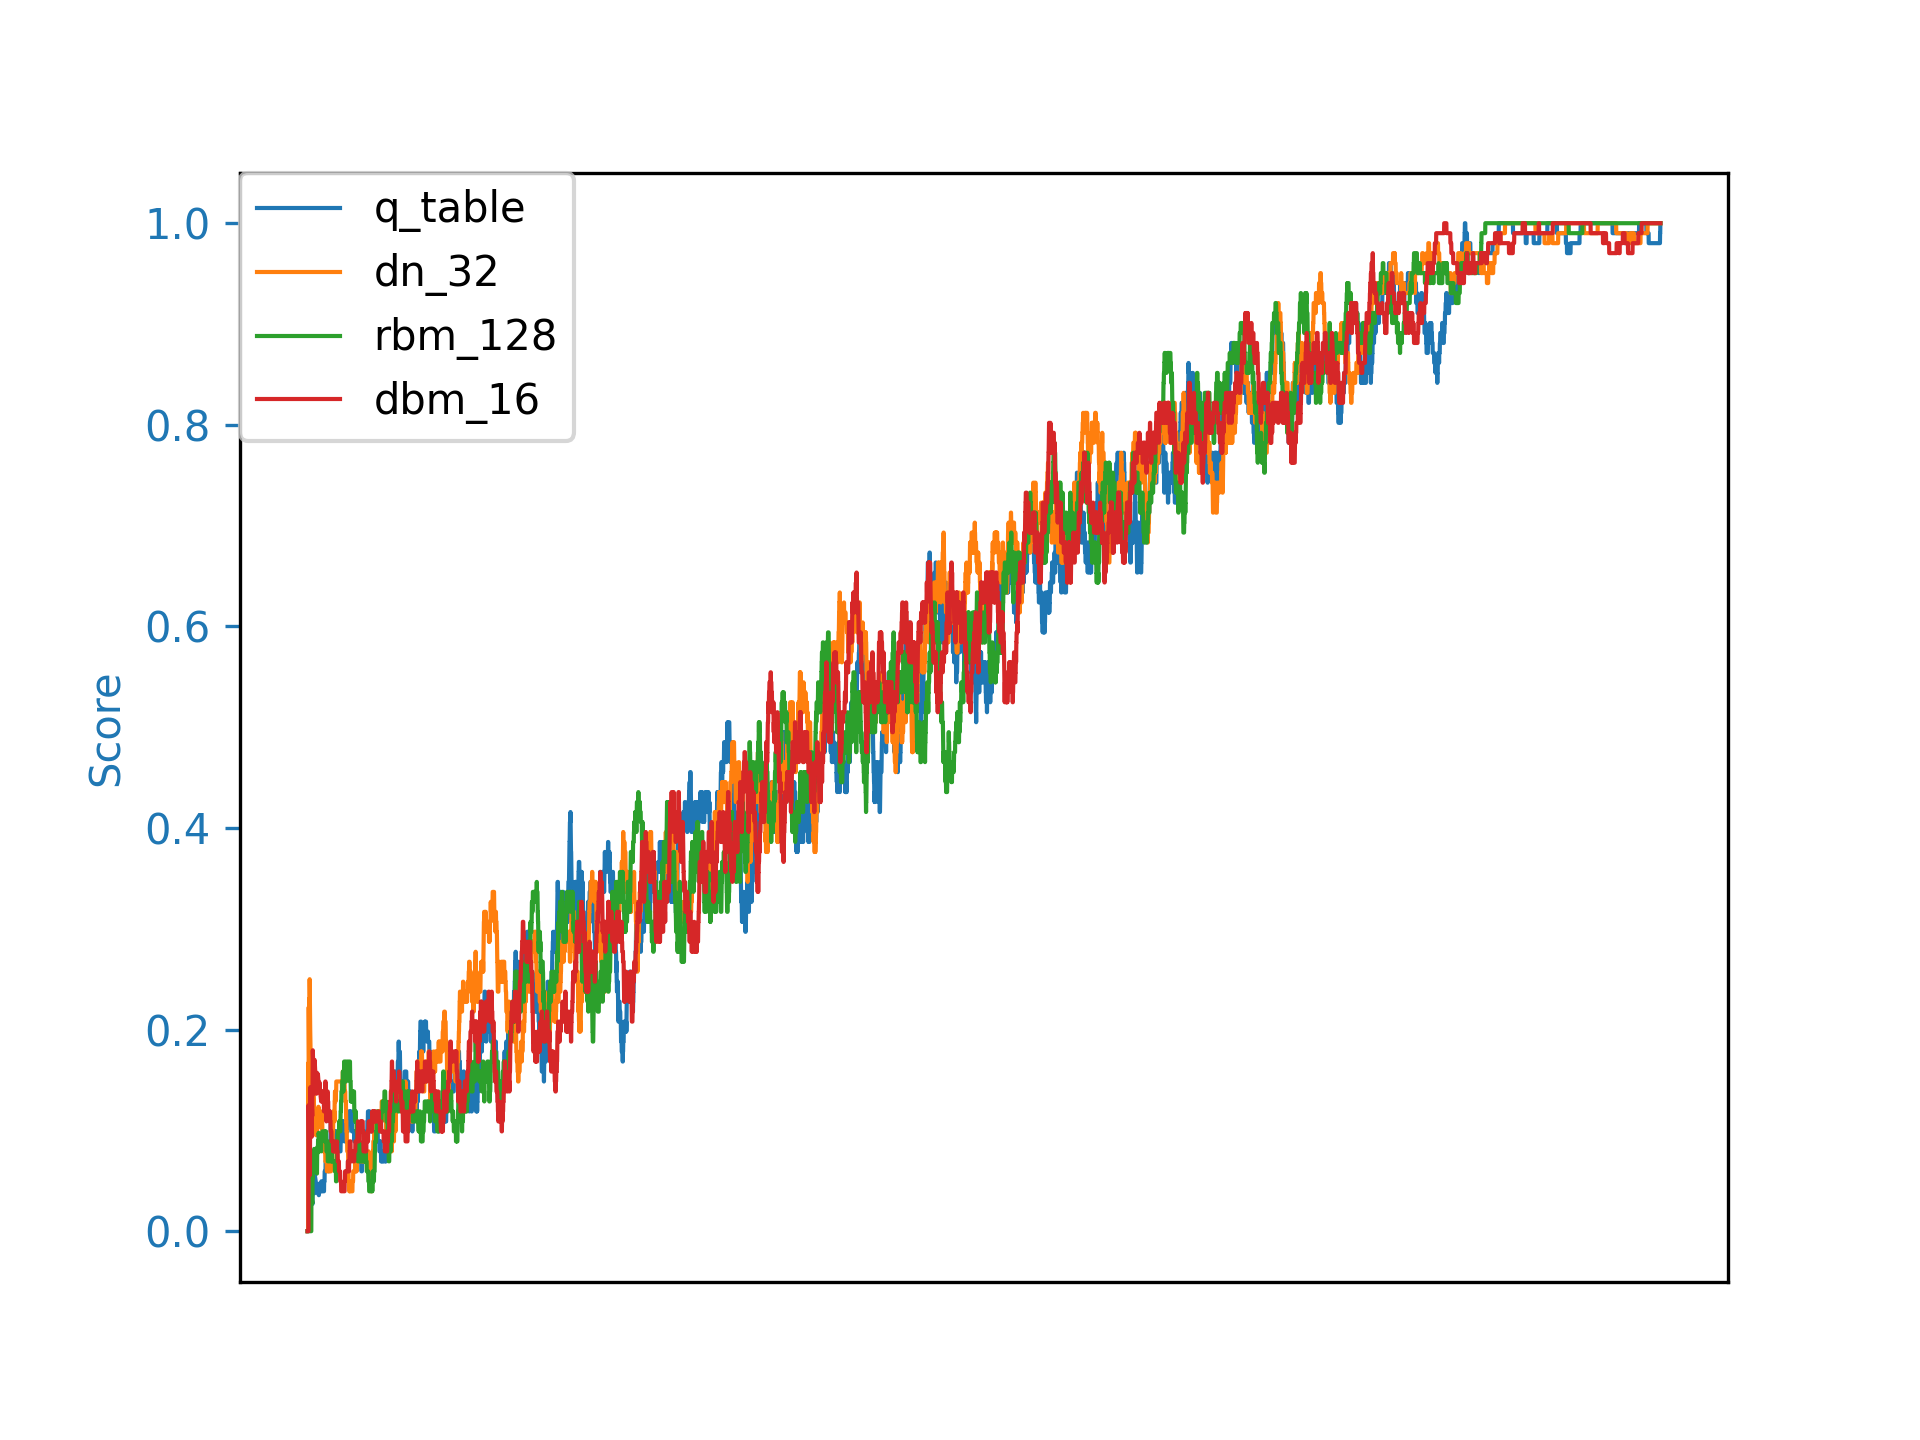
\includegraphics[width=\textwidth]{Figures/all_3x3_q_table_dn_32_rbm_128_dbm_16.png}
\caption{3x3 Alle Methoden}
\label{all_2}
\end{figure}

\begin{figure}[H]
\centering
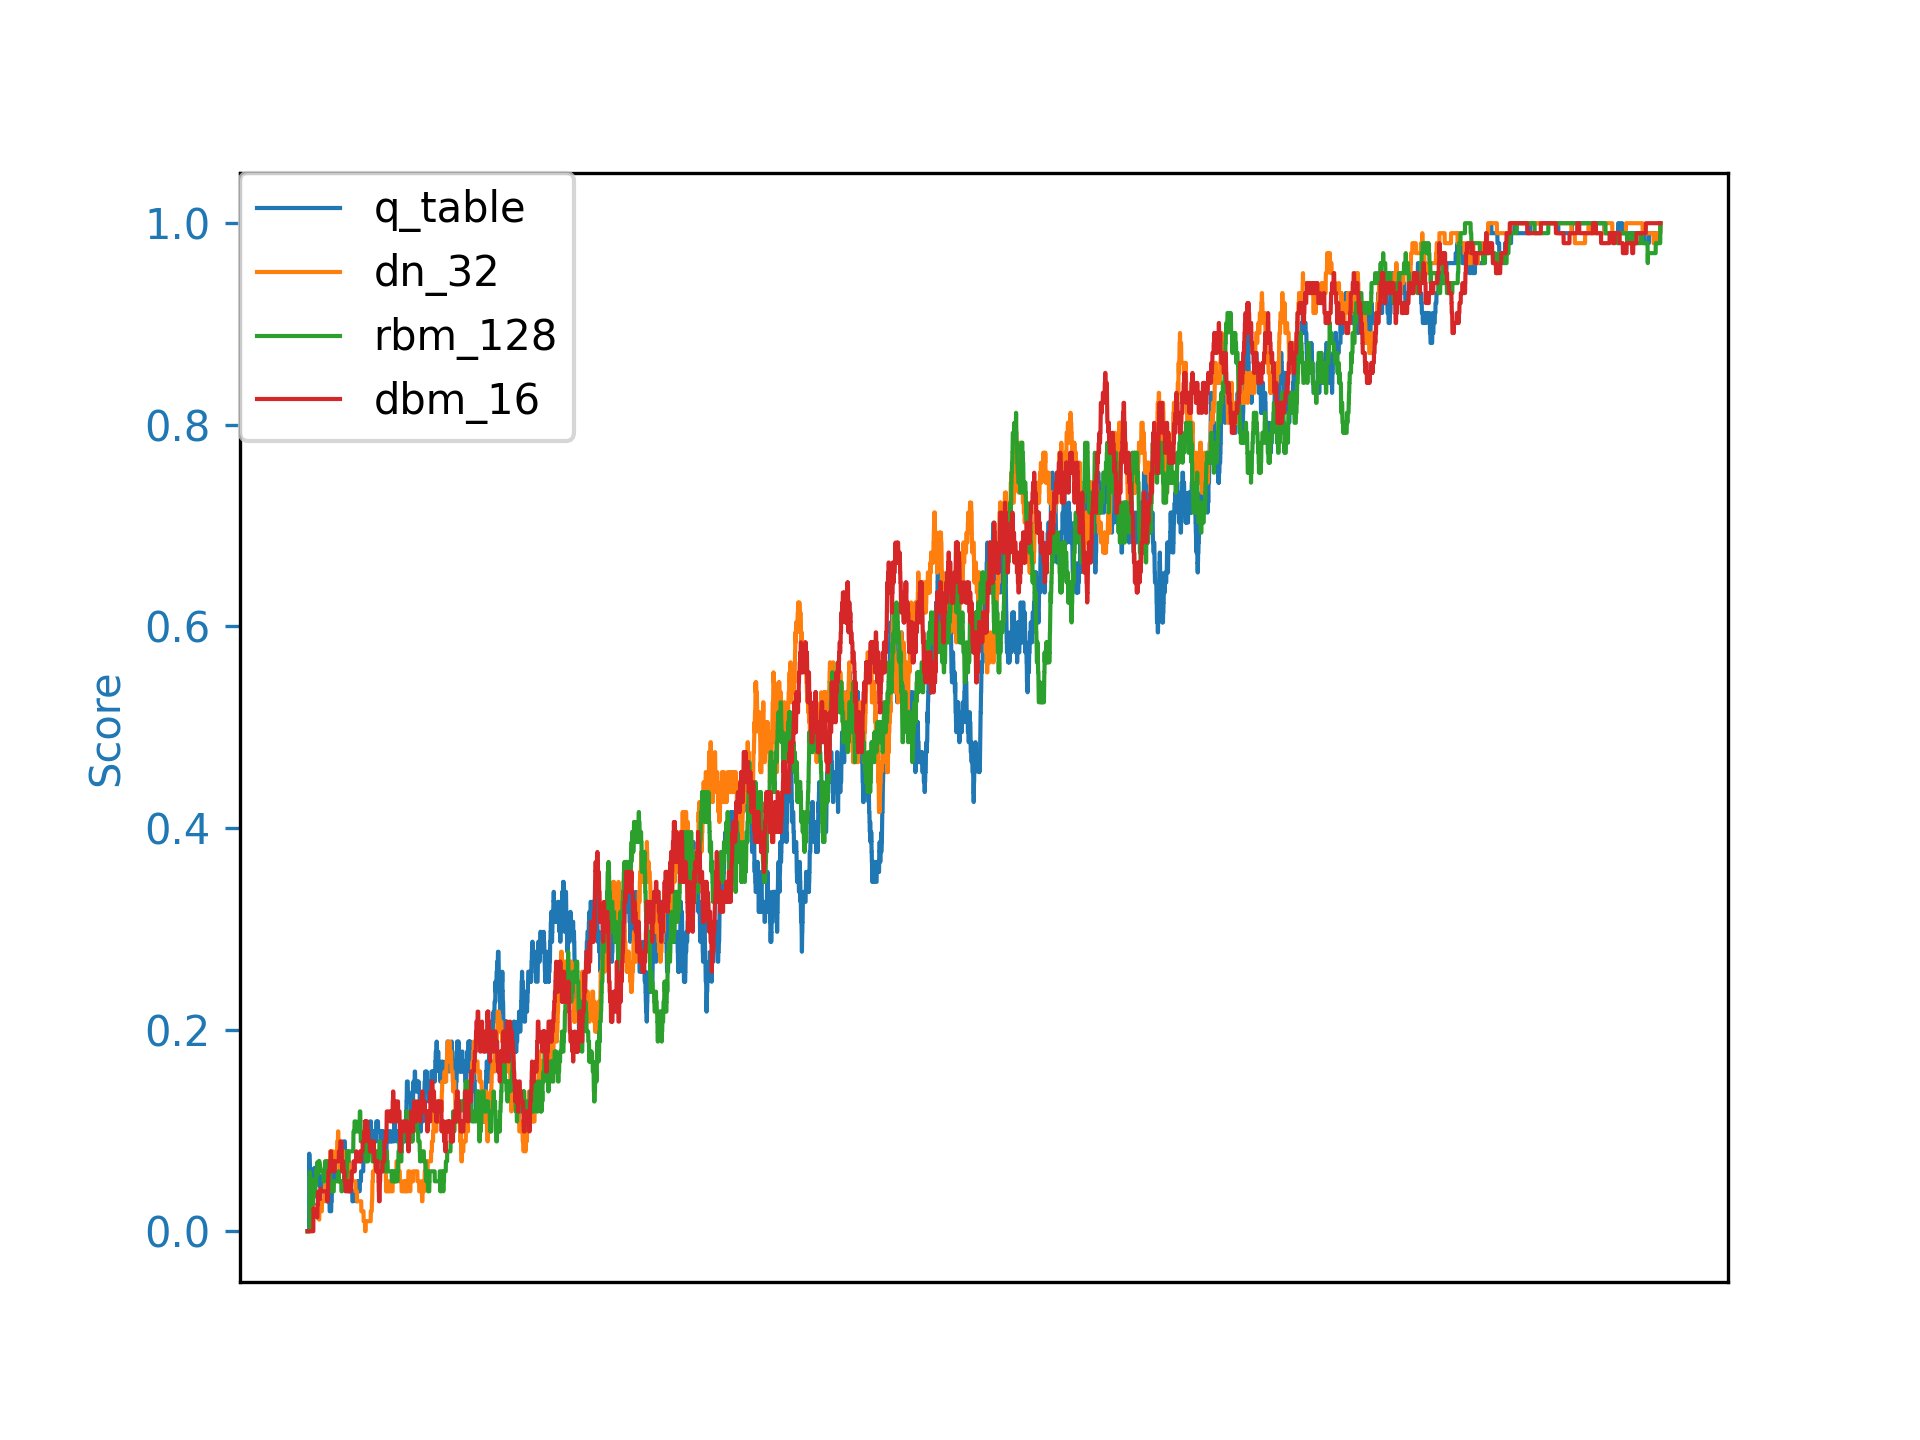
\includegraphics[width=\textwidth]{Figures/all_3x5_q_table_dn_32_rbm_128_dbm_16.png}
\caption{3x5 Alle Methoden}
\label{all_3}
\end{figure}

\begin{figure}[H]
\centering
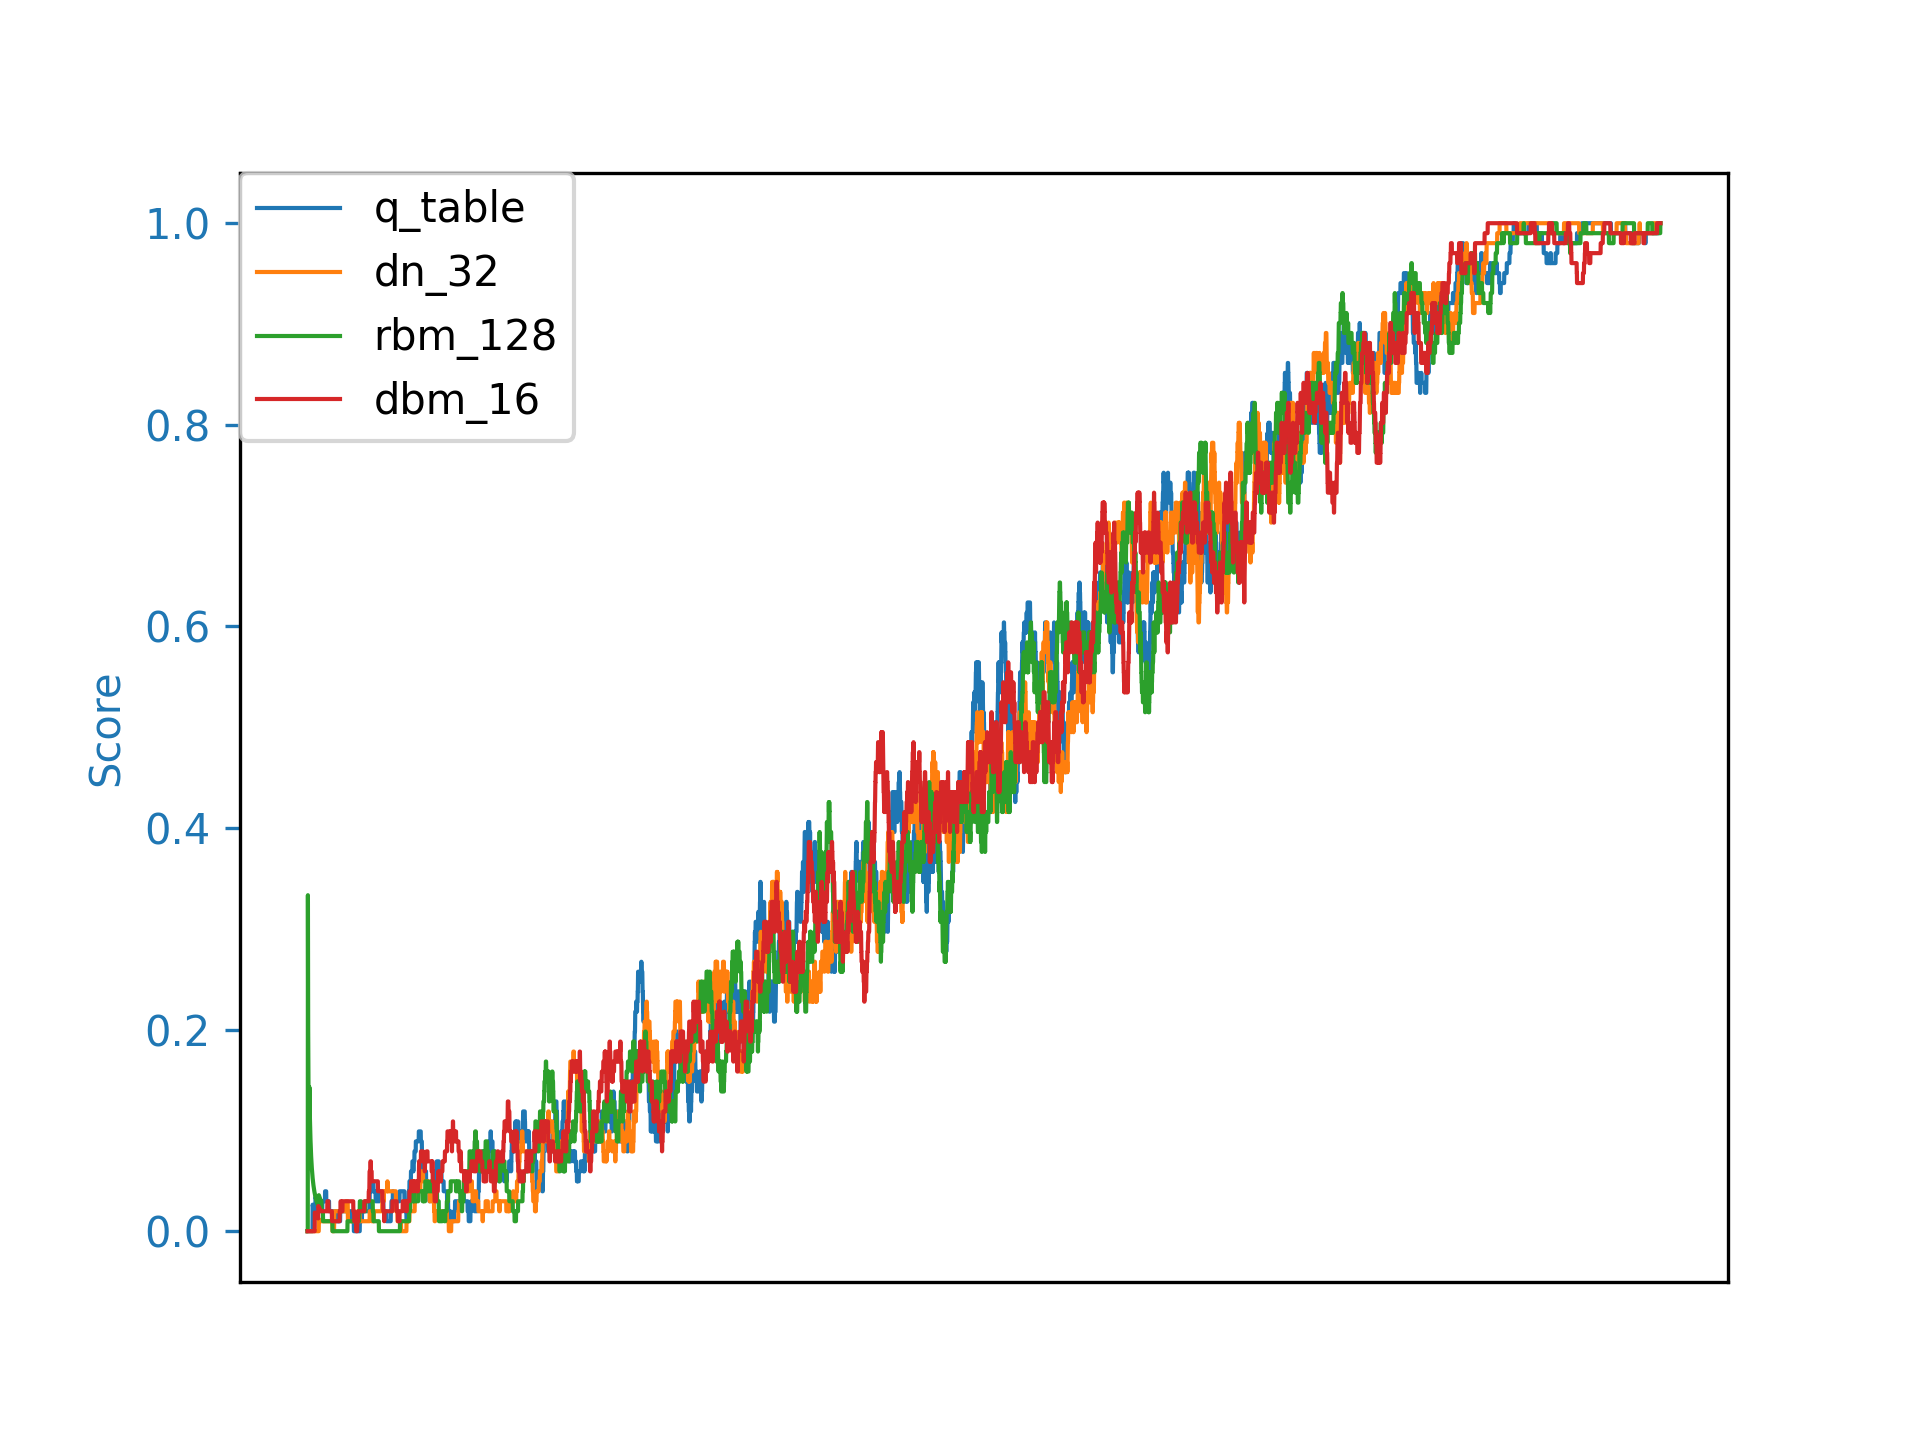
\includegraphics[width=\textwidth]{Figures/all_4x4_q_table_dn_32_rbm_128_dbm_16.png}
\caption{4x4 Alle Methoden}
\label{all_4}
\end{figure}

\begin{figure}[H]
\centering
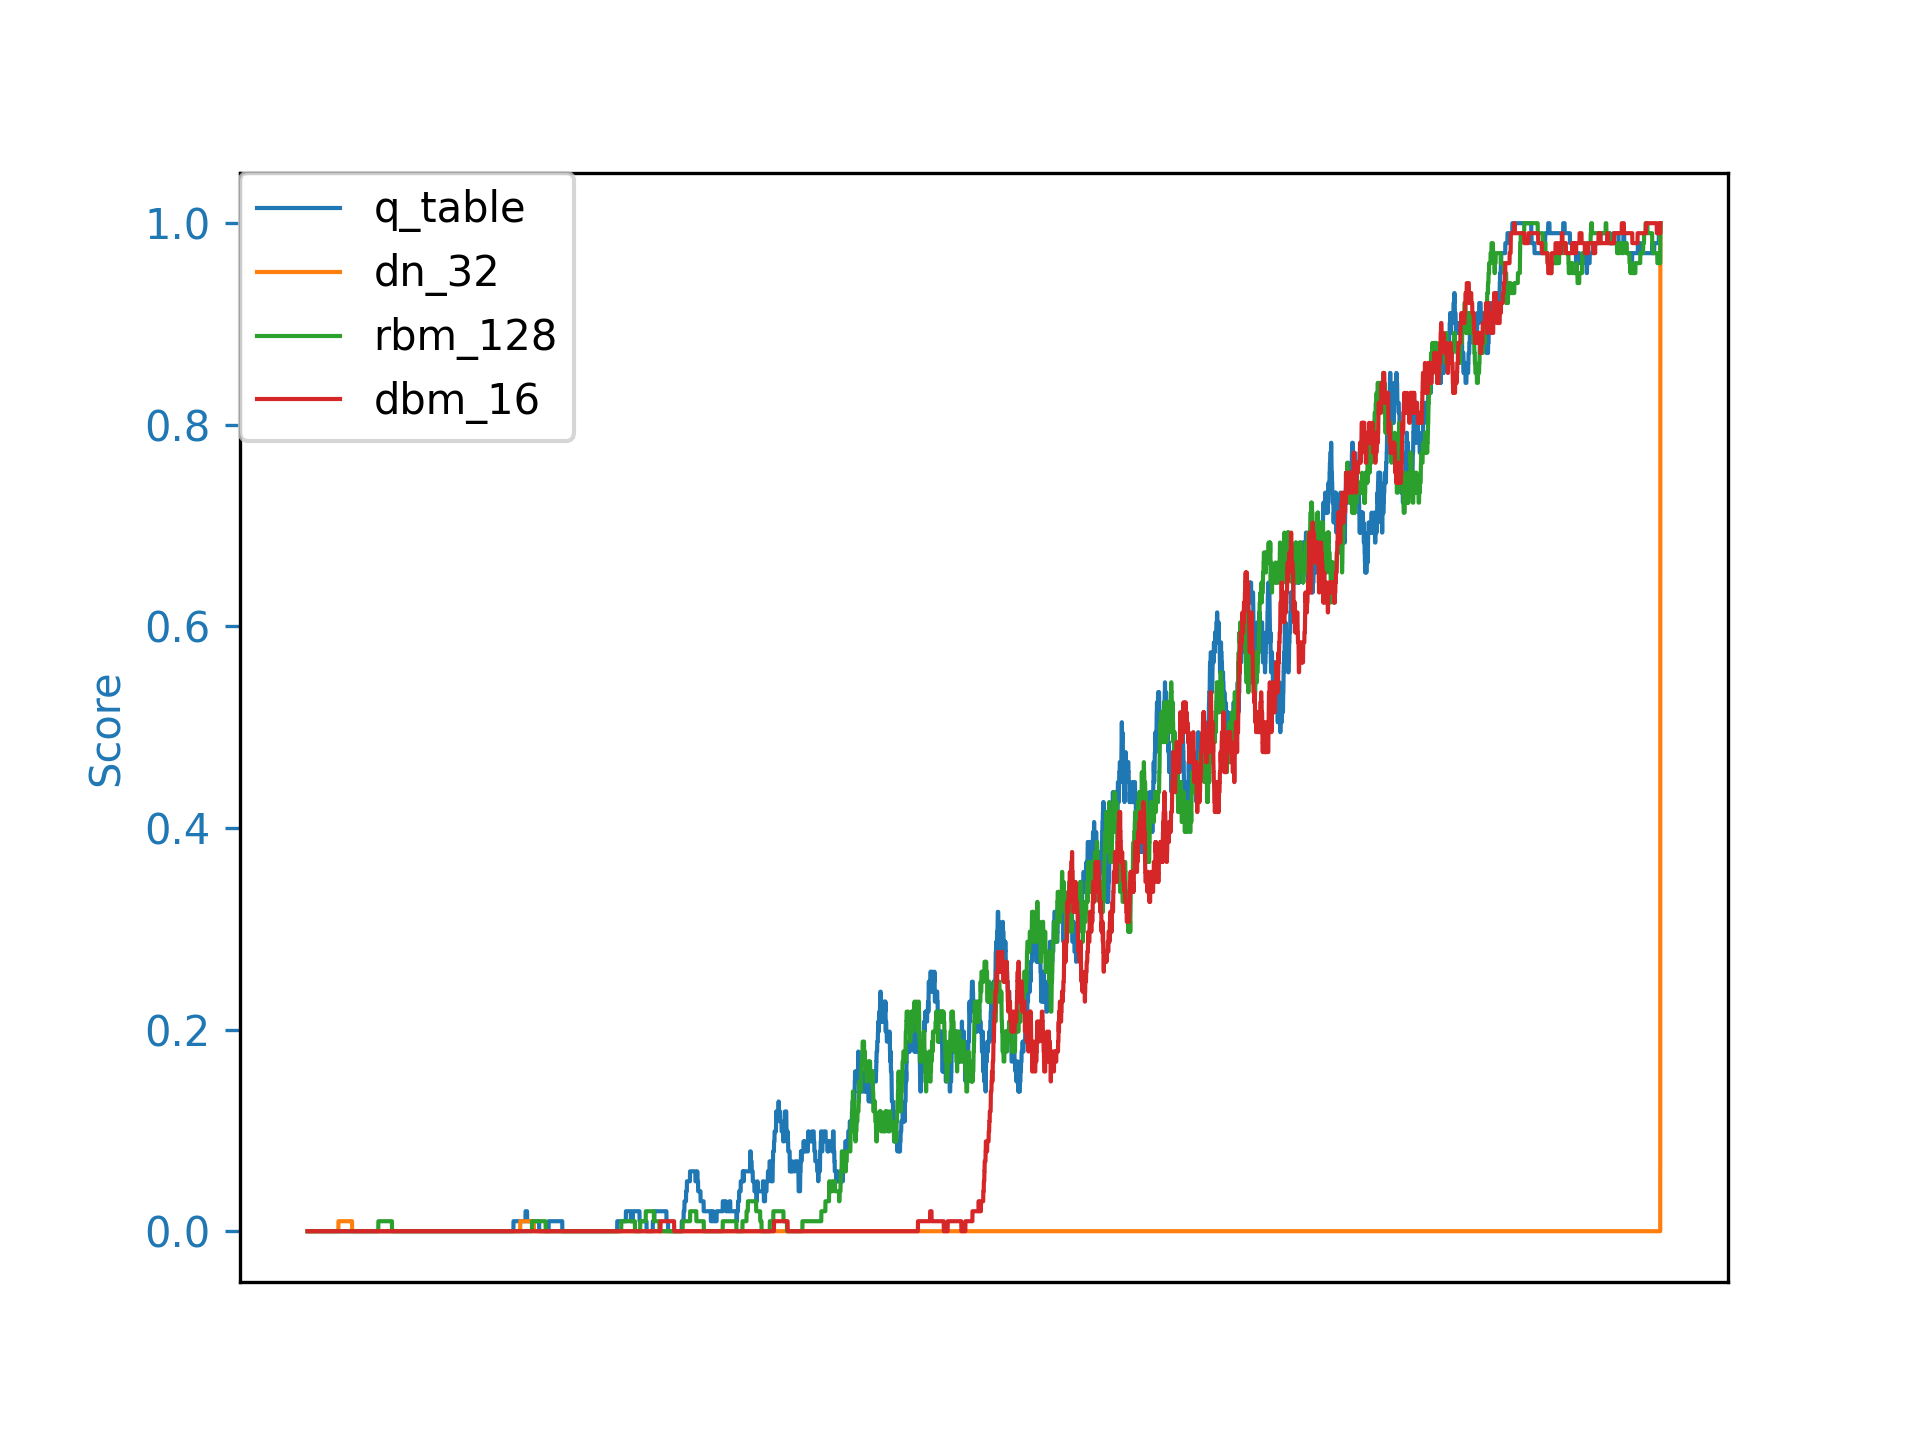
\includegraphics[width=\textwidth]{Figures/all_5x5_q_table_dn_32_rbm_128_dbm_16.png}
\caption{5x5 Alle Methoden}
\label{all_5}
\end{figure}

\begin{figure}[H]
\centering
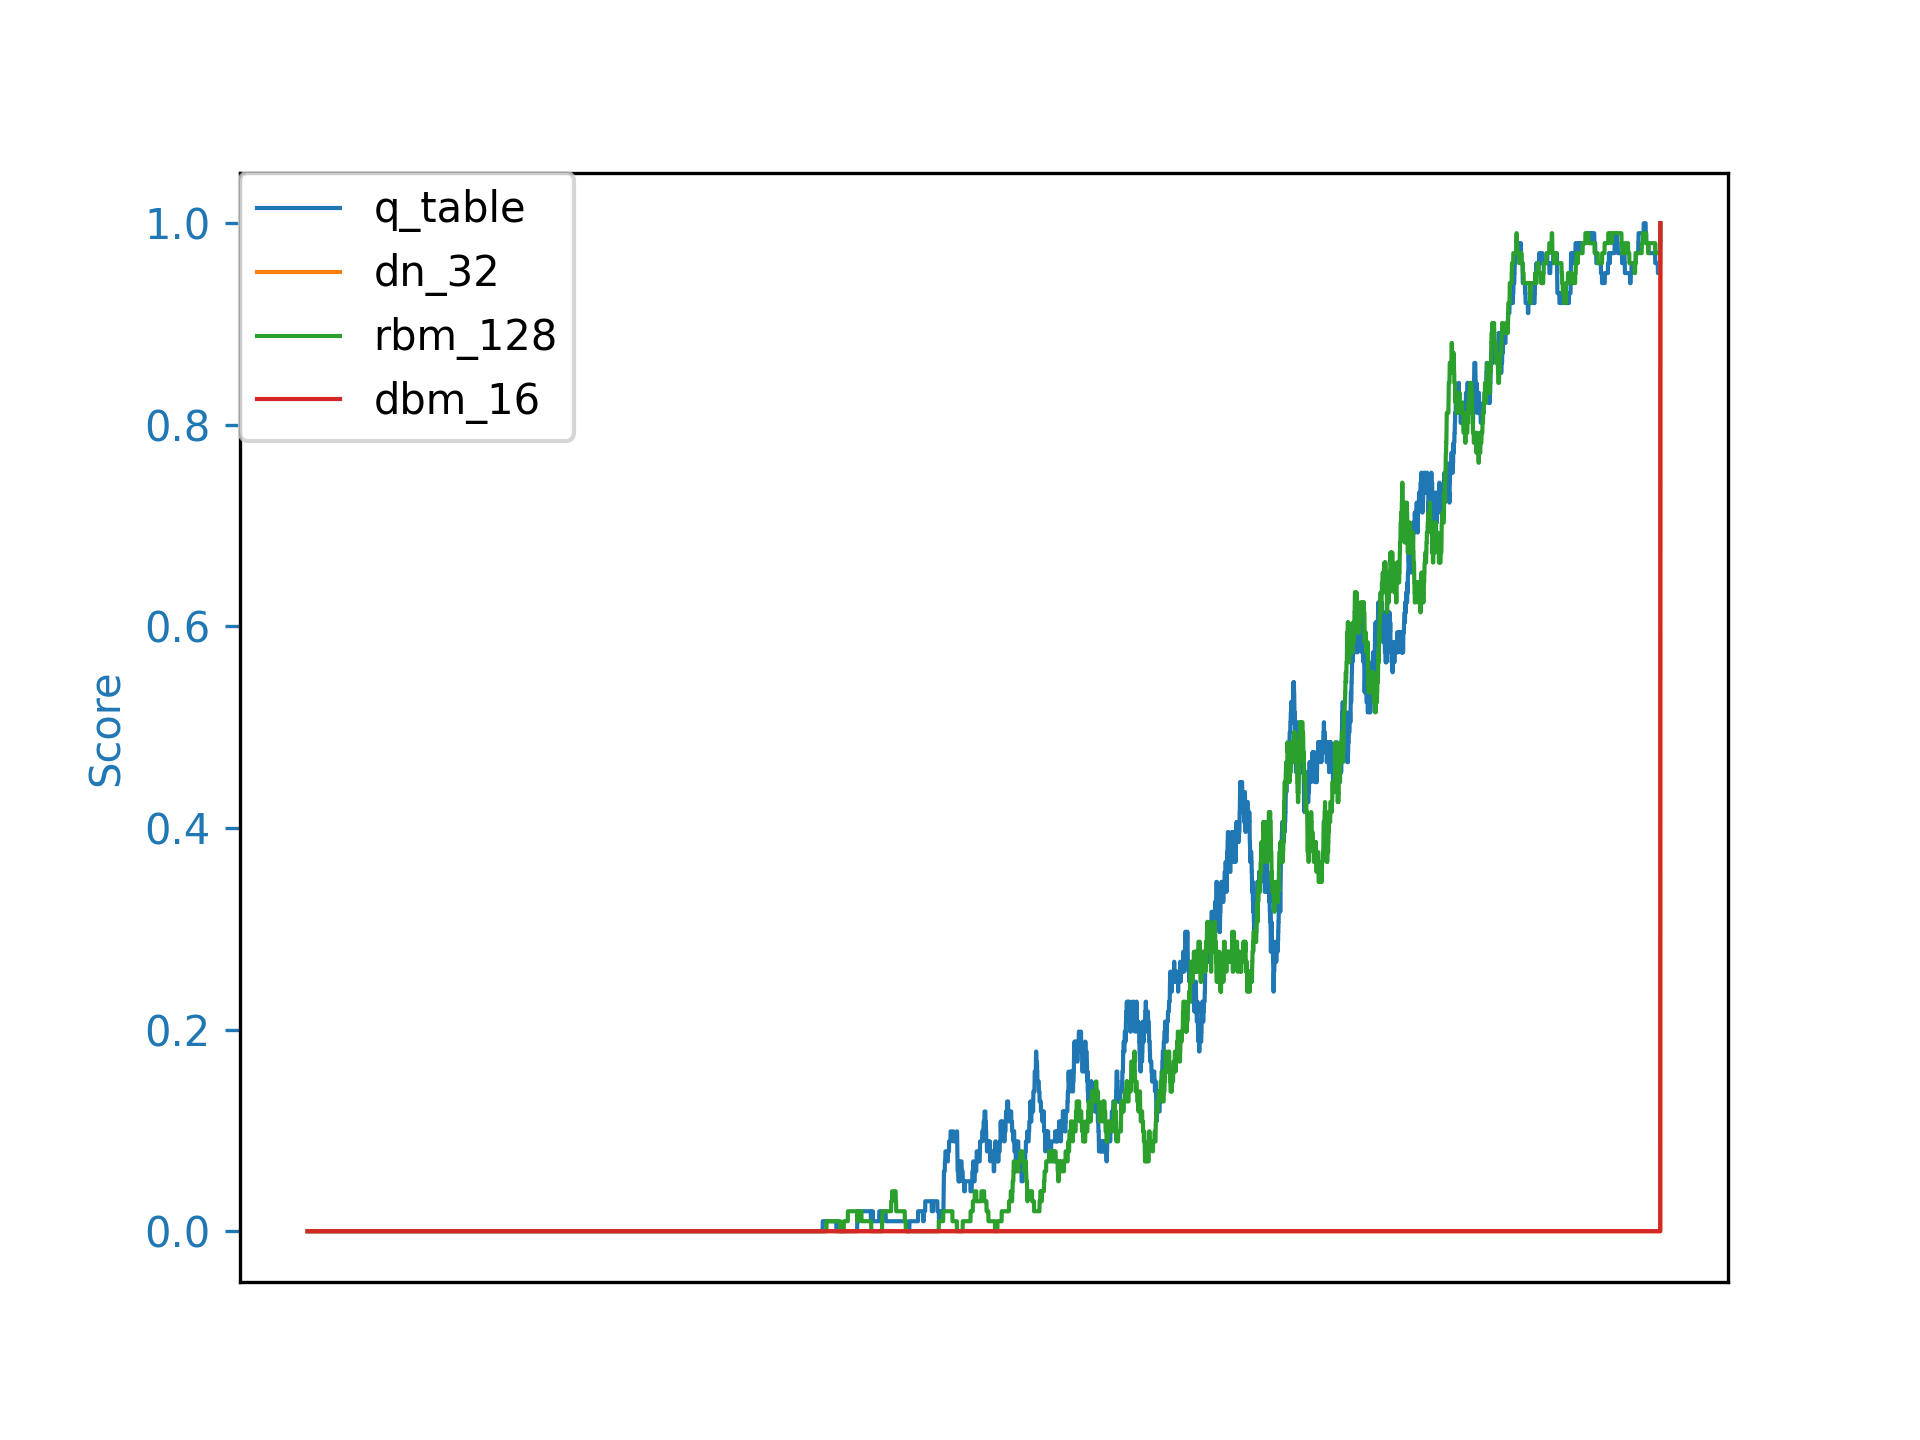
\includegraphics[width=\textwidth]{Figures/all_6x6_q_table_dn_32_rbm_128_dbm_16.png}
\caption{6x6 Alle Methoden}
\label{all_6}
\end{figure}

\begin{figure}[H]
\centering
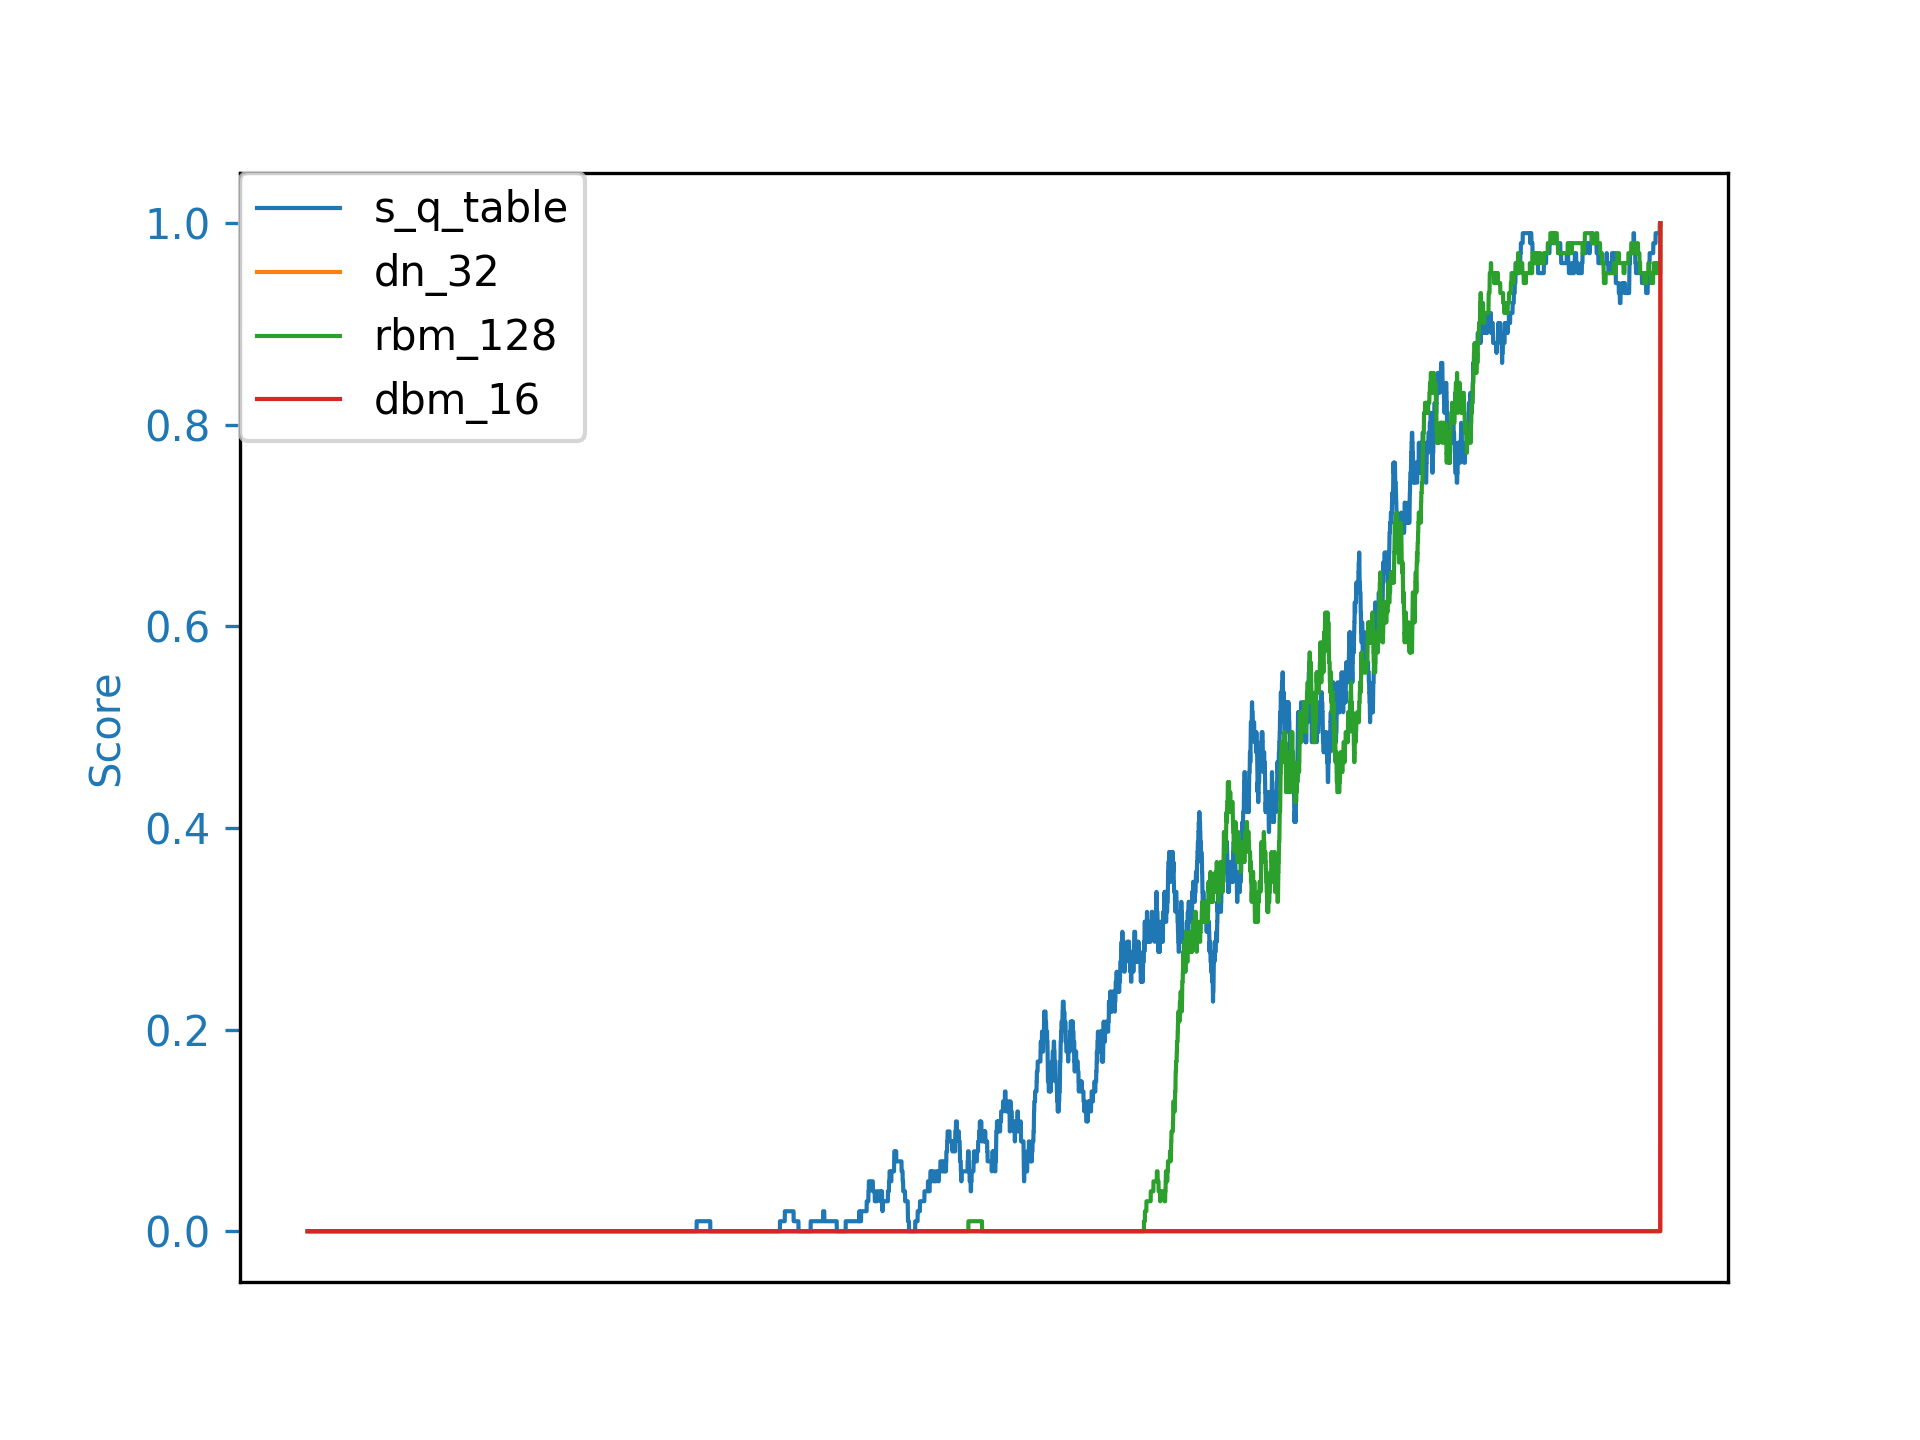
\includegraphics[width=\textwidth]{Figures/all_8x8_s_q_table_dn_32_rbm_128_dbm_16.png}
\caption{8x8 einfach Alle Methoden}
\label{all_7}
\end{figure}

\begin{figure}[H]
\centering
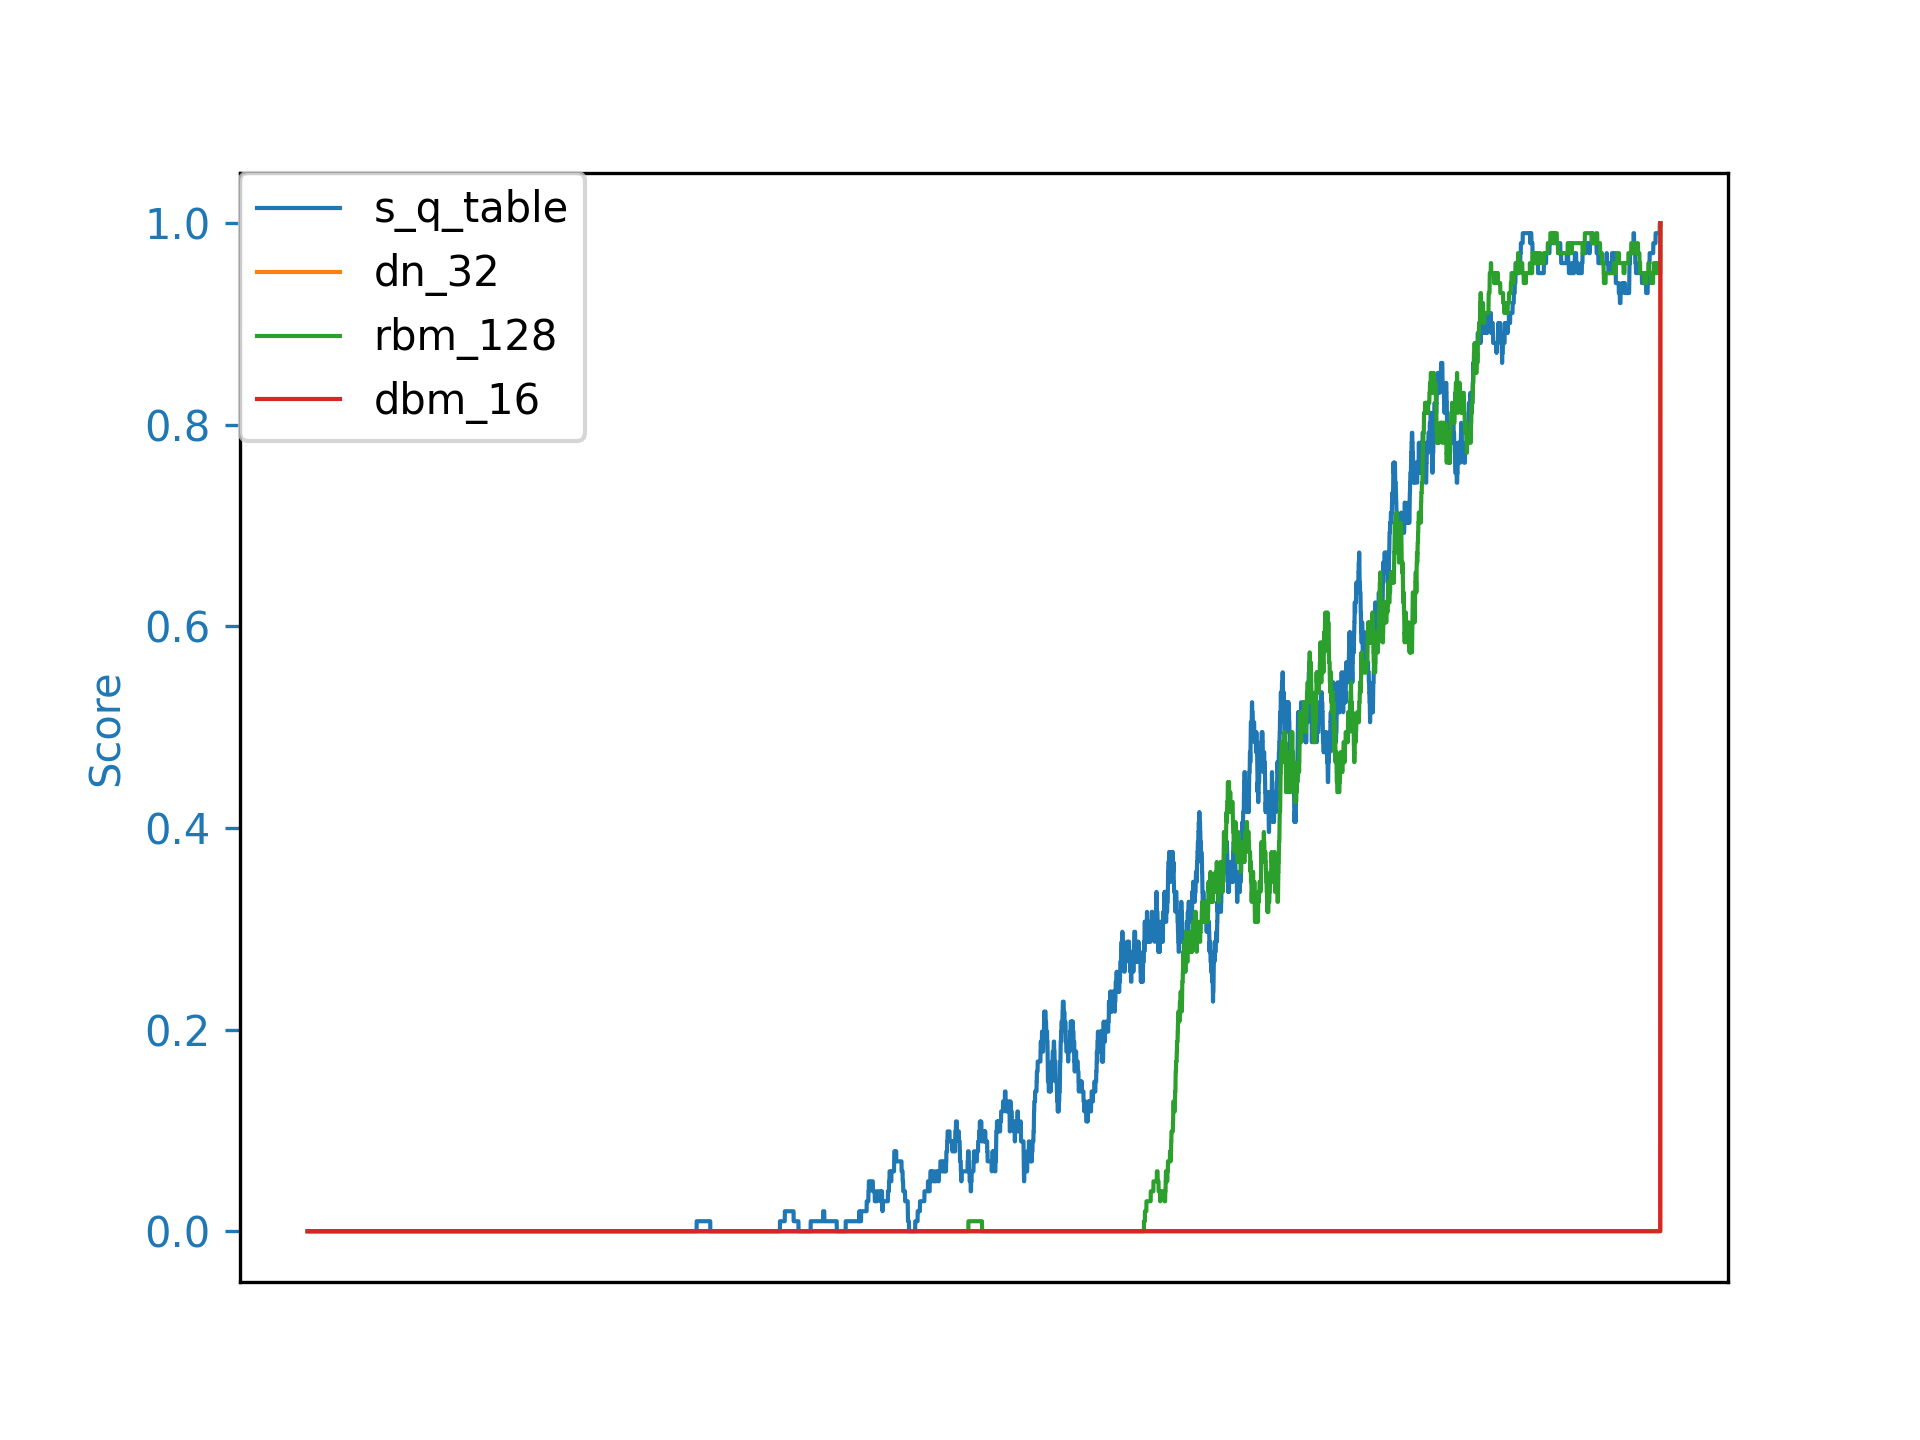
\includegraphics[width=\textwidth]{Figures/all_8x8_s_q_table_dn_32_rbm_128_dbm_16.png}
\caption{8x8 schwer Alle Methoden}
\label{all_8}
\end{figure}

\newpage

\begin{acknowledgement}
Wir bedanken uns bei allen Unterstützern!
\end{acknowledgement}